\RequirePackage[hyphens]{url}

\documentclass[12pt, a4paper, twoside, openright]{report}
%\documentclass[11pt, a4paper]{report}

\usepackage[utf8]{inputenc}
\usepackage[T1]{fontenc}
\usepackage{lmodern}
\usepackage{listings}
\usepackage{amsmath}
\allowdisplaybreaks
\usepackage{amsfonts}
\usepackage{amstext}
\usepackage{amssymb}
\usepackage{amsthm}
\usepackage{empheq}
\usepackage{cases}
\usepackage{anyfontsize}
\usepackage{enumitem}
\usepackage{pdfpages}
\usepackage{fourier}	% Style
\usepackage{bm}
\usepackage{epstopdf}
\usepackage{lipsum}
\usepackage{authblk}
%\usepackage[top=3cm, bottom=3cm, left=2cm, right=2cm, scale=0.75]{geometry}	% Set the margins
\usepackage[inner=3cm, textwidth=445pt, scale=0.75, top=3cm, bottom=3cm]{geometry}	% Set the margins
\usepackage{fancyhdr}
\usepackage[letterspace=150]{microtype}
\usepackage{textcomp}
\usepackage{gensymb}
\usepackage{booktabs}
\usepackage{amsmath,etoolbox}
\usepackage{mathtools}
\usepackage{anyfontsize}
%\usepackage{enumerate}
\usepackage{graphicx}
\usepackage{epstopdf}
\usepackage{float}
\usepackage{subfig}
\usepackage[labelfont=bf,labelsep=period,font=small]{caption}
\usepackage{newunicodechar}
\usepackage{nicefrac}	% For diagonal fractions
\usepackage{bbm}
\usepackage{csvsimple}
%\usepackage{floatrow}	% For notes below a figure

% Set header and footer
\usepackage{fancyhdr}
\pagestyle{fancy}
\fancyhf{}
\fancyhead[LE,RO]{\thepage}
\fancyhead[RE]{\nouppercase{\leftmark}}
\fancyhead[LO]{\nouppercase{\rightmark}}

% Packages needed for tables
\usepackage{longtable}
\usepackage{multicol}
\usepackage{multirow}
\usepackage{array}

\PassOptionsToPackage{hyphens}{url}\usepackage{hyperref}
\usepackage{breakurl}
\usepackage{url}

% To put footnotes at the bottom of the page
\usepackage[bottom]{footmisc}

% No indent
%\setlength\parindent{0pt}

% To enumerate subequations with arabic numbers (e.g. 1.1, 1.2, ecc)
%\patchcmd{\subequations}{\def\theequation{\theparentequation\alph{equation}}}{\def\theequation{\theparentequation.\arabic{equation}}}{}{}
\numberwithin{equation}{chapter}
%\usepackage{chngcntr}
%\counterwithout{equation}{section} % undo numbering system provided by phstyle.cls
%\counterwithin{equation}{chapter}  % implement desired numbering system

\DeclarePairedDelimiter\abs{\lvert}{\rvert}
\makeatletter
\let\oldabs\abs
\def\abs{\@ifstar{\oldabs}{\oldabs*}}

% Theorem and definition environment
\theoremstyle{theorem}
\newtheorem{theorem}{Theorem}[section]
\theoremstyle{definition}
\newtheorem{definition}{Definition}[chapter]
\theoremstyle{remark}
\newtheorem{remark}{Remark}[section]
\theoremstyle{proposition}
\newtheorem{proposition}{Proposition}[chapter]
%\newenvironment{definition}[1][Definition]{\begin{trivlist}
%\item[\hskip \labelsep {\bfseries #1}]}{\end{trivlist}}

% To enumerate the equations and the figures according to the section they are in
%\numberwithin{equation}{section}
\numberwithin{figure}{chapter}

% Path to images folder
\graphicspath{{./img/}}

% To modify the space between figure and caption
%\setlength{\abovecaptionskip}{-4pt}
%\setlength{\belowcaptionskip}{3pt}

\renewcommand{\textfraction}{0.1}
\renewcommand{\topfraction}{0.9}

\usepackage{empheq}

\usepackage{tikz}

% Python
% Default fixed font does not support bold face
\DeclareFixedFont{\ttb}{T1}{txtt}{bx}{n}{10.25} % for bold
\DeclareFixedFont{\ttm}{T1}{txtt}{m}{n}{10.25}  % for normal

% Custom colors
\usepackage{color}
\definecolor{deepblue}{rgb}{0,0,0.5}
\definecolor{deepred}{rgb}{0.6,0,0}
\definecolor{deepgreen}{rgb}{0,0.5,0}

\usepackage{listings}

% Python style for highlighting
\newcommand\pythonstyle{\lstset{
	language=Python,
	basicstyle=\ttm,
	otherkeywords={self},             % Add keywords here
	keywordstyle=\ttb\color{deepblue},
	emph={MyClass,__init__},          % Custom highlighting
	emphstyle=\ttb\color{deepred},    % Custom highlighting style
	stringstyle=\color{deepgreen},
	frame=tb,                         % Any extra options here
	showstringspaces=false            % 
}}


% Python environment
\lstnewenvironment{python}[1][]
{
	\pythonstyle
	\lstset{#1}
}
{}

% Python for external files
\newcommand\pythonexternal[2][]{{
		\pythonstyle
		\lstinputlisting[#1]{#2}}}

% Python for inline
\newcommand\pythoninline[1]{{\pythonstyle\lstinline!#1!}}

% C++ style for highlighting
\newcommand\cppstyle{\lstset{
	language=C++,
	basicstyle=\ttm,
	otherkeywords={},             % Add keywords here
	keywordstyle=\ttb\color{deepred},
	emph={int,double,bool,const,void,auto},          % Custom highlighting
	emphstyle=\ttb\color{deepgreen},    % Custom highlighting style
	stringstyle=\color{purple},
	commentstyle=\color{blue}\ttfamily,
	frame=tb,                         % Any extra options here
	showstringspaces=false            % 
}}

% C++ environment
\lstnewenvironment{cpp}[1][]
{
	\cppstyle
	\lstset{#1}
}
{}

% C++ for external files
\newcommand\cppexternal[2][]{{
		\cppstyle
		\lstinputlisting[#1]{#2}}}

% C++ for inline
\newcommand\cppinline[1]{{\cppstyle\lstinline!#1!}}

% Set listings options for R code
\lstset{
	language=R,
	basicstyle=\ttm,
	commentstyle=\ttfamily\color{blue},
	backgroundcolor=\color{white},
	frame=tb,
	showstringspaces=false,
	showtabs=false,
	tabsize=2,
	keywordstyle=\ttb\color{deepred},
	stringstyle=\color{purple},
	emph={NULL},          % Custom highlighting
	emphstyle=\ttb\color{purple},
}

% For argmin
\DeclareMathOperator*{\argmin}{arg\,min}

% To insert verbatim within a command
\usepackage{fancyvrb}

% For pseudocode
\usepackage[chapter]{algorithm}
\usepackage{algpseudocode}

\usepackage[many]{tcolorbox}

\makeatletter
	\renewcommand*\l@figure{\@dottedtocline{1}{1em}{3.2em}}
\makeatother

% Define norm symbol
\newcommand{\norm}[1]{\left\lVert#1\right\rVert}

% Define mod symbol
\newcommand{\Mod}[1]{\ (\mathrm{mod}\ #1)}

% Aliases for \boldsymbol and \widetilde
\newcommand{\wt}[1]{\widetilde{#1}}
\newcommand{\bg}[1]{\boldsymbol{#1}}

% Redefine \Require and \Ensure for algorithm environment
\renewcommand{\algorithmicrequire}{\textbf{Input:}}
\renewcommand{\algorithmicensure}{\textbf{Output:}}

% Make \big| adapt to the context
\makeatletter
\let\amstexbig\big
\def\newbig#1{%
  \ifx#1|%
    \expandafter\@firstoftwo
  \else
    \expandafter\@secondoftwo
  \fi
  {\big@bar}%
  {\amstexbig{#1}}%
}
\AtBeginDocument{\let\big\newbig}
\def\big@bar{\bBigg@{1.1}|}
\makeatother

% For blackboard-bold 0 and 1
%\usepackage[bb=boondox]{mathalfa}

\begin{document}

	\tableofcontents
	\listoffigures
	\listofalgorithms
	
	\chapter{Introduction to neural networks}
	\label{chapter:Introduction to neural networks}
	
		Let us start this dissertation by introducing the key components of an artificial neural network and discussing the way it can be configured for a specific application. Please note that this chapter is not meant to provide a comprehensive overview on neural networks, rather to investigate some aspects and concepts functional to the following chapters. For further reading, we refer the reader to, e.g., \cite{Hag14, Hay05, Kri}, from which we retrieved many of the informations provided in this chapter.
		
		Throughout this work we confine the attention to the most-spread neural network paradigm - the \emph{feedforward} neural network, presented in Section \ref{section:Network topologies} - employing the well-known \emph{backpropagation of error} as learning rule, derived in Section \ref{section:Training a multilayer feedforard neural network}. Actually, in the numerical experiments we carried out and whose results will be discussed in Chapter \ref{}, we mainly refer to a variant of backpropagation - the Levenberg-Marquardt algorithm.
		
		Before moving to the description of technical neural networks, let us provide a brief excursus on their biological counterparts. The goal is to highlight the basic features of the human nervous system, focusing on the working principles of neurons and the way informations are processed, thus to extract the key concepts which should be taken over into a mathematical, simplified representation.
		
	\vspace*{0.3cm} 
		
	\section{Biological motivation}
	\label{section:Biological motivation} 
	
		\begin{figure}[t]
			\center
			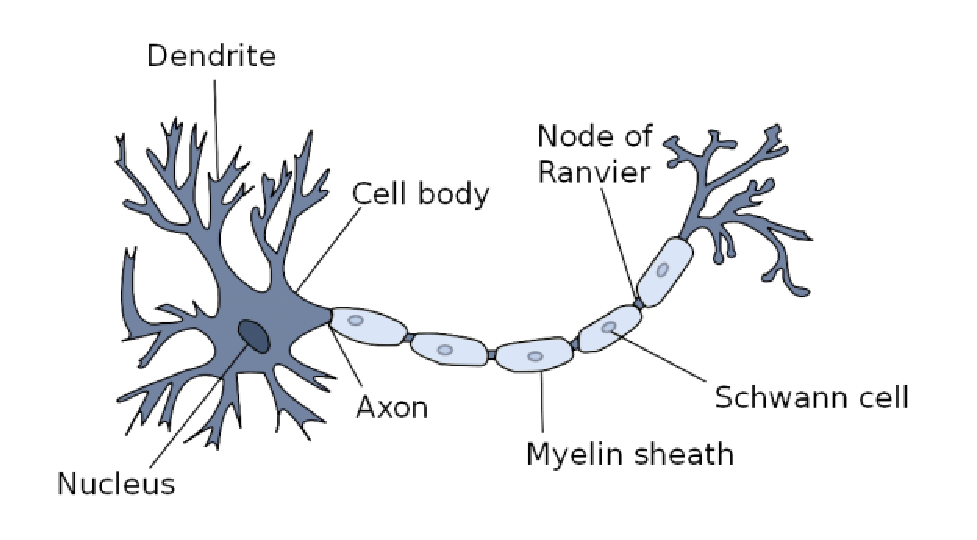
\includegraphics[scale = 0.5]{neuron.eps}
			
			\caption{Simplified representation of a biological neuron, with the components discussed in the text; retrieved from \cite{Kri}.}
			\label{fig:neuron}
		\end{figure}
		
		The information processing system of a vertebrate can coarsely be divided into the \emph{central nervous system} (CNS) and the \emph{peripheral nervous system} (PNS). The former consists of the \emph{brain} and the \emph{spinal cord}, while the latter mainly comprises the \emph{nerves}, which transmit informations from all other parts of the body to the CNS (\emph{sensory nerves}) and viceversa (\emph{motor nerves}). When an output stimulus hits the sensory cells of an organ sense, these generate an electric signal, called \emph{sensory signal}, which is transfered to the central nervous system via the \emph{sensory nerves}. Within the CNS, informations are stored and managed to provide the muscles with a suitable \emph{motor signal}, broadcast through the \emph{motor nerves} and finally converted by the effectors into a system output \cite{Hay05}. %In addition, the central nervous system is also in charge of controlling the inner processes in the body and coordinating motor functions \cite{Kri}.
		
		Hence, both the central and peripheral nervous system are directly involved in the information processing workflow. At the cellular level, this is accomplished through a huge amount of modified cells called \emph{neurons}. These processing elements continuosly communicate each other by means of electric signals, traveling through a thick net of connections. For instance, in a human being each neuron is linked in average with $10^3 - 10^4$ other neurons. As detailed in the next paragraph, a neuron is characterized by a rather simple structure, specifically designed to rapidly collect input signals and generate an output pulse whenever the accumulated incoming signal exceeds a threshold - the \emph{action potential}. In other terms, a neuron acts as a switch, establishing a typically nonlinear input-output mapping \cite{Kri}.
		
		From a simplifying perspective, a neuron consists of three main components: the \emph{dendrites}, the \emph{nucleus} or \emph{soma}, and the \emph{axon}. Dendrites are tree-like networks of nerve fibers receiving input signals from many sources and conveying them directly to the nucleus of the neuron. Here, input signals are accumulated and thresholded, as mentioned before. The possible output pulse is then broadcast to the cells contiguous the neuron through the axon - a unique, slender fiber constituing an extension of the soma and splitting in many branches at the opposite extremity \cite{SD13}. To ease the electrical conduction of the signal, the axon is isolated through a myelin sheath which consists of Schwann cells (in the PNS) or oligodendrocytes (in the CNS). However, this insulating film is not continuous, rather presents gaps at regular intervals called \emph{nodes of Ranvier}, which lets the signal be conducted in a saltatory way.
		
		The signal coming from the axon of another neuron or from another cell is transfered to the dendrites of a neuron through a particular connection called \emph{synapsis}\footnote{For the sake of completeness, we mention that there exist synapses directly connecting the axon of the sender neuron with either the soma or the axon of the receiver. Actually, a synapsis may also connect the axon of a neuron with the dendrite or soma of the same neuron (autosynapsis). However, for our purposes we can confine the attention to the axon-dendrite synapsis.}. A synaptic may be either electrical or chemical. In the former, the presynaptic side, i.e., the sender axon, and the postsynapic side, i.e., the receiver dendrite, are directly in contact, so that the potential can simply travel by electrical conduction. Conversely, a chemical synapsis consists of a synaptic \emph{cleft}, physically separating the presynaptic side from the postsynaptic side. Then, to let the action potential reach the postsynaptic side, at the presynaptic side the electrical pulse is converted into a chemical signal. This is accomplished by releasing some chemical substances called \emph{neurotransmitters}. These neurotransmitters then cross the cleft and bind to the receptors dislocated onto the membrane of the postsynaptic side, where the chemical signal is re-converted into an electrical potential. On the other hand, neurotransmitters do not simply broadcast the action potential. Indeed, we can distinguish between excitatory and inhibitory neurotransmitters, respectively amplifying or modulating the signal. Hence, the pulse outgoing a neuron is preprocessed within the synapsis before reaching the target cell. In other terms, a neuron gets in input many \emph{weighted} signals, which should then be collected.
		
		 Different studies have unveiled the tight correlation between the synapses the neurons establish among each other, and the tasks a neural network can address \cite{Hag14}. That is, the set of interneuron connection strengths represent the information storage, i.e., the knowledge, of a neural network \cite{Kri}. Knowledge is acquired through a \emph{learning} or \emph{training} process, entailing adjustments at the synaptic level to adapt to environmental situations. The adjustments may not only involve the modification of existing synapses, but also the creation of new synaptic connections. Hence, the nervous system is a distributed memory machine whose evolutionary structure is shaped by experience.
		 
		 As mentioned above, a biological neural network acquaints itself with problems of a specific class through a learning procedure. During the learning, the network is exposed to a collection of situations, giving it the possiblity to derive a set of tools which will let it provide reasonable solutions in similar circumstances. In other terms, the cognitive system should be able to \emph{generalize}. Furthermore, after a successfull training a neural network should also show a discrete level of \emph{fault tolerance} against external errors, e.g. noisy inputs. It worths notice here that the nervous system is also naturally fault tolerant against \emph{internal} errors. Indeed, in case a neuron or a (relatively small) group of neurons got damaged or died, the other processing nodes would take care of its tasks, so that the overall cognitive capabilities would be only slightly affected \cite{Kri}. 
		 
		 %Lastly, let us point out that, since neurons operate in synergy and knowledge is shared among synapses, a biological neural network provides an example of a large-scale \emph{parallel}, {distributed memory} system. Furthermore, in case a neuron or a (relatively small) group of neurons got damaged or died, the other processing nodes would take care of its tasks, so that the overall cognitive capabilities would be only slightly affected \cite{Kri}. In other terms, a neural network shows an high level of \emph{fault tolerance} against internal errors.
		 
	\vspace*{0.3cm}
		 		
	\section{Artificial neural networks}
	\label{section:Artificial neural networks}
				
		Inspired by the biological information processing system discussed so far, an artificial neural network (ANN), usually simply referred to as "neural network", is a computational model capable to learn from observational data, i.e., by example, thus providing an alternative to the algorithmic programming paradigm \cite{Nie15}. Exactly as its original counterpart, it consists of a collection of processing units, called (artificial) neurons, and directed weighted synaptic connections between the neurons themselves. Data travel among neurons through the connections, following the direction imposed by the synapses themselves. Hence, an artificial neural network is an \emph{oriented graph} to all intents and purposes, with the neurons as \emph{nodes} and the synapses as oriented \emph{edges}, whose weights are adjusted by means of a \emph{training} process to configure the network for a specific application \cite{SD13}. 
		
		Formally, a neural network could be defined as follows \cite{Kri}.
		
		\begin{definition}[Neural network]
			\label{def:neural-network}
			\emph{
			A \emph{neural network} is a sorted triple $\left( \mathcal{N} \, , \mathcal{V} \, , w \right)$, where $\mathcal{N}$ is the set of \emph{neurons}, with cardinality $|\mathcal{N}|$, $\mathcal{V} = \big\lbrace (i \, , j), \, 1 \leq i \, , j  \leq |\mathcal{N}| \big\rbrace$ is the set of \emph{connections}, with $(i,j)$ denoting the oriented connection linking the sending neuron $i$ with the target neuron $j$, and $w : \mathcal{V} \rightarrow \mathbb{R}$ is the \emph{weight function}, defining the weight $w_{i,j} = w((i,j))$ of the connection $(i,j)$. A weight may be either positive or negative, making the underlying connection either excitatory or inhibitory, respectively. By convention, $w_{i,j} = 0$ means that neurons $i$ and $j$ are not directly connected.
			}
		\end{definition}
		
		In the following, we dive deeper into the structure and training of a neural network, starting by detailing the structure of an artificial neuron.  
		
	\vspace*{0.3cm}
														
	\subsection{Neuronal model}
	\label{section:Neuronal model}
	
		As its name may suggest, an artificial neuron represents a simplified model of a biological neuron, retaining its main features discussed in Section \ref{section:Biological motivation}. To introduce the components of the model, let us consider the neuron $j$ represented in Figure \ref{fig:neural-model}. Suppose that it is connected with $m$ sending neurons $s_1, \, \ldots \, , s_m$, and $n$ receiving (target) neurons $r_1, \, \ldots \, , r_n$. Denoting by $y_{\Omega}(t) \in \mathbb{R}$ the scalar output fired by a generic neuron $\Omega$ at time $t$, neuron $j$ gets the weighted inputs $w_{s_k,j} ~ y_{s_k}(t)$, $k = 1, \, \ldots \, , m$, at time $t$, and sends out the output $y_j(t + \Delta t)$ to the target neurons $r_1, \, \ldots \, , r_n$ at time $t + \Delta t$. Please note that in the context of artificial neural networks the time is discretized by introducing the timestep $\Delta t$. This is clearly not plausible from a biological viewpoint; on the other hand, it dramatically eases the implementation. In the following, we will avoid to specify the dependence on time unless strictly necessary, thus to lighten the notation.
		
		An artificial neuron $j$ is completely characterized by three functions: the propagation function, the activation function, and the output function. These will be defined and detailed hereunder in the same order they get involved in the data flow. 
		
		\vspace*{0.3cm}
		
		\noindent \textbf{Propagation function}. The propagation function $f_{prop}$ converts the vectorial input $\boldsymbol{p} = [y_{s_1}, \, \ldots \, , y_{s_m}]^T \in \mathbb{R}^m$ into a scalar $u_{j}$ often called \emph{net input}, i.e.,
		\begin{equation}
			\label{eq:propagation-function}
			u_{j} = f_{prop}(w_{s_1,j}, \, \ldots \, , w_{s_m,j}, \, y_{s_1}, \, \ldots \, , y_{s_m}) \, .
		\end{equation}
		A common choice for $f_{prop}$ (used also in this work) is the weighted sum, adding up the scalar inputs multiplied by their respective weights:
		\begin{equation}
			\label{eq:weighted-sum}
			f_{prop}(w_{s_1,j}, \, \ldots \, , w_{s_m,j}, \, y_{s_1}, \, \ldots \, , y_{s_m}) = \sum_{k = 1}^m w_{s_k,j} ~ y_{s_k} \, .
		\end{equation} 
		The function \eqref{eq:weighted-sum} provides a simple yet effective way of modeling the accumulation of different input electric signals within a biological neuron; this motivates its popularity.
		
		\begin{figure}[t]
			\center
			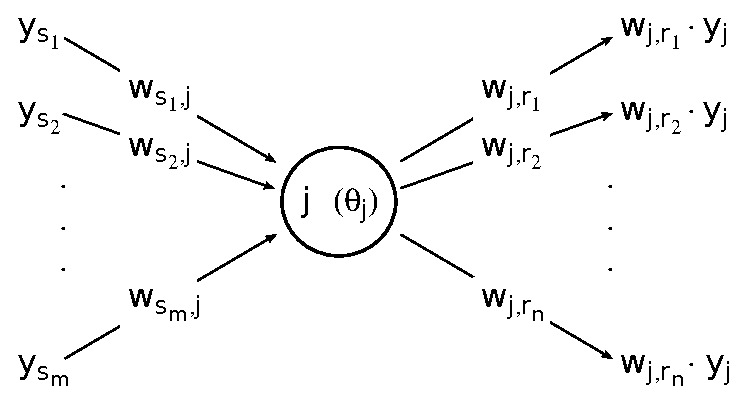
\includegraphics[scale = 0.6]{neural_model_ter.eps}
			
			\caption{Visualization of the generic $j$-th neuron of an artificial neural network. The neuron accumulates the weighted inputs $\big\lbrace w_{s_1,j} ~ y_{s_1}, \, \ldots \, , w_{s_m,j} ~ y_{s_m} \big\rbrace$ coming from the sending neurons $s_1, \, \ldots \, , s_m$, and fires $y_j$, sent to the target neurons $\big\lbrace r_1, \, \ldots \, , r_n \big\rbrace$ through the synapsis $\big\lbrace w_{j,r_1}, \, \ldots \, , w_{j,r_n} \big\rbrace$. The neuron threshold $\theta_j$ is reported within its body.} 
			\label{fig:neural-model}
		\end{figure}
		
		\vspace*{0.3cm}
		
		\noindent \textbf{Activation or transfer function}. At each timestep, the \emph{activation state} $a_j$, often shortly referred to as \emph{activation}, quantifies at which extent neuron $j$ is currently active or excited. It results from the activation function $f_{act}$, which combines the net input $u_j$ with a threshold $\theta_j \in \mathbb{R}$ \cite{Kri}: 
		\begin{equation}
			\label{eq:activation-function}
			a_j = f_{act}(u_j; \theta_j) = f_{act}(\sum_{k = 1}^m w_{s_k,j} ~ y_{s_k} \, ; \theta_j) \, ,
		\end{equation}
		where we have employed the weighted sum \eqref{eq:weighted-sum} as propagation function. From a biological perspective, the threshold $\theta_j$ is the analogous of the action potential mentioned in Section \ref{section:Biological motivation}. Mathematically, it represents the point where the absolute value $|f'_{act}|$ of the derivative of the activation function is maximum. Then, the activation function reacts particularly sensitive when the net input $u_j$ hits the threshold value $\theta_j$ \cite{Kri}. \\
		Furthermore, noting that $\theta_j$ is a parameter of the network, one may like to adapt it through a training process, exactly as can be done for the synaptic weights, as we shall see in Section \ref{section:Training a multilayer feedforard neural network}. However, $\theta_j$ is currently incorporated in the activation function, making its runtime access somehow cumbersome. This is typically overcome by introducing a \emph{bias neuron} in the network. A bias neuron is a continuously firing neuron, with constant output $y_{b} = 1$, which gets directly connected with neuron $j$, assigning the \emph{bias weight} $w_{b,j} = - \theta_j$ to the connection. As can be deduced by Figure \ref{fig:neural-model-bias}, $\theta_j$ is now treated as a synaptic weight, while the neuron threshold is set to zero. Moreover, the net input becomes
		\begin{equation}
			\label{eq:net-input}
			u_j = \sum_{k = 1}^m w_{s_k,j} ~ y_{s_k} - \theta_j \, ,
		\end{equation}
		i.e., the threshold is now included in the propagation function rather than in the activation function, which we can now express in the form
		\begin{equation}
			a_j = f_{act}(\sum_{k = 1}^m w_{s_k,j} ~ y_{s_k} - \theta_j) \, .
		\end{equation}
		Let us point out that this trick can be clearly applied to all neurons in the network which are characterized by a non-vanishing threshold: just connect the neuron with the bias, weighting the connection by the opposite of the threshold value. However, for ease of illustration in the following we shall avoid to include the bias neuron in any graphical representation of a neural network.
		
		Conversely to the propagation function, there exist various choices for the activation function, as the Heaviside or binary function, which assumes only $0$ or $1$, according to whether the argument is negative or positive, respectively:
		\begin{equation}
			\label{eq:heaviside}
			f_{act}(v) = 
			\begin{cases}
				& 0 \, , \hspace*{0.3cm} \text{if $v < 0$,} \\
				& 1 \, , \hspace*{0.3cm} \text{if $v \geq 0$.}
			\end{cases}
		\end{equation}
		Neurons characterized by such an activation function are usually named McCulloch-Pitts neurons, after the seminal work of McCulloch and Pitts \cite{Hay05}, and their employment is usually limited to single-layer perceptrons implementing boolean logic (see Section \ref{section:Network topologies}). In addition, note that \eqref{eq:heaviside} is discontinuous, with a vanishing derivative everywhere except that in the origin, thus not admissible for the backpropagation training algorithm presented in Section \ref{section:Training a multilayer feedforard neural network}. \\
		Among continuous activation maps, sigmoid functions have been widely used for the realization of artificial neural networks due to their graceful combination of linear and nonlinear behaviour \cite{Hay05}. Sigmoid functions are s-shaped and monotically increasing, and assume values in a bounded interval, typically $[0,1]$, as the logistic function,
		\begin{equation}
			\label{eq:logistic}
			f_{act}(v) = \dfrac{1}{1 + e^{\nicefrac{-v}{T}}} \hspace*{0.3cm} \text{with $T > 0$} \, ,
		\end{equation}
		or $[-1,1]$, as the hyperbolic tangent,
		\begin{equation}
			\label{eq:hyperbolic-tangent}
			f_{act}(v) = \dfrac{e^{v} - e^{-v}}{e^v + e^{-v}} \, .
		\end{equation}
		Both functions are displayed in Figure \ref{fig:activation-functions}. Note that the logistic function resemble the Heaviside function as $T$ decreases.
		
		\vspace*{0.3cm}
		
		\noindent \textbf{Output function}. Finally, the output function $f_{out}$ is in charge of calculating the scalar \emph{output} $y_j \in \mathbb{R}$ based on the activation state $a_j$ of the neuron:
		\begin{equation}
			\label{eq:output-function}
			y_j = f_{out}(a_j) \, ;
		\end{equation} 
		typically, $f_{out}$ is the identity function, so that activation and output of a neuron coincides, i.e., $y_j = f_{out}(a_j) = a_j$. Let us point out that while the input $\boldsymbol{p} = [y_{s_1}, \, \ldots \, , y_{s_m}]^T \in \mathbb{R}^m$ of the neuron is generally vectorial, i.e., $m > 1$, the output is scalar. The output $y_j$ could then either be sent to other neurons, included the outputting neuron itself (autosynapsis), or constitute a component of the overall output vector of the network, as for the neurons in the output layer of a feedforward neural network (see Section \ref{section:Network topologies}). \\
		It worths mention here that, as the activation function, also the output function is usually \emph{globally} defined, i.e., all neurons in the network (or at least a group of neurons) are equipped with the same output function.
		
		\begin{figure}[t]
			\center
			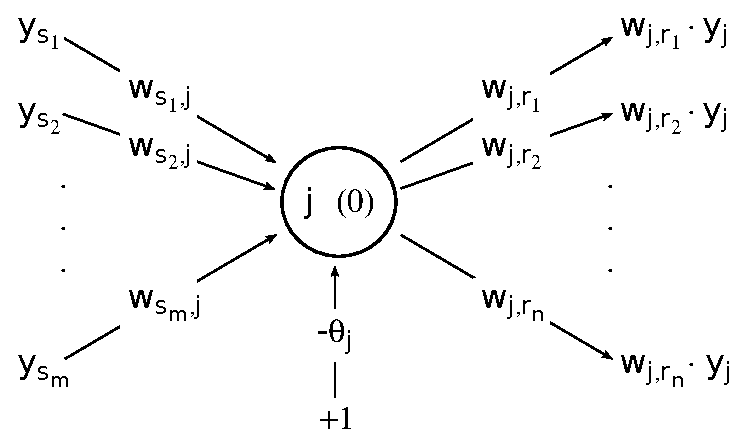
\includegraphics[scale = 0.6]{neural_model_bias.eps}
			
			\caption{Visualization of the generic $j$-th neuron of an artificial neural network. The neuron accumulates the weighted inputs $\big\lbrace w_{s_1,j} ~ y_{s_1}, \, \ldots \, , w_{s_m,j} ~ y_{s_m}, \, -\theta_j \big\rbrace$ coming from the sending neurons $s_1, \, \ldots \, , s_m, \, b$, respectively, with $b$ the bias neuron. The neuron output $y_j$ is then conveyed towards the target neurons $\big\lbrace r_1, \, \ldots \, , r_n \big\rbrace$ through the synapsis $\big\lbrace w_{j,r_1}, \, \ldots \, , w_{j,r_n} \big\rbrace$. Observe that, conversely to the model offered in Figure \ref{fig:neural-model}, the neuron threshold is now set to $0$.} 
			\label{fig:neural-model-bias}
		\end{figure}
		
		\vspace*{0.3cm}
		
		The neural model presented so far actually refers to the so called \emph{computing} neuron, i.e., a neuron processing input informations to provide a response. However, in a neural network one may also distinguish \emph{source} neurons, supplying the network with the respective components of the activation pattern (input vector) \cite{Hay05}. The role of source neurons will be clearer in the next section, where we will introduce the multilayer feedforward neural network. Here we just mention that such a neuron receives a scalar and unweighted input, which is simply forward to the connected neurons; no computations are performed.
		
	\vspace*{0.3cm}
		
	\subsection{Network topologies: the feedforward neural network}
	\label{section:Network topologies}
			
		The way neurons are interconnected within a network defines the \emph{topology} of the network itself, i.e., its design. In literature, many network architectures have been proposed, sometimes tailored to a specific application or task. In this section, we expand our investigation for the two most common network topologies: the feedforward and the recurrent neural network.
		
		\begin{figure}[t]
			\center
			\hspace*{-0.4cm}
			\subfloat{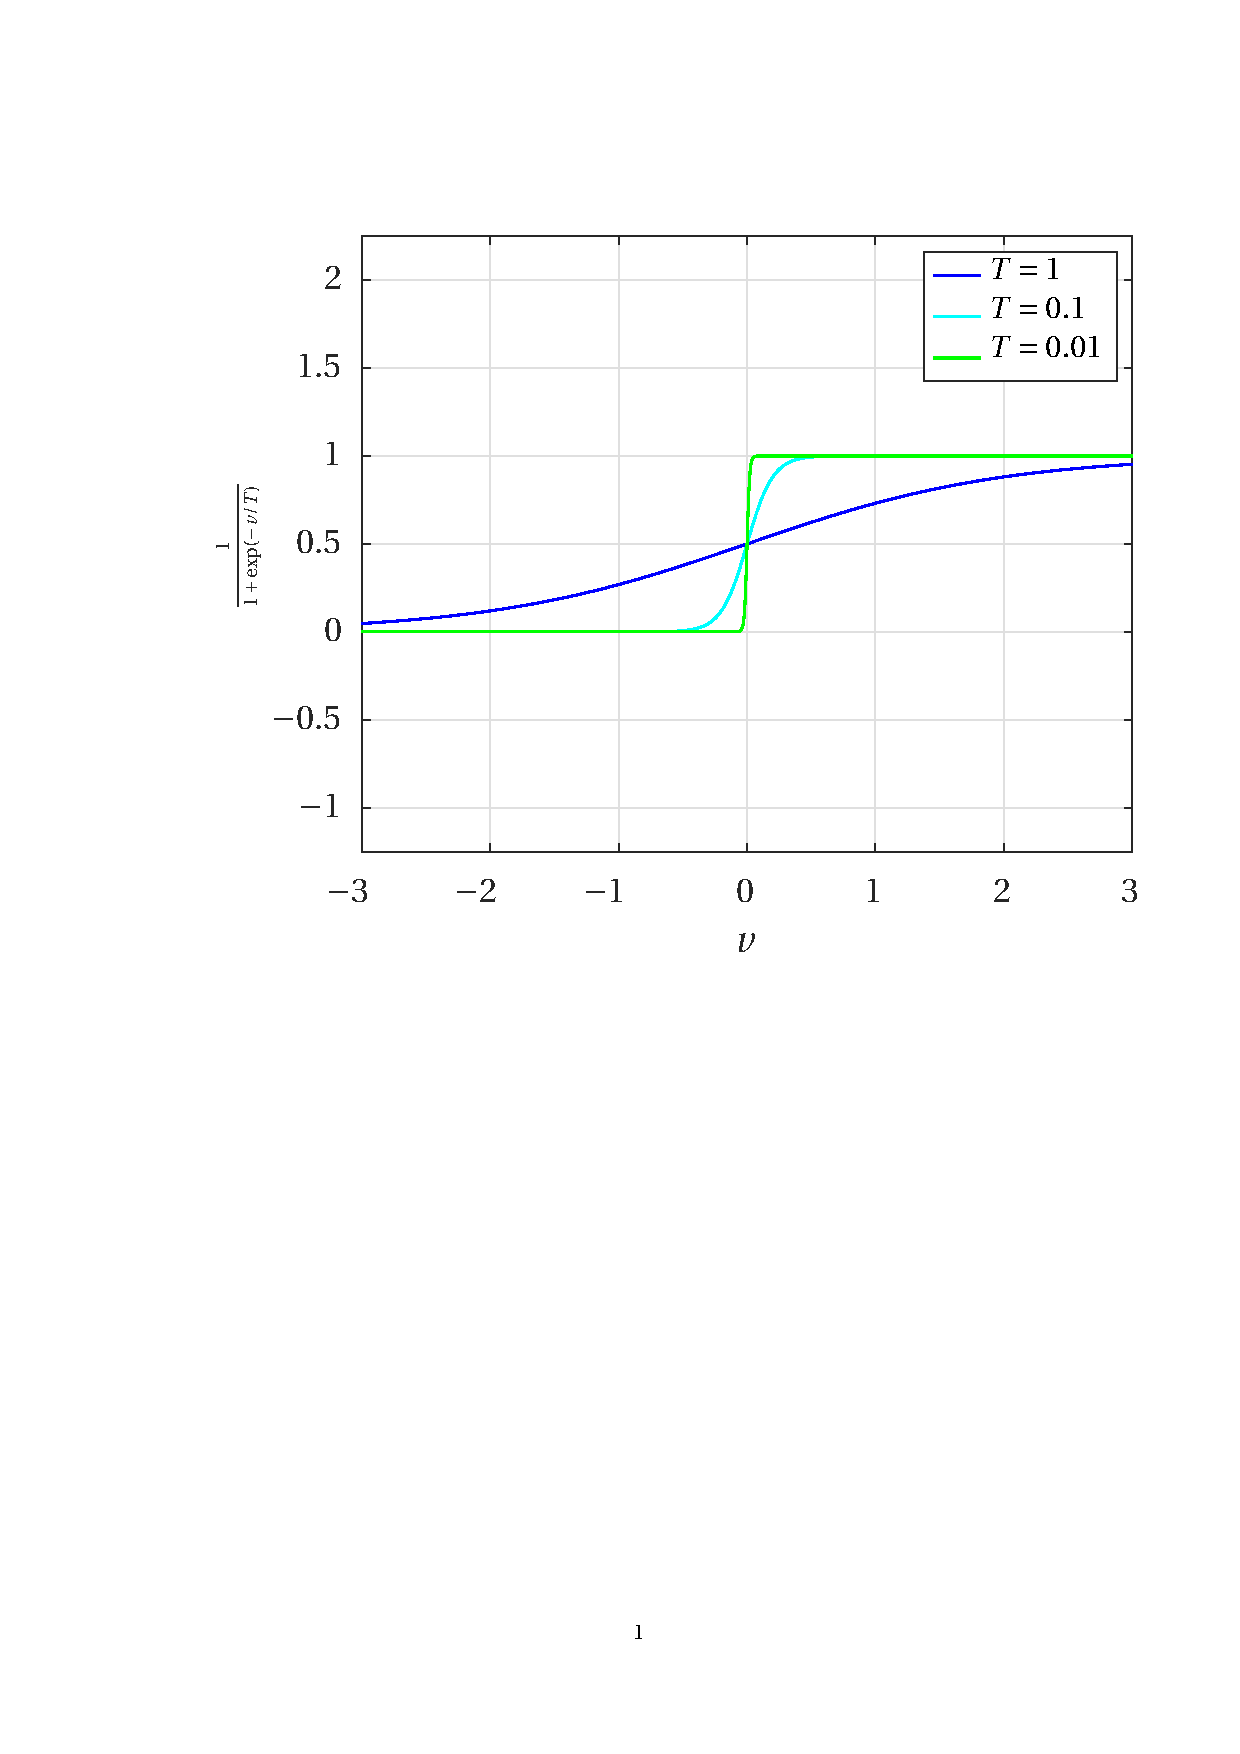
\includegraphics[scale = 0.44, trim = {2.5cm 13cm 1cm 3.5cm}, clip]{fermi_function_bis}}
			\subfloat{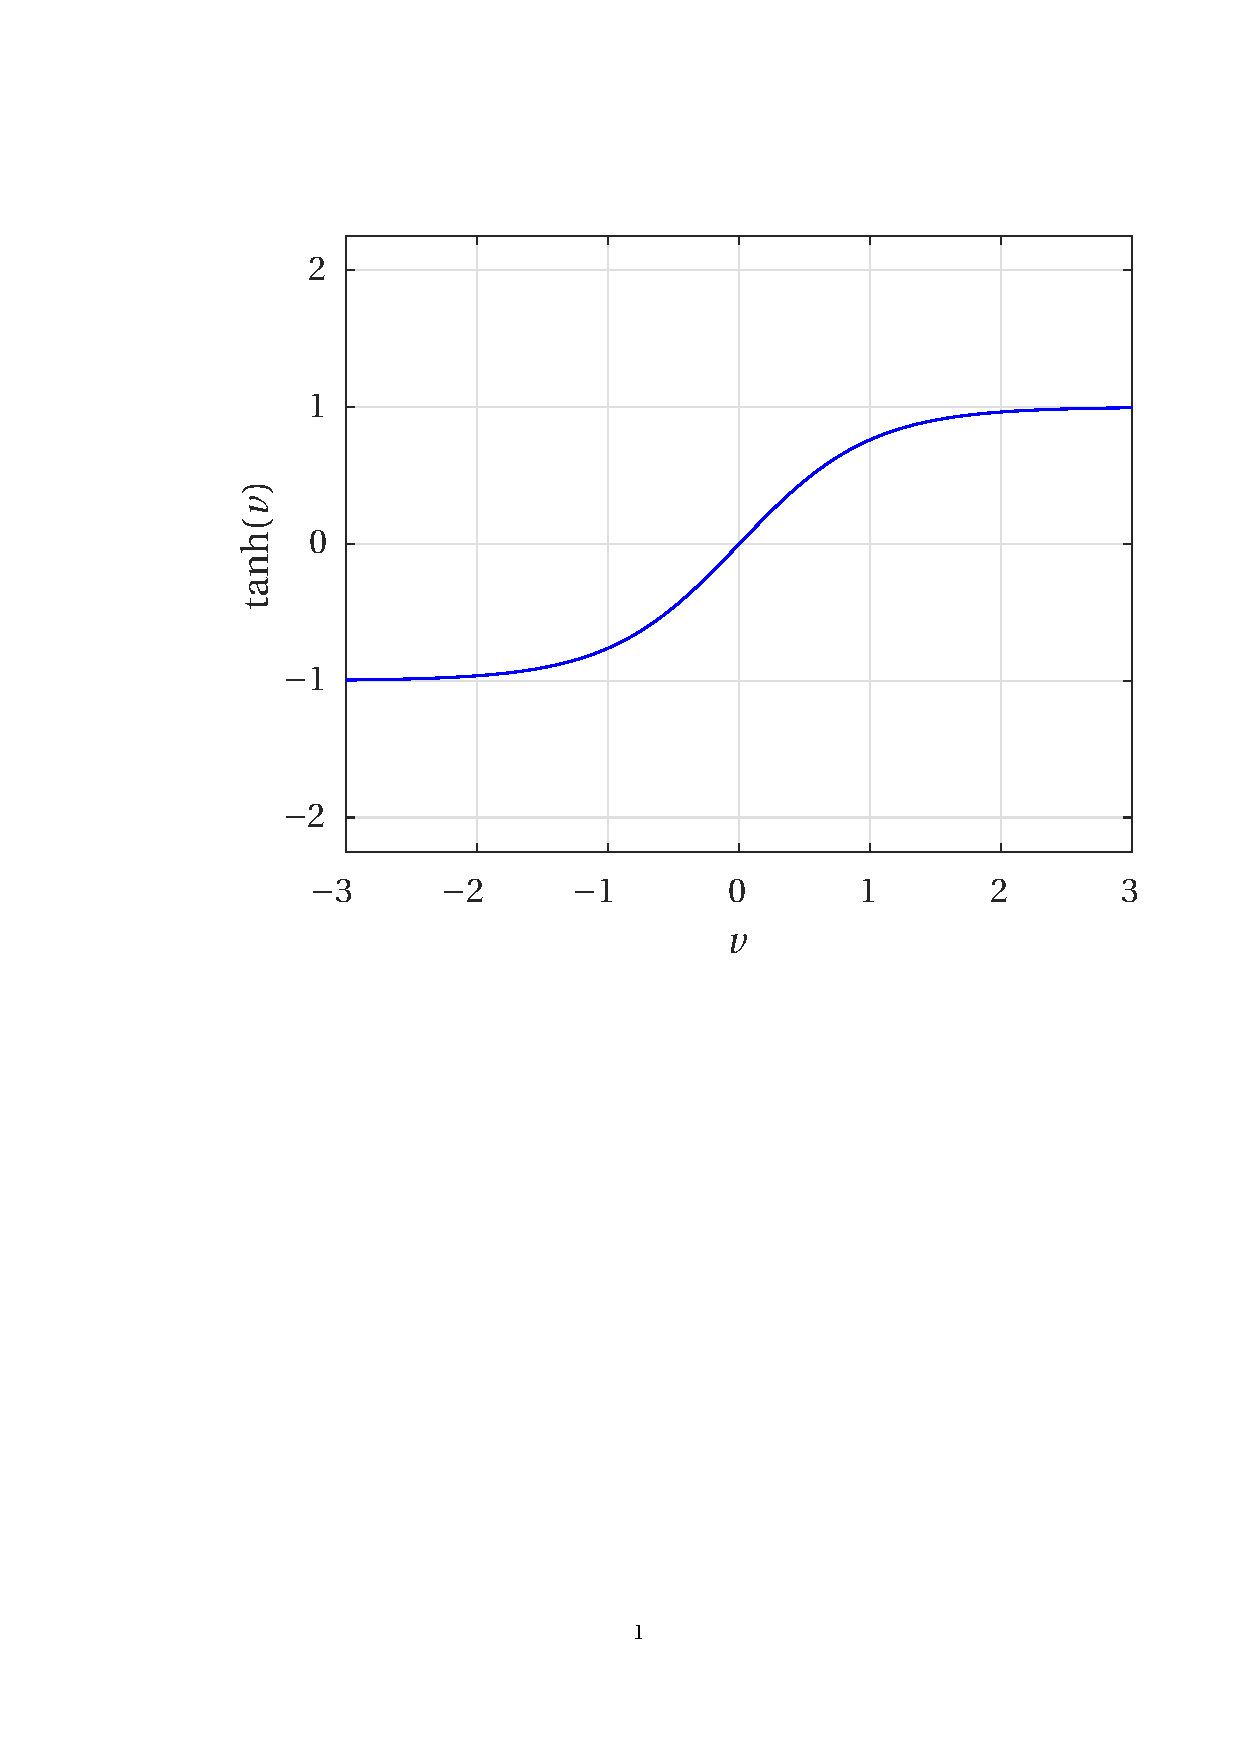
\includegraphics[scale = 0.44, trim = {2.5cm 13cm 1cm 3.5cm}, clip]{hyperbolic_tangent_bis}}
			
			\caption{Left: logistic function \eqref{eq:logistic} for three values of the parameter $T$; note that as $T$ decreases, the logistic function resemble the Heaviside function. Right: hyperbolic tangent.}
			\label{fig:activation-functions}
		\end{figure}
		
		\vspace*{0.3cm}
		
		\noindent \textbf{Feedforward neural network}. In a feedforward neural network, also called \emph{perceptron} \cite{Ros58}, neurons are arranged into \emph{layers}, with one \emph{input layer} of $M_I$ source neurons, $K$ \emph{hidden layers}, each one consisting of $H_k$ computing neurons, $k = 1, \, \ldots \, , K$, and an \emph{output layer} of $M_O$ computing neurons. As characteristic property, neurons in a layer can only be connected with neurons in the next layer towards the output layer. Then, an \emph{activation pattern} $\boldsymbol{p} \in \mathbb{R}^{M_I}$, supplied to the network through the source nodes in the first layer, provides the input signal for the neurons in the first hidden layer. For each hidden layer, its output signal gives the input pattern for the following layer. In this way, informations travel towards the last layer of the network, i.e., the output layer, whose outputs constitute the components of the overall output $\boldsymbol{q} \in \mathbb{R}^{M_O}$ of the network, response to the input pattern $\boldsymbol{p}$\footnote{Please note that while the output of a single neuron is denoted with the letter $y$, we use the letter $\boldsymbol{q}$ (bolded) to indicate the overall output of the network. Clearly, for the $j$-th output neuron the output $y_j$ coincides with the correspondent entry of $\boldsymbol{q}$, i.e., $q_j = y_j$, $j = 1, \, \ldots \, , M_O$.}. Hence, a feedforward network establish a map between the \emph{input space} $\mathbb{R}^{M_I}$ and the \emph{output space} $\mathbb{R}^{M_O}$. This makes this network architecture particularly suitable for, e.g., classification and continuous function approximation.
		
		Feedforward networks can be classified according to the number of hidden neurons they present, or, equivalently, the number of layers of trainable weights. Single-layer perceptrons (SLPs) just consist of the input and output layer; no hidden layers. Note that the layer which the name refers to is the output layer; the input layer is not accounted for since it does not perform any calculation. Despite their quite simple structure, the range of application of single-layer perceptrons is rather limited. Indeed, consider a binary input vector, supplied to an SLP provide with a unique output neuron, equipped with a binary activation function. The network acts then as a classifier, splitting the input space, i.e., the unit hypercube, by means of a hyperplane. Therefore, only \emph{linearly separable} data can be properly represented \cite{Kri}. On the other hand, the share of linearly separable sets decreases as the space dimension increases, making single-layer perceptrons seldom attractive.
		
		Conversely, multi-layer perceptrons (MLPs), providing at least one hidden layer, are universal function approximators, as stated by Cybenko \cite{Cyb88, Cyb89}. In detail:
		\begin{enumerate}[label=(\roman*)]
			\item a multi-layer perceptron with one layer of \emph{hidden neurons} and differentiable activation functions can approximate any \emph{continuous} function \cite{Cyb89};
			\label{cybenko-first-rule}
			\item a multi-layer perceptron with two layers of \emph{hidden neurons} and differentiable activation functions can approximate \emph{any function} \cite{Cyb88}.
			\label{cybenko-second-rule}
		\end{enumerate}
		Therefore, in many practical applications there is no reason to employ MLPs with more than two hidden layers. Considering again the binary classifier discussed above, one can represent any convex polygon by adding one hidden layer, and any arbitrary set by adding two hidden layers; further increasing the number of hidden neurons would not improve the representation capability of the network. However, we should point out that \ref{cybenko-first-rule} and \ref{cybenko-second-rule} do not give any practical advice on both the number of hidden neurons and the number of samples required to teach the network.
		
		An instance of a three-layer (i.e., two hidden layer plus the output layer) feedforward network is offered in Figure \ref{}. In this case, we have $M_I = 3$ input neurons (denoted with the letter $i$), $H_1 = H_2 = 6$ hidden neurons (letter $h$), and $M_O = 4$ output neurons (letter $o$). In particular, we point out that it represents an instance of a \emph{completely linked} perceptron, since each neuron is directly connected with all neurons in the following layer.
		
		Finally, let us just mention that, although we have previously stated that in a feedforward neural network a synapses can only connect pairs of neurons in contiguous layers, recent years have seen the development of different variants. For instance, \emph{shortcut connections} skip one or more layers, while \emph{lateral connections} takes place between neurons within the same layer. However, throughout this work we shall be faithful to the original definition of the perceptron.
				
		\vspace*{0.3cm}
		
		\noindent \textbf{Recurrent neural network}. In recurrent networks any neuron can bind with any other neuron, but autosynapses are forbidden, i.e., the output of a neuron can be input into the same neuron at the next time step. If each neuron is connected with all other neurons, then the network is said \emph{completely linked}. As a consequence, one can not distinguish neither input or output neurons any more: neurons are all equivalent. Then, the input of the network is represented by the initial \emph{network state}, which is the set of activation states for all neurons in the network. Similarly, the overall network output is given by the final network state. So, communication between a recurrent neural network and the surrounding environment takes place through the states of the neurons. Examples of recurrent networks are the Hopfield networks \cite{Hop82}, inspired by the behaviour of electrically charged particles within a magnetic field, and the self-organizing maps by Kohonen \cite{Koh98}, highly suitable for cluster detection.
		
		\vspace*{0.3cm}
		
		As mentioned in the introductory chapter, in this work we refer to neural networks for the approximation of the unknown map $\boldsymbol{\phi}$ between the parameters $\boldsymbol{\mu}$ of a parametrized partial differential equation, and the coefficients $\boldsymbol{\alpha}$ of the corresponding reduced basis solution. To accomplish this task, we rely on a collection of samples $\big\lbrace \boldsymbol{\mu}_i, \boldsymbol{\alpha}_i \big\rbrace_{i = 1}^{N_{tr}}$ generated through a high-fidelity model. Although a detailed explanation will be provided later in Chapter \ref{}, what is worth notice here is that we are concerned with a \emph{continuous function approximation} problem. Then, motivated by what previously said in the section, a multi-layer feedforward neural network turns out as the most suitable network architecture for our purposes. 
		
		We are now left to investigate the way the weights of a perceptron can be \emph{trained} to meet our purposes.
		
	\vspace*{0.3cm}
		
	\subsection{Training a multilayer feedforward neural network}
	\label{section:Training a multilayer feedforard neural network}
	
		As widely highlighted so far, the primary characteristic of a neural network lies in the capability to \emph{learn} from the environment, storing the acquired knowledge through the network internal parameters, i.e., the synaptic and bias weights. Learning is accomplished through a training process, during which the network is exposed to a collection of examples, called \emph{training patterns}. According to some performance measure, the weights are then adjusted by means of a well-defined set of rules. Therefore, a learning procedure is an \emph{algorithm}, typically iterative, modifying the neural network parameters to make it knowledgeable of the specific environment it operates in \cite{Hay05}. Specifically, this entails that after a successfull training, the neural network has to provide reasonable responses for unknown problems of the same class the network was acquainted with during training. This property is known as \emph{generalization} \cite{Kri}. 
		
		Training algorithms can be firstly classified based on the nature of the training set, i.e., the set of training patterns. We can then distinguish three \emph{learning paradigms}.
		
		\vspace*{0.3cm}
		
		\noindent \textbf{Supervised learning}. The training set consists of a collection of \emph{input patterns} (i.e., input vectors) $\big\lbrace \boldsymbol{p}_i \big\rbrace_{i = 1}^{N_{tr}}$, and corresponding desired responses $\big\lbrace \boldsymbol{t}_i \big\rbrace_{i = 1}^{N_{tr}}$, called \emph{teaching inputs}. Then, $\boldsymbol{t}_i$ is the output the neural network should desirably provide when it gets fed with $\boldsymbol{p}_i$. As we shall see, any training procedure aims to minimize (in some appropriate norm) the discrepancy between the \emph{desired} output $\boldsymbol{t}_i$ and the \emph{actual} output $\boldsymbol{q}_i$ given by the network as response to $\boldsymbol{p}_i$. 
		
		\vspace*{0.3cm}
		
		\begin{figure}[t]
			\center
			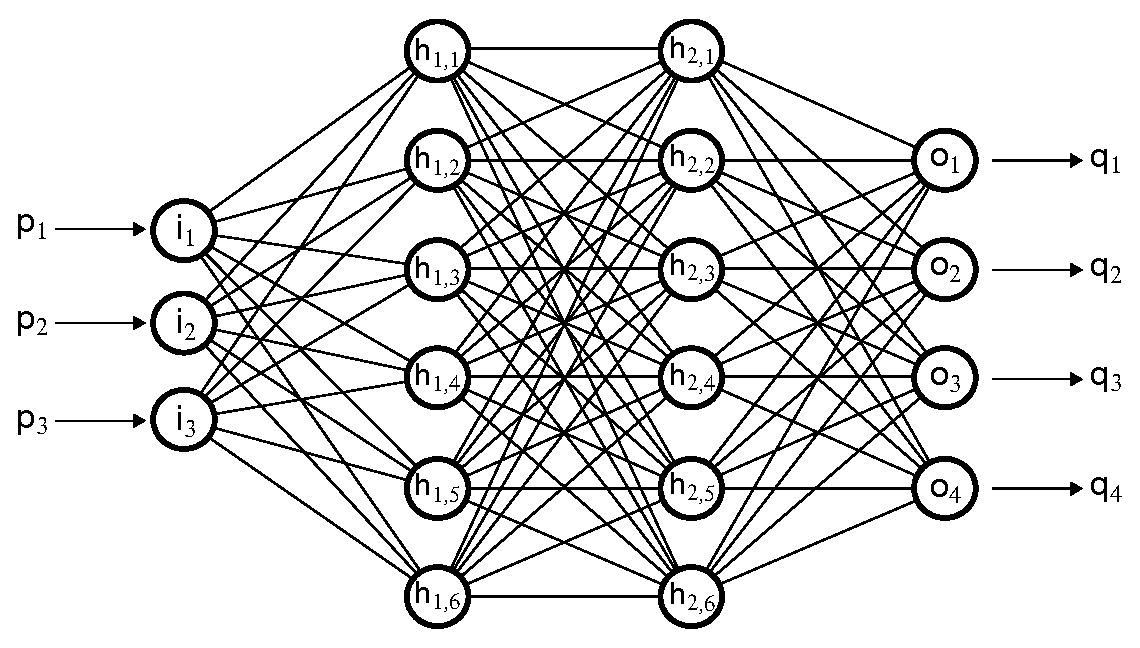
\includegraphics[scale = 0.6]{neural_network_bis.eps}
			
			\caption{A three-layer feedforward neural network, with $3$ input neurons, two hidden layers each one consisting of $6$ neurons, and $4$ output neurons. Within each connection, information flows from left to right.}
			\label{fig:neural-network}
		\end{figure}
		
		\noindent \textbf{Unsupervised learning}. Although supervised learning is a simple and intuitive paradigm, there exist many tasks which require a different approach to be tackled. Consider for instance a cluster detection problem. Due to lack of prior knowledge, rather than telling the neural network how it should behave in certain situations, one would like the neurons to \emph{independently} identify rules to group items. Therefore, a training pattern just consist of an input pattern. Since no desired output is provided, such a pattern is referred to as \emph{unlabeled}, as opposed to the \emph{labeled} examples involved in the supervised learning paradigm.
		
		\vspace*{0.3cm}
		
		\noindent \textbf{Reinforcement learning}. Reinforcement learning is the most plausible paradigm from a biological viewpoint. After the completion of a series of input patterns, the neural network is supplied with a boolean or a real saying whether the network is wrong or right. In the former case, the \emph{feedback} or \emph{reward} may also indicate to which extent the network is wrong \cite{Kri}. Conversely to the supervised and unsupervised paradigms, reinforcement learning focuses on finding a balance between exploration (of uncharted territory) and exploitation (of current knowledge). Hence, this paradigm particularly suits problems involving a trade-off between a long-term and a short-term reward \cite{KLM96}.
		
		\vspace*{0.3cm}
		
		Clearly, the choice of the learning paradigm is task-dependent. In particular, function approximation (i.e., what we are interested in) perfectly fits the \emph{supervised learning} paradigm. Indeed, consider the nonlinear unknown function $\boldsymbol{f}$,
		\begin{equation*}
			\begin{aligned}
				\boldsymbol{f} ~ : ~ & \mathbb{R}^{M_I} \hspace*{-0.3cm} && \rightarrow \mathbb{R}^{M_O} \\
								   & \boldsymbol{x} && \mapsto \boldsymbol{y} = \boldsymbol{f}(\boldsymbol{x}) \, ,
			\end{aligned}
		\end{equation*}
		and a set of labeled examples $\big\lbrace \boldsymbol{x}_i, \boldsymbol{y}_i \big\rbrace_{i = 1}^{N_{tr}}$. The task implies to approximate $\boldsymbol{f}$ over a domain $V \subset \mathbb{R}^{M_I}$ up to a user-defined tolerance $\epsilon$, i.e.,
		\begin{equation*}
			||\boldsymbol{F}(\boldsymbol{x}) - \boldsymbol{f}(\boldsymbol{x})|| < \epsilon \hspace*{0.3cm} \text{$\forall \boldsymbol{x} \in V$} \, ,
		\end{equation*}
		where $\boldsymbol{F} : \mathbb{R}^{M_I} \rightarrow \mathbb{R}^{M_O}$ is the actual input-output map established by the neural network, and $||\cdot||$ is some suitable norm on $\mathbb{R}^{M_O}$. Surely, as necessary condition the neural system must satisfy to well approximate $\boldsymbol{f}$ for each input in the domain $V$, the system should provide accurate predictions for the input patterns, i.e., 
		\begin{equation*}
			\boldsymbol{F}(\boldsymbol{x}_i) \approx \boldsymbol{y}_i \, , \hspace*{0.3cm} \text{$\forall i = 1, \, \ldots \, , N_{tr}$} \, .
		\end{equation*} 
		Then, we could train the network through a supervised learning algorithm, employing $\big\lbrace \boldsymbol{x}_i \big\rbrace_{i = 1}^{N_{tr}}$ as input patterns and $\big\lbrace \boldsymbol{y}_i \big\rbrace_{i = 1}^{N_{tr}}$ as teaching inputs. That is, 
		\begin{equation*}
			\text{$\boldsymbol{p}_i = \boldsymbol{x}_i$ and $\boldsymbol{t}_i = \boldsymbol{y}_i$,} \hspace*{0.3cm} \text{$\forall i = 1, \, \ldots \, , N_{tr}$.}
		\end{equation*}
		
		As defined in the first part of the section, a training algorithm involves:
		\begin{enumerate}[label=(\alph*)]
			\item a set of well-defined rules to modify the synaptic and bias weights;
			\label{a}
			\item a \emph{performance function}, quantifying the current level of knowledge of the surrounding environment.
			\label{b}
		\end{enumerate}
		Regarding \ref{a}, a plethora of weight updating techniques have been proposed in literature, sometimes tailored on specific applications. Nevertheless, most of them relies on the well-known Hebbian rule, proposed by Donal O. Hebb in 1949 \cite{Heb49}. Inspired by neurobiological considerations, the rule can be stated in a two-steps fashion \cite{Hay05}:
		\begin{enumerate}[label=(\roman*)]
			\item if two neurons on either side of a synapse (connection) are activated simultaneously (i.e., synchronously) then the strength of that synapse is selectively increased;
			\label{first-rule}
			\item if two neurons on either side of a synapse are activated asynchronously, then that synapse is selectively weakened (or eliminated).
			\label{second-rule}
		\end{enumerate}
		Actually, \ref{second-rule} was not included in the original statement; nevertheless, it provides a natural extension to \label{first-rule} \cite{Hay05}.
		In mathematical terms, consider the synapsis between a sending neuron $i$ and a target neuron $j$. Then, at the $t$-th iteration (also called \emph{epoch}) of the training procedure, the weight $w_{i,j}(t)$ of the connection $(i,j)$ is modified by the quantity
		\begin{equation}
			\label{eq:hebbian-rule}
			\Delta w_{i,j}(t) \sim \eta ~ y_i(t) ~ a_j(t) \, ,
		\end{equation}
		where $\eta > 0$ is the \emph{learning rate}, and we have exploited the fact that $y_i = a_i$ since the output function is usually represented as the identity. Hence, at the subsequent iteration $t+1$ the synaptic weight is simply given by
		\begin{equation}
			\label{eq:weight-update}
			w_{i,j}(t+1) = w_{i,j}(t) + \Delta w_{i,j}(t) \, .
		\end{equation}
		Many of the supervised learning rules proposed in literature, included the backpropagation of error derived later, can be recast in the following form, which turns out as a generalization of the Hebbian rule \eqref{eq:hebbian-rule} \cite{Kri}:
		\begin{equation}
			\label{eq:generalized-hebbian-rule}
			\Delta w_{i,j} = \eta ~ h(y_i,w_{i,j}) ~ g(a_j,t_j) \, ,
		\end{equation}
		with the functions $h$ and $g$ dependent on the specific learning rule, and $t_j$ the $j$-th component of the teaching input $\boldsymbol{t}$. Note that all variables involved in \eqref{eq:generalized-hebbian-rule} are supposed to be evaluated at time $t$, i.e., the correction $\Delta w_{i,j}$ is time-dependent. In addition, let us remark that \eqref{eq:generalized-hebbian-rule} represents a \emph{local} and \emph{interactive} mechanism, since it involves both and only the neurons at the end-points of the synapse.
		
		The second ingredient required to define a training algorithm is the performance or error function $E$. This function somehow measures the discrepancy between the neural network knowledge of the surrounding environment, and the actual state of the environment itself. In other terms, the larger the performance function, the farer the neural network representation of the world is from the actual reality, i.e., the farer we are from the application goal. Therefore, every learning rule aims to \emph{minimize} the performance $E$ as much as possible. For this purpose, $E$ should be intended as a scalar function of the free parameters, i.e., the weights, of the network, namely 
		\begin{equation}
			\label{eq:performance-function}
			E = E(\boldsymbol{w}) \in \mathbb{R} \, . 
		\end{equation}
		Recalling the notation and assumptions introduced in Definiton \ref{def:neural-network}, here $\boldsymbol{w} \in \mathbb{R}^{|\mathcal{V}|}$ is a vector collecting the weights $\big\lbrace w_{i,j} = w((i,j)) \big\rbrace_{(i,j) \in \mathcal{V}}$, with $\mathcal{V}$ the set of admissible connections in the network\footnote{Please note that while in Definiton \ref{def:neural-network} $\mathcal{V}$ denoted the set of all \emph{possible} connections, here $\mathcal{V}$ disregards those connections which are not consistent with the network topology in use. For instance, a feedforward neural network can not be endowed with connections oriented towards the input layer, then such connections will not be included in $\mathcal{V}$. In this way, we reduce the size of $\boldsymbol{w}$ - which is a practical advantage.}. Thus, Equation \eqref{eq:performance-function} implies that the point over the error surface reached at the end of a successful training process provides the \emph{optimal} configuration $\boldsymbol{w}_{opt}$ for the network.
		
		The steps a generic supervised training procedure should pursued are listed by Algorithms \ref{alg:online-learning} and \ref{alg:offline-learning} for online and offline learning, respectively. \emph{Online} learning means that the weights are updated after the exposition of the network to each training pattern. In other terms, each epoch involves only one training pattern. Conversely, in an \emph{offline} learning procedure the modifications are based on the entire training set, i.e., the weights are adjusted only after the network has been fed with all input patterns and the corresponding errors have been accumulated. Therefore, we should distinguish between the \emph{specific error} $E_{\boldsymbol{p}}(\boldsymbol{w})$, specific to the activation pattern $\boldsymbol{p}$, and the \emph{total error} $E(\boldsymbol{w})$ accounting for all specific errors, namely
		\begin{equation}
			\label{eq:accumulated-error}
			E(\boldsymbol{w}) = \sum_{\boldsymbol{p} \in P} E_{\boldsymbol{p}}(\boldsymbol{w}) \, ,
		\end{equation}
		with $P$ the training set. For instance, we could think of the specific error as the Mean Squared Error (MSE): 
		\begin{equation}
			\label{eq:mse}
			E_{\boldsymbol{p}}(\boldsymbol{w}) = \dfrac{1}{M_O} \sum_{j = 1}^{M_O} \left( t_{\boldsymbol{p},j} - q_{\boldsymbol{p},j} \right)^2 \, ,
		\end{equation}
		where we have added the subscript $\boldsymbol{p}$ to the components of the teaching input $\boldsymbol{t}$ and the actual output $\boldsymbol{q}$ to remark they refer to the input pattern $\boldsymbol{p}$. Accordingly, we could provide the following definition for the accumulated MSE:
		\begin{equation}
			\label{eq:accumulated-mse}
			E(\boldsymbol{w}) = \sum_{\boldsymbol{p} \in P} E_{\boldsymbol{p}}(\boldsymbol{w}) = \sum_{\boldsymbol{p} \in P} \dfrac{1}{M_O} \sum_{j = 1}^{M_O} \left( t_{\boldsymbol{p}_i,j} - q_{\boldsymbol{p}_i,j} \right)^2 \, .
		\end{equation}
				
		\vspace*{0.3cm}
		
		\begin{algorithm}[t]
			\begin{algorithmic}[1]
				\Require neural network $\left( \mathcal{N}, \, \mathcal{V}, \, \bg{w}_0 \right)$, training set $P = \big\lbrace \bg{p}_i, \, \bg{t}_i \big\rbrace_{i = 1}^{N_{tr}}$, 
				\Statex \hspace*{0.535cm} metric $d(\cdot,\cdot) ~ : ~ \mathbb{R}^{M_O} \times \mathbb{R}^{M_O} \rightarrow \mathbb{R}$, tolerance $\epsilon$, maximum number of epochs $T$
				\Ensure trained neural network $\left( \mathcal{N}, \, \mathcal{V}, \, \bg{w}_{opt} \right)$
				\vspace*{0.2cm}
				\State $t = 0$, $i = 1$, $k = 0$
				\State $\bg{w}(0) = \bg{w}_0$
				\While{$t < T$ and $k < N$}
					\State evaluate output vector $\bg{y}_{\bg{p}_i}(t)$, correspondent to input pattern $\bg{p}_i$
					\State $E_{\bg{p}_i}(\bg{w}(t))$ = $d(\bg{y}_{\bg{p}_i}(t), \, \bg{t}_1)$
					\If{$E_{\bg{p}_i}(\bg{w}(t)) < \epsilon$}
						\State $k = k + 1$
					\Else
						\State $k = 0$
						\State compute weight update $\Delta \bg{w}(t)$ based on $E_{\bg{p}_i}(\bg{w}(t))$
						\State $\bg{w}(t+1) = \bg{w}(t) + \Delta \bg{w}(t)$
					\EndIf
					\State $t = t+1$, $i = i \Mod N + 1$					
				\EndWhile		
				\State $\bg{w}_{opt} = \bg{w}(t)$
			\end{algorithmic}
			
			\caption{Backbone of any supervised online learning algorithm; note that the full procedure ends when all training patterns yield an error which is below a defined threshold.}
			\label{alg:online-learning}
		\end{algorithm}
		\begin{algorithm}[t]
			\begin{algorithmic}[1]
				\Require neural network $\left( \mathcal{N}, \, \mathcal{V}, \, \bg{w}_0 \right)$, training set $P = \big\lbrace \bg{p}_i, \, \bg{t}_i \big\rbrace_{i = 1}^{N_{tr}}$, 
				\Statex \hspace*{0.535cm} metric $d(\cdot,\cdot) ~ : ~ \mathbb{R}^{M_O} \times \mathbb{R}^{M_O} \rightarrow \mathbb{R}$, tolerance $\epsilon$, maximum number of epochs $T$
				\Ensure trained neural network $\left( \mathcal{N}, \, \mathcal{V}, \, \bg{w}_{opt} \right)$
				\vspace*{0.2cm}
				\State $t = 0$
				\State $\bg{w}(0) = \bg{w}_0$
				\State $E(\bg{w}(0))$ = \Call{OfflineError}{$\mathcal{N}$, $\mathcal{V}$, $\bg{w}(0)$, $P$, $d$}
				\While{$t < T$ and $E(\bg{w}(t)) > \epsilon$}
					\State compute weight update $\Delta \bg{w}(t)$ based on $E(\bg{w}(t))$
					\State $\bg{w}(t+1) = \bg{w}(t) + \Delta \bg{w}(t)$
					\State $E(\bg{w}(t+1))$ = \Call{OfflineError}{$\mathcal{N}$, $\mathcal{V}$, $\bg{w}(t+1)$, $P$, $d$}
					\State $t = t+1$					
				\EndWhile		
				\State $\bg{w}_{opt} = \bg{w}(t)$
				\vspace*{0.2cm}
				\Function{$E(\bg{w}) = $ OfflineError}{$\mathcal{N}$, $\mathcal{V}$, $\bg{w}$, $P$, $d$}
					\State $E(\bg{w}) = 0$
					\For{$i = 1, \, \ldots \, , N_{tr}$}
						\State evaluate output vector $\bg{y}_{\bg{p}_i}$, correspondent to input pattern $\bg{p}_i$
						\State $E(\bg{w}) = E(\bg{w}) + d(\bg{y}_{\bg{p}_i}, \, \bg{t}_i)$
					\EndFor
				\EndFunction
			\end{algorithmic}
			
			\caption{Backbone of any supervised offline learning algorithm; the procedure to compute the accumulated error is provided as well.}
			\label{alg:offline-learning}
		\end{algorithm}
		
		So far, we have not yet discussed how the update $\Delta w_{i,j}$ for the weight $w_{i,j}$ can be practically computed at each iteration. That is, we have still to rigourously define the functions $h$ and $g$ involved in the generalized Hebbian rule \eqref{eq:generalized-hebbian-rule}. Then, let us recall that any given operation carried out by the neural network can be thought as a point over the error surface $E(\boldsymbol{w})$. Therefore, to increase the performance of the network, we need to iteratively move toward a (local) minimum of the surface \cite{Hay05}. For this purpose, we may employ a \emph{steepest descent} technique, thus following the direction of the anti-gradient, i.e.,
		\begin{equation}
			\label{eq:antigradient}
			\Delta w_{i,j} = - \eta \dfrac{\partial E(\boldsymbol{w})}{\partial w_{i,j}} \, ,
		\end{equation}
		$\eta > 0$ being the learning rate, modulating the size of the step; its role will be clearer later in the chapter. Among the others, the \emph{backpropagation of error} \cite{MR86} is surely the most-known supervised, gradient-based training procedure for a multi-layer feedforward neural network whose neurons are equipped with a \emph{semi-linear}, i.e., continuous and differentiable, activation function\footnote{Therefore, backpropagation cannot apply with a binary activation function.}. The derivation of the backpropagation algorithm is provided in the following.
		
	\subsubsection{Backpropagation of error}
	\label{section:Backpropagation of error}
		
		Let us consider the generic synapse $(i,j)$ of a multi-layer feedforward neural network, connecting the \emph{predecessor} neuron $i$ with the \emph{successor} neuron $j$. As mentioned before, suppose both $i$ and $j$ present a semi-linear activation function. By widely exploiting the chain rule, the backpropagation of error provides an operative formula for the evaluation of the antigradient of the error function $E(\boldsymbol{w})$ in an arbitrary point $\boldsymbol{w}$, thus allowing to compute the update $\Delta w_{i,j}$ for the weight $w_{i,j}$ according to \eqref{eq:antigradient}. For this purpose, we shall need to distinguish whether the successor neuron $j$ is either an output or an inner neuron. To improve the clarity of the following mathematical derivation, we shall decorate any variable concerning a neuron with the subscript $\boldsymbol{p}$, thus to explicitly specify the input pattern $\boldsymbol{p}$ we refer to.
		
		Let $S = \big\lbrace s_1, \, \ldots \, , s_m \big\rbrace$ the set of $m$ neurons sending their output to $j$ through the synapses $\big\lbrace (s_1,j), \, \ldots \, , (s_m,j) \big\rbrace$. Recalling the definition \eqref{eq:accumulated-error} of the accumulated error, via the chain rule we can formulate the derivative of $E(\boldsymbol{w})$ with respect to the weight $w_{i,j}$ as follows:
		\begin{equation}
			\label{eq:bp-first-equation}
			\dfrac{\partial E(\boldsymbol{w})}{\partial w_{i,j}} = \sum_{\boldsymbol{p} \in P} \dfrac{\partial E_{\boldsymbol{p}}(\boldsymbol{w})}{\partial w_{i,j}} = \sum_{\boldsymbol{p} \in P} \dfrac{\partial E_{\boldsymbol{p}}(\boldsymbol{w})}{\partial u_{\boldsymbol{p},j}} \dfrac{\partial u_{\boldsymbol{p},j}}{\partial w_{i,j}} \, .
		\end{equation}
		Let us focus on the product
		\begin{equation}
			\label{eq:bp-second-equation}
			\dfrac{\partial E_{\boldsymbol{p}}(\boldsymbol{w})}{\partial u_{\boldsymbol{p},j}} \dfrac{\partial u_{\boldsymbol{p},j}}{\partial w_{i,j}}
		\end{equation}
		occurring in Equation \eqref{eq:bp-first-equation}. Assuming the propagation function be represented as the weighted sum, so that the net input is given by \eqref{eq:net-input}, the second factor in \eqref{eq:bp-second-equation} reads:
		\begin{equation}
			\label{eq:bp-third-equation}
			\dfrac{\partial u_{\boldsymbol{p},j}}{\partial w_{i,j}} = \dfrac{1}{\partial w_{i,j}} \left( \sum_{s \in S} w_{s,j} ~ y_{\boldsymbol{p},s} - \theta_j \right) = y_{\boldsymbol{p},i} \, .
		\end{equation}
		We then denote the opposite of the first term in \eqref{eq:bp-second-equation} by $\delta_{\boldsymbol{p},j}$, i.e.,
		\begin{equation}
			\label{eq:delta}
			\delta_{\boldsymbol{p},j} = - \dfrac{\partial E_{\boldsymbol{p}}(\boldsymbol{w})}{\partial u_{\boldsymbol{p},j}} \, .
		\end{equation} 
		$\delta_{\boldsymbol{p},j}$ is often referred to as the \emph{sensitivity} of the specific error $E_{\boldsymbol{p}}$ with respect to neuron $j$. Plugging \eqref{eq:delta} and \eqref{eq:bp-third-equation} into \eqref{eq:bp-first-equation}, then embedding the resulting equation into \eqref{eq:antigradient}, the weight update can be cast in the form:
		\begin{equation}
			\label{eq:bp-weight-update}
			\Delta w_{i,j} = \eta \sum_{\boldsymbol{p} \in P} \delta_{\boldsymbol{p},j} ~ y_{\boldsymbol{p},i} \, .
		\end{equation}
		We now proceed to derive an operative formula for $\delta_{\boldsymbol{p},j}$. Consider the case $j$ is an output neuron. Supposing a specific error of the form \eqref{eq:mse} and an identity output function, it follows: 
		\begin{equation}
			\label{eq:bp-fourth-equation}
			\begin{aligned}
				\delta_{\boldsymbol{p},j} & = - \dfrac{\partial E_{\boldsymbol{p}}(\boldsymbol{w})}{\partial y_{\boldsymbol{p},j}} ~ \dfrac{\partial y_{\boldsymbol{p},j}}{\partial u_{\boldsymbol{p},j}} \\
				& = - \dfrac{1}{\partial y_{\boldsymbol{p},j}} \dfrac{1}{M_O} \sum_{k = 1}^{M_O} \left( t_{\boldsymbol{p},k} - y_{\boldsymbol{p},k} \right)^2 ~ \dfrac{\partial a_{\boldsymbol{p},j}}{\partial u_{\boldsymbol{p},j}} \\
				& = \dfrac{2}{M_O} \left( t_{\boldsymbol{p},j} - y_{\boldsymbol{p},j} \right) ~ \dfrac{\partial f_{act}(u_{\boldsymbol{p},j})}{\partial u_{\boldsymbol{p},j}} \\
				& = \dfrac{2}{M_O} \left( t_{\boldsymbol{p},j} - y_{\boldsymbol{p},j} \right) ~ f'_{act}(u_{\boldsymbol{p},j}) \, .
			\end{aligned}
		\end{equation}
		It worths mention here that \eqref{eq:bp-fourth-equation} implies the derivative $f'_{act}$ of the activation function $f_{act}$ with respect to its argument. This motivates the requirement of a differentiable transfer function. 
		
		On the other hand, Equation \eqref{eq:bp-fourth-equation} does not apply when $j$ lies within an hidden layer. In fact, no teaching input is provided for an hidden neuron. In that case, let us denote by $R = \big\lbrace r_1, \, \ldots \, , r_n \big\rbrace$ the set of $n$ neurons receveing the output generated by $j$, i.e., the \emph{successors}. We then point out that the output of any neuron can directly affect only the neurons which receive the output itself, i.e., the successors \cite{Kri}. Hence: 
		\begin{equation}
			\label{eq:bp-fifth-equation}
			\begin{aligned}
				\delta_{\boldsymbol{p},j} & = \dfrac{\partial E_{\boldsymbol{p}}(\boldsymbol{w})}{\partial u_{\boldsymbol{p},j}} \\
				& = \dfrac{\partial E_{\boldsymbol{p}}(u_{\boldsymbol{p},r_1}, \, \ldots \, , u_{\boldsymbol{p},r_n})}{\partial u_{\boldsymbol{p},j}} \\
				& = \dfrac{\partial E_{\boldsymbol{p}}(u_{\boldsymbol{p},r_1}, \, \ldots \, , u_{\boldsymbol{p},r_n})}{\partial y_{\boldsymbol{p},j}} ~ \dfrac{\partial y_{\boldsymbol{p},j}}{\partial u_{\boldsymbol{p},j}} \\
				& = \sum_{k = 1}^{n} \dfrac{\partial E_{\boldsymbol{p}}}{\partial u_{\boldsymbol{p},r_k}} ~ \dfrac{\partial u_{\boldsymbol{p},r_k}}{\partial y_{\boldsymbol{p},j}} ~ \dfrac{\partial y_{\boldsymbol{p},j}}{\partial u_{\boldsymbol{p},j}} \, .
			\end{aligned}
		\end{equation}
		Applying the definition of sensitivity for neuron $r_k$, $k = 1, \, \ldots \, , n$, under the same assumptions of Equation \eqref{eq:bp-fourth-equation} we can further develop \eqref{eq:bp-fifth-equation}:
		\begin{equation}
			\label{eq:bp-sixth-equation}
			\begin{aligned}
			\delta_{\boldsymbol{p},j} & = \sum_{k = 1}^n \left( - \delta_{\boldsymbol{p},r_k} \right) ~ \dfrac{1}{\partial y_{\boldsymbol{p},j}} \left( \sum_{l = 1}^{m_k} w_{s_l,r_k} y_{\boldsymbol{p},s_l} - \theta_{r_k} \right) ~ \dfrac{\partial f_{act}(u_{\boldsymbol{p},j})}{\partial u_{\boldsymbol{p},j}} \\
			& = - \sum_{k = 1}^n \delta_{\boldsymbol{p},r_k} ~ w_{j,r_k} ~ f'_{act}(u_{\boldsymbol{p},j}) \, .
			\end{aligned}
		\end{equation}
		Here, we have supposed that $r_k$ receives input signals from $m_k$ neurons $\big\lbrace s_1, \, \ldots \, s_{m_k} \big\rbrace$.
		
		Let us now collect and summarize the results derived so far. At any iteration $t$ of the backpropagation learning algorithm, the weight $w_{i,j}(t)$ of a generic connection $(i,j)$ linking neuron $i$ with neuron $j$ is corrected by an additive quantity $\Delta w_{i,j}(t)$, i.e., 
		\begin{equation*}
			w_{i,j}(t+1) = w_{i,j}(t) + \Delta w_{i,j}(t) \, .
		\end{equation*}
		Assume the accumulated mean squared error \eqref{eq:accumulated-mse} as performance function. Understanding the dependence on time for the sake of clarity, the weight update $\Delta w_{i,j}$ reads:
		\begin{equation*}
			\Delta w_{i,j} = \eta \sum_{\boldsymbol{p} \in P} y_{\boldsymbol{p},i} ~ \delta_{\boldsymbol{p},j} \, ,
		\end{equation*}
		where $\eta > 0$, while $\delta_{\boldsymbol{p},j}$ is given by
		\begin{subnumcases}{\delta_{\boldsymbol{p},j} =}
			\label{eq:bp-inner-neuron}
		   	f'_{act}(u_{\boldsymbol{p},j}) \sum_{r \in R} \delta_{\boldsymbol{p},r} ~ w_{j,r} \, , & \text{if $j$ inner neuron} \, , \\
		   	\label{eq:bp-output-neuron}
			\dfrac{2}{M_O} f'_{act}(u_{\boldsymbol{p},j}) \left( t_{\boldsymbol{p},j} - y_{\boldsymbol{p},j} \right) \, , & \text{if $j$ output neuron} \, .
		\end{subnumcases}
				
		Some relevant remarks about the overall algorithm should be pointed out. First, observe that Equation \eqref{eq:bp-inner-neuron} defines $\delta_{\boldsymbol{p},j}$ for a hidden node $j$ by relying on neurons in the following layer, whereas Equation \eqref{eq:bp-output-neuron} only involves variables concerning the neuron (namely, $u_{\boldsymbol{p},j}$ and $y_{\boldsymbol{p},j}$) and the exact output $t_{\boldsymbol{p},j}$. Therefore, the coupled equations \eqref{eq:bp-inner-neuron}-\eqref{eq:bp-output-neuron} implicitly set the order in which the weights must be adjusted: starting from the output layer, update all the connections ending in that layer, then move backwards to the preceeding layer. In this way, the error is \emph{backpropagated} from the output down to the input, leaving traces in each layer of the network \cite{Kri, WH60}.
		
		The weight updating procedure detailed above corresponds to the offline version of the backpropagation of error, since it involves the total error $E$. On the other hand, the online algorithm readly comes from Equation \eqref{eq:bp-weight-update}: simply drop the summation over the elements of the training set $P$.
		
		Although intuitive and very promising, backpropagation of error suffers of all those drawbacks that are peculiar to gradient-based techniques. For instance, we may get stuck in a local minimum, whose level is possibly far from the global minimum of the error surface $E$. Furthermore, since the step size dictated by the gradient method is given by the norm of the gradient itself, minima close to steepest gradients are likely to be missed due to a large step size. This motivates the introduction in \eqref{eq:antigradient} of the learning rate $\eta \in (0,1]$, acting as a reducing factor and thus enabling a keener control on the descent. As suggested by Kriesel \cite{Kri}, in many applications reasonable values for $\eta$ lies in the range $[0.01,0.9]$. In particular, a time-dependent learning rate usually enables a more effective and more efficient training procedure. At the beginning of the process, when the network is far from the application goal, one often needs to span a large extent of the error surface, thus to identify a region of interest. Then, the learning rate should be large, i.e., close to $1$, thus to speed up the exploration. However, as we approach the optimal configuration, we may want to progressively reduce the learning rate, then the step size, to fine-tune the weights of the neural network. 
		
		Nevertheless, selecting an appropriate value for $\eta$ is still more an art than a science. Furthermore, for sigmoidal activations functions as the ones shown in Figure \ref{}, the derivative is close to zero far from the origin. This results in the fact that it becomes very difficult to move neurons away from the limits of the activation, which could extremely extend the learning time \cite{Kri}. Hence, different alternatives to backpropagation have been proposed in literature, either by modifying the original algorithm (as, e.g., the resilient backpropagation \cite{RB93} or the quickpropagation \cite{Fah88}), or pursuing a different numerical approach to the optimization problem. The latter class of algorithms includes the Levenberg-Marquardt algorithm, which we shall extensively use in our numerical tests.
				
		\subsubsection{Levenberg-Marquardt algorithm}
		\label{section:Levenberg-Marquardt algorithm}
		
		While backpropagation is a steepest descent algorithm, the Levenberg-Marquardt algorithm \cite{Mar63} is an approximation to the Newton's method \cite{Hag94}. As for backpropagation, the learning procedure is driven by the loss function $E = E(\boldsymbol{w})$, $\boldsymbol{w} \in |\mathcal{V}|$. Applying the Newton's method for the minimization of $E$, at each iteration the \emph{search direction} $\Delta \boldsymbol{w}$ is found by solving the following linear system:
		\begin{equation}
			\label{eq:newton}
			\nabla^2 E(\boldsymbol{w}) \Delta \boldsymbol{w} = - \nabla E(\boldsymbol{w}) \, ,
		\end{equation}
		where $\nabla E(\boldsymbol{w})$ and $\nabla^2 E(\boldsymbol{w})$ denotes, respectively, the gradient vector and the Hessian matrix of $E$ with respect to its argument $\boldsymbol{w}$. Assume now that the loss function is represented as the accumulated mean squared error, 
		\begin{equation}
			\label{eq:accumulated-mse-bis}
			E(\boldsymbol{w}) = \sum_{\boldsymbol{p} \in P} \dfrac{1}{M_O} \sum_{j = 1}^{M_O} \left( t_{\boldsymbol{p},j} - y_{\boldsymbol{p},j} \right)^2 = \sum_{\boldsymbol{p} \in P} \dfrac{1}{M_O} \sum_{j = 1}^{M_O} e_{\boldsymbol{p},j}(\boldsymbol{w})^2 \, ;
		\end{equation}
		with $e_{\boldsymbol{p},j}$ the $j$-th component of the error vector $\boldsymbol{e}_{\boldsymbol{p}} = \boldsymbol{t}_{\boldsymbol{p}} - \boldsymbol{y}_{\boldsymbol{p}}$ corresponding to the input pattern $\boldsymbol{p}$. Then, introducing the Jacobian $J_{\boldsymbol{p}}$ of the specific error vector $\boldsymbol{e}_{\boldsymbol{p}}$ with respect to $\boldsymbol{w}$, i.e., 
		\begin{equation}
			\label{eq:jacobian}
			J_{\boldsymbol{p}}(\boldsymbol{w}) = 
			\begin{bmatrix}
				\vspace*{0.2cm}
				\hspace*{-0.3cm} & \dfrac{\partial e_{\boldsymbol{p},1}}{\partial w_1} & \dfrac{\partial e_{\boldsymbol{p},1}}{\partial w_2} & \ldots & \dfrac{\partial e_{\boldsymbol{p},1}}{\partial w_{|\mathcal{V}|}} \\
				\vspace*{0.2cm}
				\hspace*{-0.3cm} & \dfrac{\partial e_{\boldsymbol{p},2}}{\partial w_1} & \dfrac{\partial e_{\boldsymbol{p},2}}{\partial w_2} & \ldots & \dfrac{\partial e_{\boldsymbol{p},2}}{\partial w_{|\mathcal{V}|}} \\
				\vspace*{0.2cm}
				\hspace*{-0.3cm} & \vdots & \vdots & \ddots & \vdots \\
				\hspace*{-0.3cm} & \dfrac{\partial e_{\boldsymbol{p},M_O}}{\partial w_1} & \dfrac{\partial e_{\boldsymbol{p},M_O}}{\partial w_2} & \ldots & \dfrac{\partial e_{\boldsymbol{p},M_O}}{\partial w_{|\mathcal{V}|}}
			\end{bmatrix}
			\in \mathbb{R}^{M_O \times |\mathcal{V}|}
		\end{equation}
		simple computations yield:
		\begin{equation}
			\label{eq:gradient}
			\nabla E(\boldsymbol{w}) = \sum_{\boldsymbol{p} \in P} \dfrac{2}{M_0} J_{\boldsymbol{p}}(\boldsymbol{w})^T \boldsymbol{e}_{\boldsymbol{p}} \in \mathbb{R}^{|\mathcal{V}|}
		\end{equation}
		and
		\begin{equation}
			\label{eq:hessian}
			\nabla^2 E(\boldsymbol{w}) = \sum_{\boldsymbol{p} \in P} \dfrac{2}{M_O} \left[ J_{\boldsymbol{p}}(\boldsymbol{w})^T J_{\boldsymbol{p}}(\boldsymbol{w}) + S(\boldsymbol{w}) \right] \in \mathbb{R}^{|\mathcal{V}| \times |\mathcal{V}|} \, ,
		\end{equation}
		with
		\begin{equation*}
			S(\boldsymbol{w}) = \sum_{\boldsymbol{p} \in P} \dfrac{2}{M_O} \sum_{j = 1}^{M_O} e_{\boldsymbol{p},j} \nabla^2 e_{\boldsymbol{p},j} \, .
		\end{equation*}
		Assuming $S(\boldsymbol{w}) \approx 0$, inserting \eqref{eq:gradient} and \eqref{eq:hessian} into \eqref{eq:newton} we get the linear system
		\begin{equation}
			\label{eq:newton-quadratic-function}
			\left[ \sum_{\boldsymbol{p} \in P} J_{\boldsymbol{p}}(\boldsymbol{w})^T J_{\boldsymbol{p}}(\boldsymbol{w}) \right] \Delta \boldsymbol{w} = - \sum_{\boldsymbol{p} \in P} J_{\boldsymbol{p}}(\boldsymbol{w})^T \boldsymbol{e}_{\boldsymbol{p}}(\boldsymbol{w}) \, .
		\end{equation} 
		The Levenberg-Marquardt modification to the Newton's method reads \cite{Hag94, Mar63}:
		\begin{equation}
			\label{eq:levenberg-marquardt}
			\left[ \sum_{\boldsymbol{p} \in P} J_{\boldsymbol{p}}(\boldsymbol{w})^T J_{\boldsymbol{p}}(\boldsymbol{w}) + \mu I \right] \Delta \boldsymbol{w} = - \sum_{\boldsymbol{p} \in P} J_{\boldsymbol{p}}(\boldsymbol{w})^T \boldsymbol{e}_{\boldsymbol{p}}(\boldsymbol{w}) \, ,
		\end{equation}
		with $\mu \geq 0$ and $I$ the identity matrix of size $|\mathcal{V}| \times |\mathcal{V}|$. Note that if $\mu = 0$ we recover the Newton's method \eqref{eq:newton-quadratic-function}, while for $\mu \gg 1$ the search direction $\Delta \boldsymbol{w}$ approaches the antigradient of $E$, i.e., we recover the backpropagation algorithm. Then, the Levenberg-Marquardt algorithm can be seen as an interpolation between the Newton's method and the steepest descent method, aiming to retain the advantages of both techniques.
		
		The Levenberg-Marquardt training algorithm proceeds as follows. At each epoch $t$ of the training procedure, we solve the (potentially large) linear system \eqref{eq:levenberg-marquardt}. Whenever the step $\Delta \boldsymbol{w}(t)$ leads to a reduction in the performance function, i.e., $E(\boldsymbol{w}(t) + \Delta \boldsymbol{w}(t)) < E(\boldsymbol{w}(t))$, the parameter $\mu$ is reduced by a factor $\beta > 1$. Conversely, if $E(\boldsymbol{w}(t) + \Delta \boldsymbol{w}(t)) > E(\boldsymbol{w}(t))$ the parameter is multiplied by the same factor $\beta$. This reflects the idea that far from the actual minimum we should prefer the gradient method to the Newton's method, since the latter may diverge. Yet, once in a neighborhood of the minimum, we switch to the Newton's method so to exploit its faster convergence \cite{Mar63}.
		
		The key step in the algorithm is the computation of the Jacobian $J_{\boldsymbol{p}}(\boldsymbol{w})$ for each training vector $\boldsymbol{p}$. Suppose that the $k$-th element $w_k$ of $\boldsymbol{w}$ represents the weight $w_{i,j}$ of the connection $(i,j)$, for some $i$ and $j$, with $1 \leq i \, , j \leq |\mathcal{N}|$. Then, the $(h,k)$-th entry of $J_{\boldsymbol{p}}(\boldsymbol{w})$ is given by:
		\begin{equation}
			\label{eq:jacobian-entry}
			\dfrac{\partial e_{\boldsymbol{p},h}}{\partial w_k} = \dfrac{\partial e_{\boldsymbol{p},h}}{\partial w_{i,j}} \, , \hspace*{0.3cm} 1 \leq h \leq M_O \, , 1 \leq k \leq |\mathcal{V}| \, .
		\end{equation}
		We recognize that the derivative on the right-hand side of Equation \eqref{eq:jacobian-entry} is intimately related with the gradient of the performance function. Therefore, we can follow the very same steps performed to derive the backpropagation, namely:
		\begin{equation}
			\label{eq:jacobian-entry-equation}
			\begin{aligned}
				\dfrac{\partial e_{\boldsymbol{p},h}}{\partial w_{i,j}} & = \dfrac{\partial e_{\boldsymbol{p},h}}{\partial u_{\boldsymbol{p},j}} ~ \dfrac{\partial u_{\boldsymbol{p},j}}{\partial w_{i,j}} \\[0.1cm]
				& = \dfrac{\partial e_{\boldsymbol{p},h}}{\partial y_{\boldsymbol{p},j}} ~ \dfrac{\partial y_{\boldsymbol{p},j}}{\partial u_{\boldsymbol{p},j}} ~ \dfrac{\partial u_{\boldsymbol{p},j}}{\partial w_{i,j}} \\[0.1cm]
				& = \dfrac{\partial e_{\boldsymbol{p},h}}{\partial y_{\boldsymbol{p},j}} ~ f'_{act}(u_{\boldsymbol{p},j}) ~ y_{\boldsymbol{p},i} \\
				& = \delta_{\boldsymbol{p},h,j} ~ y_{\boldsymbol{p},i} \, ,
			\end{aligned}
		\end{equation} 
		with
		\begin{equation}
			\label{eq:levenberg-marquardt-delta}
			\delta_{\boldsymbol{p},h,j} := - \dfrac{\partial e_{\boldsymbol{p},h}}{\partial u_{\boldsymbol{p},j}} = - \dfrac{\partial e_{\boldsymbol{p},h}}{\partial y_{\boldsymbol{p},j}} ~ f'_{act}(u_{\boldsymbol{p},j}) \, .
		\end{equation}
		For the computation of the derivative $\partial e_{\boldsymbol{p},h} ~ / ~ \partial y_{\boldsymbol{p},j}$ occurring in \eqref{eq:levenberg-marquardt-delta}, further assume that within the set of neurons $\mathcal{N}$ items are ordered such that the output neurons come first, i.e.,
		\begin{equation*}
			\text{$j$ output neuron \hspace*{0.2cm} $\Leftrightarrow$ \hspace*{0.2cm} $1 \leq j \leq M_O$} \, .
		\end{equation*} 
		We can then distinguish three cases:
		\begin{enumerate}[label=(\roman*)]
			\item $j$ output neuron, $j = h$: since $e_{\boldsymbol{p},h} = e_{\boldsymbol{p},j} = t_{\boldsymbol{p},j} - y_{\boldsymbol{p},j}$, then 
			\begin{equation}
				\label{eq:jacobian-first-case}
				\dfrac{\partial e_{\boldsymbol{p},h}}{\partial y_{\boldsymbol{p},j}} = -1 \, ;
			\end{equation}
			\item $j$ output neuron, $j \neq h$: the output of an output neuron can not influence the signal fired by another output neuron, hence 
			\begin{equation}
				\label{eq:jacobian-second-case}
				\dfrac{\partial e_{\boldsymbol{p},h}}{\partial y_{\boldsymbol{p},j}} = 0 \, ;
			\end{equation}
			\item $j$ inner neuron: letting $R$ be the set of successors of $j$, similarly to \eqref{eq:bp-sixth-equation} the chain rule yields
			\begin{equation}
				\label{eq:jacobian-third-case}
				\dfrac{\partial e_{\boldsymbol{p},h}}{\partial y_{\boldsymbol{p},j}} = \sum_{r \in R} \dfrac{\partial e_{\boldsymbol{p},h}}{\partial u_{\boldsymbol{p},r}} ~ \dfrac{\partial u_{\boldsymbol{p},r}}{\partial y_{\boldsymbol{p},j}} = - \sum_{r \in R} \delta_{\boldsymbol{p},h,r} ~ w_{j,r} \, .
			\end{equation}
		\end{enumerate}
		
		Ultimately, at any iteration of the learning algorithm the entries of the Jacobian matrix $J_{\boldsymbol{p}}$ are given by
		\begin{equation*}
			\dfrac{\partial e_{\bg{p},h}}{\partial w_k} = \delta_{\boldsymbol{p},h,j} ~ y_{\boldsymbol{p},i} \, , \hspace*{0.3cm} 1 \leq h \leq M_O \, , 1 \leq k \leq |\mathcal{V}| \, , \text{$w_k = w_{i,j}$ for some $i$ and $j$} \, ,
		\end{equation*}
		with
		\begin{subnumcases}{\delta_{\boldsymbol{p},h,j} =}
			\label{eq:levenberg-marquardt-inner-neuron}
		   	f'_{act}(u_{\boldsymbol{p},j}) \sum_{r \in R} \delta_{\boldsymbol{p},h,r} ~ w_{j,r} \, , & \text{if $j$ inner neuron} \, , \\
		   	\label{eq:levenberg-marquardt-output-neuron}
			f'_{act}(u_{\boldsymbol{p},j}) \delta_{jh}^K \, , & \text{if $j$ output neuron} \, ,
		\end{subnumcases}
		where $\delta_{jh}^K$ is the Kronecker delta. The steps to be performed at each iteration of the Levenberg-Marquardt algorithm are summarized in Algorithm \ref{alg:levenberg-marquardt}.
		
		Let us finally remark that a trial and error approach is still required to find satisfactory values for $\mu$ and $\beta$; as proposed in \cite{Mar63}, a good starting point may be $\mu = 0.01$, with $\beta = 10$. Moreover, the dimension of the system \eqref{eq:levenberg-marquardt} increases nonlinearly with the number of neurons in the network, making the Levenberg-Marquardt algorithm poorly efficient for large networks \cite{Hag94}. However, it is more efficient than backpropagation for networks with a few hundreads of connections, besides producing much more accurate results. We shall gain further insights into this topic in Chapter \ref{}.
		
		\begin{algorithm}[H]
			\begin{algorithmic}[1]
				\Function{$\left[ \bg{w} + \Delta \bg{w}, \, E(\bg{w} + \Delta \bg{w}), \, \mu \right]$ = LMiteration}{$\mathcal{N}$, $\mathcal{V}$, $\bg{w}$, $P$, $E(\bg{w})$, $d$, $\mu$}
					\State $\beta = 10$
					\For{$i = 1, \, \ldots \, , N_{tr}$}
						\State evaluate output vector $\bg{y}_{\bg{p}_i}$, correspondent to input pattern $\bg{p}_i$
						\State $\bg{e}_{\bg{p}_i} = \bg{y}_{\bg{p}_i} - \bg{t}_{\bg{p}_i}$
						\For{$h = 1, \, \ldots \, , M_0$, $k = 1, \, \dots \, , |\mathcal{V}|$}
							\State compute $\left( J_{\bg{p}_i} \right)_{h,k}$ according to \eqref{eq:jacobian-entry-equation}, \eqref{eq:levenberg-marquardt-inner-neuron} and \eqref{eq:levenberg-marquardt-output-neuron} 
						\EndFor
					\EndFor
					\State assemble and solve $\left[ \sum_{i = 1}^{N_{tr}} J_{\bg{p}_i}^T J_{\bg{p}_i} + \mu I \right] \Delta \boldsymbol{w} = - \sum_{i = 1}^{N_{tr}} J_{\bg{p}_i}^T \boldsymbol{e}_{\bg{p}_i}$
					\State $E(\bg{w} + \Delta \bg{w})$ = \Call{OfflineError}{$\mathcal{N}$, $\mathcal{V}$, $\bg{w} + \Delta \bg{w}$, $P_{tr}$, $d$}
					\If{$E(\bg{w} + \Delta \bg{w}) < E(\bg{w})$}
						\State $\mu = \mu / \beta$
					\Else
						\State $\mu = \mu * \beta$
					\EndIf 
				\EndFunction
			\end{algorithmic}
			
			\caption{An iteration of the Levenberg-Marquardt training algorithm.}
			\label{alg:levenberg-marquart}
		\end{algorithm}
						
	\subsection{Practical considerations on the design of artificial neural networks}
	\label{section:Practical considerations on the design of artificial neural networks}
	
		We conclude this introductory chapter on neural networks by discussing the major concerns regarding their design and implementation, mainly focusing on multi-layer perceptrons. As we shall see, most of these issues are still open questions in many research fields, and as such they should be tackled pursuing a \emph{trial-and-error} approach.
		
		In Section \ref{section:Network topologies}, we reported two fundamental results (\ref{cybenko-first-rule} and \ref{cybenko-second-rule}) promoting three-layers feedforward neural networks as universal function approximators. Yet, these statements do not provide any information regarding the number of neurons and training patterns required to approximate a function up to a desired level of uncertainty. In other terms, \ref{cybenko-first-rule} and \ref{cybenko-second-rule} are not operative, and therefore one has to rely on emprirical considerations and greedy approaches in the design and training of a neural network.  
		
		Clearly, the larger the training set, the better, and one could perform a sensitivity analysis on the amount of teaching inputs required to get satisfactory predictions. However, in real-life applications training data often come from an external source of information, on which we do not have any influence, and as a result the number of available teaching patterns is fixed. A relevant example is provided by recommender systems, which seek to build a predictive model based on a user's past behaviour (e.g., the items he/she has purchased) and similar choices made by other users. 
				
		The critical point for any network paradigm, designed either for continuous regression, classification or cluster-detection, is the choice of the right number of neurons it should be equipped with. As a rule of thumb, the network should feature as \emph{few} free parameters as possible but as many as \emph{necessary} \cite{Kri}. In this respect, recall that the computing and processing power of a network is determined by its neurons, while the weighted synapses represent the information storage. Then, too few neurons (i.e., synapses) do not endow the network with the necessary representation capability, leading to poor results, i.e., large values for the performance function. On the other hand, an oversized network would rather precisely align with the teaching inputs, but is likely to fail on patterns it has not been exposed to during the training. Indeed, being the degrees of freedom of the underlying problem fewer than the network paremeters, the latter can be tuned to lower the error function at will. In other words, once the training phase is over the system has successfully \emph{memorized} the training patterns but is not capable of \emph{generalizing} what it has learnt to similar (yet different) situations. In this circumstance, we say that the network \emph{overfits} the training data. 
		
		In the decades, many expedients have been proposed to avoid overfitting. For instance, one could alter the data through additive (white) noise, thus preventing the network to perfectly fit the training set. Another well-known practice is \emph{regularization}, which consists in correcting the error function by a regularizing term $L(\bg{\mu})$, namely
		\begin{equation*}
			E(\bg{w}) + \lambda L(\bg{w}) \, .
		\end{equation*}
		Here, $L$ is a functional increasing with the components of $\bg{w}$, thus penalizing large values for the weights, and so preventing the network from heavily relying on individual data points \cite{Mat16}. The positive coefficient $\lambda$ tunes the level of regularization introduced in the model: for $\lambda = 0$, we recover the original model, while for $\lambda \gg 1$ we sacrifice the performance on the training dataset for the sake of a more flexible system. As typical in neural networks, a suitable value for $\lambda$ has to be found empirically. 
		
		In our numerical experiments, overfitting is prevented upon resorting to \emph{cross-validation} combined with an \emph{early stopping} technique \cite{Koh95}. Data are split in three subsets: \emph{training}, \emph{validation}, and \emph{testing} data sets, denoted respectively by $P_{tr}$, $P_{va}$ and $P_{te}$. The former consists of data which are actually used to train the network. Specifically, in the Levenberg-Marquardt algorithm these data are used to build up the linear system \eqref{eq:levenberg-marquardt} yielding the weights and biases update $\Delta \bg{w}$. Whereas, validation samples are used to monitor the error performed by the model \emph{during} the training, but are not involved in the training itself. Finally, the testing data set is used to assess the performance of the system once the learning phase is over, and it is thus useful to compare different models, e.g., neural networks with different number of layers and/or neurons per layer \cite{Mat16}. For further details on the way such subsets have been generated for our test cases, we refer the reader to Chapter \ref{}.
		
		At the beginning of the learning stage, the error on both the training and validation data set typically decreases. However, while the error yielded by the training samples should keep lowering as time advances (provided a well-chosen minimization technique), at a certain point the validation error may start increasing, meaning that the network is likely to overfit the data. Therefore, we \emph{early stop} the procedure whenever the validation error keeps rising up for $K_{ea}$ consecutive iterations. The optimal configuration $\bg{w}_{opt}$ is then that one yielding the minimum of the validation (and not the training) error curve.
		
		Once in possession of an effective training procedure, one can basically pursue two different yet complementary strategies to determine a suitable number of neurons for a given application:
		\begin{enumerate}[label=(\alph*)]
			\item moving from a (relative) small amount of neurons, progressively augment the size of the network until the error on the test data set starts increasing;
			\item consider a sufficiently large number of neurons, then possibly adopt a \emph{pruning} strategy (e.g., the Optimal Brain Surgeon technique proposed by Hassibi \& Stork \cite{OBS}) to iteratively remove the \emph{less relevant} connection, erasing a neuron whenever it gets isolated from the rest of the network.
		\end{enumerate}
		As we shall explain in Chapter \ref{}, in this work we resort to the first approach for the sake of implementation-wise convenience. In particular, we first consider perceptrons with a single hidden layer, and we then add another computing layer whenever necessary\footnote{Recall that for perceptrons equipped with differential activation functions, two hidden layers are sufficient to approximate \emph{any} function.}
		
		Lastly, let us point out that the final network configuration resulting from any learning strategy is affected by the initial values assigned to the synaptic and bias weights. As a good practice, the weights should be initialized with random values averaging zero. In this respect, a random uniform sampling over $[-0.5,0.5]$ or a standard Gaussian distribution may be adequate choices. Then, to limit the dependence of the results on the initial configuration $\bg{w}_0$, we train each network topology several times, say $K_{mr}$, employing different $\bg{w}_0^k$, $k = 1, \, \ldots \, , K_{mr}$, finally keeping the configuration yielding the minimum error on the test data set. This approach is usually referred to as \emph{multiple-restarting}. The definitive training procedure used in this project, based on the Levenberg-Marquardt algorithm and keeping into consideration all the observations made in this section, is given in Algorithm \ref{alg:offline-learning-complete}.
								
		\begin{algorithm}[H]	
			\begin{algorithmic}[1]
				\Require neural network $\left( \mathcal{N}, \, \mathcal{V} \right)$, training set $P_{tr} = \big\lbrace \bg{p}_i, \, \bg{t}_i \big\rbrace_{i = 1}^{N_{tr}}$, validation set $P_{va} = \big\lbrace \bg{p}_i, \, \bg{t}_i \big\rbrace_{i = 1}^{N_{va}}$,
				\Statex \hspace*{0.535cm} testing set $P_{te} = \big\lbrace \bg{p}_i, \, \bg{t}_i \big\rbrace_{i = 1}^{N_{te}}$, metric $d(\cdot,\cdot) ~ : ~ \mathbb{R}^{M_O} \times \mathbb{R}^{M_O} \rightarrow \mathbb{R}$, 
				\Statex \hspace*{0.535cm} number of restarts $K_{ms}$, tolerance $\epsilon$, maximum number of epochs $T$,
				\Statex \hspace*{0.535cm} maximum number of consecutive iterations with an increasing validation error $K_{ea}$
				\Ensure trained neural network $\left( \mathcal{N}, \, \mathcal{V}, \, \bg{w}_{opt} \right)$
				\vspace*{0.2cm}
				\State $E_{opt} = \infty$
				\For{$j = 1, \, \ldots \, , K_{ms}$}
					\State $t = 0$, $k = 0$, $\mu = 0.01$
					\State randomly generate $\bg{w}(0)$
					\State $E_{tr}(\bg{w}(0))$ = \Call{OfflineError}{$\mathcal{N}$, $\mathcal{V}$, $\bg{w}(0)$, $P_{tr}$, $d$}
					\While{$t < T$ and $E_{tr}(\bg{w}(t)) > \epsilon$ and $k < K_{ea}$}
						\State $\left[ \bg{w}(t+1), \, E_{tr}(\bg{w}(t+1)), \, \mu \right]$ = \Call{LMiteration}{$\mathcal{N}$, $\mathcal{V}$, $\bg{w}(t)$, $P_{tr}$, $E(\bg{w}(t))$, $d$, $\mu$}
						\State $E_{va}(\bg{w}(t+1))$ = \Call{OfflineError}{$\mathcal{N}$, $\mathcal{V}$, $\bg{w}(t+1)$, $P_{va}$, $d$}
						\If{$E_{va}(\bg{w}(t+1)) > E_{va}(\bg{w}(t))$}
							\State $k = k + 1$
						\Else
							\State $k = 0$
						\EndIf
						\State $t = t+1$					
					\EndWhile		
					\State $\bg{w}_{opt}^{(j)} = \bg{w}(t-k)$
					\State $E_{te} \big( \bg{w}_{opt}^{(j)} \big)$ = \Call{OfflineError}{$\mathcal{N}$, $\mathcal{V}$, $\bg{w}_{opt}^{(j)}$, $P_{te}$, $d$}
					\If{$E_{te} \big( \bg{w}_{opt}^{(j)} \big) < E_{opt}$}
						\State $\bg{w}_{opt} = \bg{w}_{opt}^{(j)}$
						\State $E_{opt} = E_{te} \big( \bg{w}_{opt}^{(j)} \big)$
					\EndIf
				\EndFor
				
			\end{algorithmic}
			
			\caption{The complete training algorithm adopted in our numerical tests.}
			\label{alg:offline-learning-complete}
		\end{algorithm}
		
		

	\chapter{Reduced basis methods for nonlinear partial differential equations}
	\label{chapter:Reduced Basis method for nonlinear partial differential equations}
			
		In this chapter, we combine a reduced basis (RB) method with neural networks for the efficient resolution of parametrized nonlinear partial differential equations (PDEs) defined on variable shape domains. As illustrative yet relevant instances of nonlinear PDEs, the semilinear Poisson equation and the stationary Navier-Stokes equations are used as expository vehicles. The latter features a quadratic nonlinearity laying in the convective term, while for the former the nonlinearity will stem from a solution-dependent viscosity (or diffusion coefficient). Throughout this work, we shall confine the attention to one- and two-dimensional differential problems. However, let us point out that the proposed RB procedure can be readily extended to higher dimensions, and to other classes of nonlinear PDEs as well.
		
		Before diving into the mathematical foundation of the proposed RB method, it worths provide an overview of the whole numerical procedure. In doing so, we seek to clarify the motivations for resorting to neural networks, and their role within the algorithm. Furthermore, we shall start setting the notation which will be used in the chapter.
		
		Let $\boldsymbol{\mu}_{ph} \in \mathcal{P}_{ph} \subset \mathbb{R}^{P_{ph}}$ and $\boldsymbol{\mu}_{g} \in \mathcal{P}_{g} \subset \mathbb{R}^{P_{g}}$ be respectively the \emph{physical} and \emph{geometrical} parameters characterizing the differential problem at hand. The former address material properties (e.g, the viscosity in the Poisson equation), source terms and boundary conditions, while the latter define the shape of the computational domain $\wt{\Omega} = \wt{\Omega}(\boldsymbol{\mu}_g) \subset \mathbb{R}^d$, $d = 1,2$. Furthermore, assume both $\mathcal{P}_{ph}$ and $\mathcal{P}_g$ compact (i.e., closed and bounded) subsets of  $\mathbb{R}^{P_{ph}}$ and $\mathbb{R}^{P_{g}}$, respectively, and denote by $\boldsymbol{\mu} = (\boldsymbol{\mu}_{ph} \, , \boldsymbol{\mu}_{g}) \in \mathcal{P} = \mathcal{P}_{ph} \times \mathcal{P}_g \subset \mathbb{R}^P$, $P = P_{ph} + P_g$, the overall \emph{input vector parameter}. For a given $\boldsymbol{\mu}$ in the parameter space $\mathcal{P}$, we then seek the corresponding solution $\wt{u} = {u}(\boldsymbol{\mu})$ of the underlying PDE in a suitable Hilbert space $\wt{V}(\boldsymbol{\mu}_g)$, defined over the computational domain $\wt{\Omega}(\boldsymbol{\mu}_g)$. 
		
		In the context of RB methods, when dealing with domains undergoing geometrical transformations, it is convenient to introduce a parametric map 
		\begin{equation*}
			\label{eq:geometric-map}
			\boldsymbol{\Phi} ~ : ~ \Omega \times \mathcal{P}_g \rightarrow \wt{\Omega} \, ,
		\end{equation*}
		allowing to formulate and solve the differential problem over a fixed, parameter-independent, reference domain $\Omega$ \cite{MN16}, such that 
		\begin{equation*}
			\wt{u}(\boldsymbol{\mu}) = u(\boldsymbol{\mu}) \circ \boldsymbol{\Phi}(\boldsymbol{\mu}_g) \, .
		\end{equation*}
		Here, $u(\boldsymbol{\mu})$ represents the solution over the reference domain $u\Omega$, and lies in a Hilbert space $V$. Then, $u(\boldsymbol{\mu})$ can be regarded as a map linking the parameter domain $\mathcal{P}$ with $V$, i.e.,
		\begin{equation}
			\label{eq:map-continuous}
			\wt{u} ~ : ~ \mathcal{P} \rightarrow V \, .
		\end{equation}
		The map \eqref{eq:map-continuous} defines the \emph{solution manifold} $\mathcal{M} = \big\lbrace u = u(\boldsymbol{\mu}) ~ : ~ \boldsymbol{\mu} \in \mathcal{P} \big\rbrace \subset V$, consisting of solutions to the parametrized PDE for any admissible input parameter \cite{HSR16}. In Section \ref{}, we detail how to recover the formulation over the fixed domain for the differential equations in consideration. In addition, we present therein an effective way to build the volumetric parametrization $\boldsymbol{\Phi}(\boldsymbol{\mu}_g)$ given the boundary parametrization of $\wt{\Omega}(\boldsymbol{\mu})$ \cite{JIR14}.
		 
		In real life applications, differential equations often do not admit an analytical solution in closed form. Hence, one has typically to resort to some numerical techniques, e.g., the finite element (FE) method, providing a \emph{high-fidelity} approximation $u_h(\boldsymbol{\mu})$ of $u(\boldsymbol{\mu})$. The discrete solution $u_h$ is sought in a finite-dimensional space $V_h(\boldsymbol{\mu}_g) \subset V(\boldsymbol{\mu}_g)$, and can be identified through the associated degrees of freedom $\mathbf{u}_h(\boldsymbol{\mu}) \in \mathbb{R}^M$, yielded by a nonlinear algebraic system of the form:
		\begin{equation}
			\label{eq:nonlinear-system-full}
			\boldsymbol{G}_h(\mathbf{u}_h(\boldsymbol{\mu}); \boldsymbol{\mu}) = \boldsymbol{0} \in \mathbb{R}^M \, .
		\end{equation}
		For the FE method, $\mathbf{u}_h$ collects the nodal values of the corresponing solution $u_h$, and therefore represents the algebraic counterpart of $u_h$. In the following, we shall refer indiscriminately to both $u_h$ and $\mathbf{u}_h$ as the \emph{full-order} solution.
		
		Suppose now we are concerned with the repeated resolution of the parametrized PDE for different parameter values. From a geometrical standpoint, we have then to span the \emph{discrete solution manifold} $\mathcal{M}_h = \big\lbrace u_h = u_h(\boldsymbol{\mu}) ~ : ~ \boldsymbol{\mu} \in \mathcal{P} \big\rbrace \subset V_h$. To this end, at the algebraic level this would imply the resolution of a possibly large number of nonlinear systems as \eqref{eq:nonlinear-system-full}. As the dimension $M$ of the discrete space $V_h$ increases, this direct approach becomes prohibitive in the practice, both in terms of CPU time and storage, even on massive parallel workstations \cite{QMN15}. 
		
		In this scenario, \emph{reduced order modeling} (ROM) (also known as \emph{order model reduction}) aims at replacing the computationally expensive discrete model, encoded by the large-scale system \eqref{eq:nonlinear-system-full}, with a reduced problem of significant smaller dimension $L$, with $L$ \emph{independent of} $M$. The variegate ROM methods proposed in literature differ for the way the reduced system is assembled starting from the full one. In particular, \emph{reduced basis} (RB) methods supply a \emph{reduced space} $V_L \subset \wt{V}_h$, approximating the discrete solution manifold $\mathcal{M}_h$ and generated by $L$ \emph{basis functions} $\big\lbrace \psi_1, \, \ldots \, , \psi_L \big\rbrace \subset \wt{V}_h$, namely
		\begin{equation*}
			V_L = \text{span}\big\lbrace \psi_1, \, \ldots \, , \psi_L \big\rbrace \hspace*{0.3cm} \text{and} \hspace*{0.3cm} \text{dim} V_L = L \, .
		\end{equation*}
		Then, given $\boldsymbol{\mu} \in \mathcal{P}$ a \emph{reduced solution} $u_L$ is sought in the reduced space $V_L$. Denoting by $\mathbb{V} = [\mathbf{\psi}_1, \, \ldots \, , \mathbf{\psi}_L] \in \mathbb{R}^{M \times L}$ the matrix collecting the nodal evaluations of the basis functions, the (algebraic) reduced solution has the form
		\begin{equation}
			\label{eq:reduced-solution-algebraic}
			\mathbf{u}_L = \mathbb{V} \boldsymbol{\alpha}_L = \sum_{i = 1}^L \alpha_L^{(i)} \mathbf{\psi}_i \, ,
		\end{equation}
		so that
		\begin{equation}
			\label{eq:reduced-solution}
			u_L = \sum_{i = 1}^L \alpha_L^{(i)} \psi_i \, .
		\end{equation}
		Here, $\boldsymbol{\alpha}_L(\boldsymbol{\mu}) \in \mathbb{R}^L$ embodies the coefficients of the expansion of the reduced solution in terms of the reduced basis functions, and solves the \emph{reduced} nonlinear system
		\begin{equation}
			\label{eq:nonlinear-system-reduced}
			\boldsymbol{G}_L(\boldsymbol{\alpha}_L(\boldsymbol{\mu}); \boldsymbol{\mu}) = \boldsymbol{0} \in \mathbb{R}^L \, .
		\end{equation}
		The reduced system \eqref{eq:nonlinear-system-reduced} derives from the large-scale system \eqref{eq:nonlinear-system-full} by replacing $\mathbf{u}_h$ with $\mathbf{u}_L$ and enforcing, for each equation, the orthogonality of the residual to the column space $\text{Col}(\mathbb{V})$ of $\mathbb{V}$\footnote{We recall that the \emph{column space} of a matrix contains all linear combinations of the columns of the matrix itself. Then: \begin{equation*} \text{Col}(\mathbb{V}) = \text{span} \big\lbrace \boldsymbol{\psi}_1, \, \ldots \, , \boldsymbol{\psi}_L \big\rbrace \subset \mathbb{R}^M \, . \end{equation*} In other words, $\text{Col}(\mathbb{V})$ represents the algebraic counterpart of $V_L$.} \cite{MN16}. Therefore, the resulting RB method belongs to the class of \emph{projection methods}. 
		
		For the sake of numerical efficiency, the whole reduced basis procedure can be split into an \emph{offline} (parameter-independent) and \emph{online} (parameter-dependent) stage \cite{Pru02}. In the former, the basis functions $\big\lbrace \psi_i \big\rbrace_{i = 1}^L$ are carefully chosen relying on a set of high-fidelity solutions - called \emph{snapshots} - to the parameter-dependent PDE, generated through the large-scale model \eqref{eq:nonlinear-system-full}. In this thesis, we refer to the well-known Proper Orthogonal Decomposition (POD) algorithm for the generation of the reduced basis, see Section \ref{}. However, independently of the specific method in use, it worths notice that any reduced order strategy should cooperate with the underpinning full-order model to generate reliable results \cite{HSR16}. On the other hand, this implies that the complexity of the offline phase depends on the dimension $M$ of the original discrete model. \\
		Once a proper reduced space has been identified, reduced solutions for new instances of the parameter input are determined online by solving the system \eqref{eq:nonlinear-system-reduced}. In case of a linear PDE with an affine dependence on the parameters, one can easily decouple the online step from the full-order numerical scheme, so that its cost is uniquely related to the dimension $L$ of the reduced space $V_L$ \cite{QMN15}. Whereas, to accomplish this complete decoupling in the nonlinear, non-affine case, one has to recover an affine approximation of the differential operator \cite{MN16}. In this respect, the discrete empirical interpolation method (DEIM) (see, e.g., \cite{Bar04}) and its matrix version (MDEIM) (see, e.g., \cite{NMA15}) represent the state-of-the-art nowadays. Nevertheless, in this work we preferred not to resort to such techniques, yet to focus on the accuracy of the proposed reduced basis method rather than its efficient implementation.
		
		In the last decade, the development of a priori and a posteriori error estimators for RB methods have received an increasing attention. Indeed, such estimators, bounding the error between the reduced solution $u_L$ and the underlying continuous solution $u$, play an important role in the \emph{certification} of a reduced order method, thus allowing the user to trust the output provided by the method itself \cite{HSR16}. Nevertheless, estimates available in literature mainly adress linear affine problems, then simpler than those tackled in this work. Only recently there have been attempts to extend existing convergence theories to nonlinear, non-affine problems, e.g., the Navier-Stokes equations \cite{QMN15}, relying on advanced functional tools. In any case, error estimators do not account for possible numerical instabilities introduced by the nonlinear solver, e.g., the Newton method, which is applied to the reduced system \eqref{eq:nonlinear-system-reduced}. In other terms, they assume that the reduced system, either linear or nonlinear, is solved \emph{exactly}. However, iterative methods may fail to converge to the exact solution of the reduced system. As we shall further investigate in Section \ref{}, this could be ascribed to the dense nature of the Jacobian of the system. Even before, the problem lies in the way the reduced system is constructed: projecting the full-order system \eqref{eq:nonlinear-system-full} onto $\text{Col}(\mathbb{V})$ does not ensure that the exact solution to \eqref{eq:nonlinear-system-reduced} is represented by the projection onto $\text{Col}(\mathbb{V})$ of the high-fidelity solution $\mathbf{u}_h$, i.e., the following may \emph{a priori} hold:
		\begin{equation}
			\label{eq:rb-vs-projection}
			\mathbf{u}_L(\boldsymbol{\mu}) = \mathbb{V} \boldsymbol{\alpha}_L(\boldsymbol{\mu}) \neq \mathbb{V} \mathbb{V}^T \mathbf{u}_h(\boldsymbol{\mu}) \hspace*{0.3cm} \forall \boldsymbol{\mu} \in \mathcal{P} \, .
		\end{equation}
		Note that $\mathbb{P} = \mathbb{V} \mathbb{V}^T ~ : ~ \mathbb{R}^M \rightarrow \text{Col}(\mathbb{V})$ is the projection operator onto $\text{Col}(\mathbb{V})$. Therefore, $\mathbb{P} \boldsymbol{u}_h$ represents the element of $\text{Col}(\mathbb{V})$ which best approximates $\mathbf{u}_h$ (in the Euclidean norm). 
		
		This motivates the research for alternative methods to compute a reduced basis solution in the online stage, and which could overcome the limits of the algebraic way. For this purpose, let us observe that \eqref{eq:rb-vs-projection} can be equivalently stated as:
		\begin{equation}
			\label{eq:rb-vs-projection-coefficients}
			\boldsymbol{\alpha}_L(\boldsymbol{\mu}) \neq \mathbb{V}^T \mathbf{u}_h(\boldsymbol{\mu}) \hspace*{0.3cm} \forall \boldsymbol{\mu} \in \mathcal{P} \, ,
		\end{equation} 
		where $\mathbb{V}^T \mathbf{u}_h$ are the coefficients of the expansion of $\mathbb{P} \mathbf{u}_h$ in terms of the reduced basis vectors $\big\lbrace \boldsymbol{\psi}_1 , \, \ldots \, , \boldsymbol{\psi}_L \big\rbrace$, i.e.,
		\begin{equation}
			\mathbb{P} \mathbf{u}_h(\boldsymbol{\mu}) = \sum_{i = 1}^L [\mathbb{V}^T \mathbf{u}_h(\boldsymbol{\mu})]_i \boldsymbol{\psi}_i \, .
		\end{equation}
		The key idea is then to seek an approximation $\hat{\boldsymbol{\pi}}$ to the map $\boldsymbol{\pi}$, defined as
		\begin{equation}
			\label{eq:interpolation-function}
			\begin{aligned}
				\boldsymbol{\pi} ~ : ~ \mathcal{P} \subset \mathbb{R}^P & \rightarrow \mathbb{R}^L \\
				\boldsymbol{\mu} ~ & \mapsto \mathbb{V}^T \mathbf{u}_h(\boldsymbol{\mu}) \, .
			\end{aligned}
		\end{equation} 
		The approximation might be accomplished either through \emph{interpolation} \cite{Ams10, Chen17} or \emph{regression} \cite{Haa13} of a collection of target input-output pairs $\big\lbrace \boldsymbol{\mu}^{(i)}, \, \mathbb{V}^T \mathbf{u}_h(\boldsymbol{\mu}^{(i)}) \big\rbrace_{i = 1}^{N_{tr}}$. In this work, we pursue the latter approach, employing multi-layer feedforward neural networks, presented in Chapter \ref{chapter:Introduction to neural networks}. In Section \ref{}, we shall detail how the training of the neural network can be efficiently incorporated into the RB procedure, thus leading to the RBNN (standing for \emph{Reduced Basis using Neural Networks}) method. Benefits and disadvantages of the proposed methodology are discussed as well.
		
		\vspace*{0.3cm}
		
		We now proceed with a deeper theoretical presentation of the elements mentioned so far. First, we rigorously define the functional framework for the subsequent analyses. Let us observe that throughout the chapter we seek to develop a theory which is as comprehensive as possible, and which includes as specific cases the two classes of PDEs considered in this project (i.e., the nonlinear Poisson equation and the steady Navier-Stokes equations). In doing so, we aim at proving how the proposed methodology could be almost effortlessy extended to other differential problems.
		
	\vspace*{0.3cm}
		
	\section{Parametrized nonlinear PDEs}
	\label{section:Parametrized nonlinear PDEs}
	
		Recalling the input vector parameter $\bg{\mu} = (\bg{\mu}_{ph}, \, \bg{\mu}_g) \in \mathcal{P} = \mathcal{P}_{ph} \times \mathcal{P}_g$, let $\wt{\Omega}(\boldsymbol{\mu}_g) \subset \mathbb{R}^d$, $d = 1, \, 2$, be a parametrized domain\footnote{A \emph{domain} is an open and bounded set.} with Lipschitz boundary $\wt{\Gamma} = \partial \wt{\Omega}$. We denote by $\wt{\Gamma}_D$ and $\wt{\Gamma}_N$ the portions of $\wt{\Gamma}$ where Dirichlet and Neumann boundary conditions are enforced, respectively, with $\wt{\Gamma}_D \cup \wt{\Gamma}_N = \wt{\Gamma}$ and $\mathring{\wt{\Gamma}}_D \cap \mathring{\wt{\Gamma}}_N = \emptyset$. Consider then a Hilbert space $\wt{V} = \wt{V}(\bg{\mu}_g) = \wt{V}(\wt{\Omega}(\boldsymbol{\mu}_g))$ defined over the domain $\wt{\Omega}(\boldsymbol{\mu}_g)$, and equipped with the scalar product $(\cdot,\cdot)_{\wt{V}}$ and the induced norm $\norm{\cdot}_{\wt{V}} = \sqrt{(\cdot,\cdot)_{\wt{V}}}$. Furthermore, let $\wt{V}' = \wt{V}'(\boldsymbol{\mu}_g)$ be the dual of $\wt{V}$, i.e., the space of linear and continuous functionals over $\wt{V}$.
		
		Denoting by $\wt{G} ~ : ~ \wt{V} \times \mathcal{P}_{ph} \rightarrow \wt{V}'$ the map representing a parametrized nonlinear second-order PDE, the differential (strong) form of the problem of interest reads: given $\bg{\mu} = (\bg{\mu}_{ph}, \, \bg{\mu}_g) \in \mathcal{P}$, seek $\wt{u}(\boldsymbol{\mu}) \in \wt{V}(\bg{\mu}_g)$ such that
		\begin{equation}
			\label{eq:pde-differential-form}
			\wt{G}(\wt{u}(\bg{\mu}); \bg{\mu}_{ph}) = 0 \hspace*{0.3cm} \text{in $\wt{V}'(\bg{\mu}_g)$} \, ,
		\end{equation}
		namely
		\begin{equation*}
			\langle \wt{G}(\wt{u}(\bg{\mu}); \bg{\mu}_{ph}), \, v \rangle_{\wt{V'},\wt{V}} = 0 \hspace*{0.3cm} \forall v \in \wt{V}(\bg{\mu}_g) \, .
		\end{equation*}
		Here, $\langle \cdot, \, \cdot \rangle_{\wt{V}',\wt{V}} ~ : ~ \wt{V}' \times \wt{V} \rightarrow \mathbb{R}$ represents the duality pairing between $\wt{V}'$ and $\wt{V}$, encoding the action of any functional of $\wt{V}'$ onto elements of $\wt{V}$.
		
		The finite element method requires to state the problem \eqref{eq:pde-differential-form} in a weak (or variational) form \cite{Qua10}. To this end, let us introduce the form $\wt{g} ~ : ~ \wt{V} \times \wt{V} \times \mathcal{P} \rightarrow \mathbb{R}$, with $g(\cdot, \, \cdot; \, \bg{\mu})$ defined as:
		\begin{equation*}
			\wt{g}(w, \, v; \, \bg{\mu}) = \langle \wt{G}(w; \bg{\mu}_{ph}); v \rangle_{\wt{V}',\wt{V}} \hspace*{0.3cm} \forall w, \, v \in \wt{V} \, .
		\end{equation*}
		The variational formulation of \eqref{eq:pde-differential-form} then reads: given $\bg{\mu} = (\bg{\mu}_{ph}, \, \bg{\mu}_g) \in \mathcal{P}$, seek $\wt{u}(\bg{\mu}) \in \wt{V}(\bg{\mu}_g)$ such that
		\begin{equation}
			\label{eq:pde-variational-form}
			\wt{g}(\wt{u}(\bg{\mu}), \, v; \, \bg{\mu}) = 0 \hspace*{0.3cm} \forall v \in \wt{V} \, .
		\end{equation}
		Note that the definition of $\wt{g}$ relies on the duality pairing $\langle \cdot, \, \cdot \rangle_{\wt{V}',\wt{V}}$ between $\wt{V}$ and $\wt{V}'$. Hence, from the nonlinearity of $\wt{G}$ follows the nonlinearity of $\wt{g}$ with respect to its first argument.
		
		Within the wide range of PDEs which suit the formulations \eqref{eq:pde-differential-form} and \eqref{eq:pde-variational-form}, in this work we focus on two relevant examples - the nonlinear Poisson equation and the stationary Navier-Stokes equations - which will serve as convenient test cases in Chapter \ref{}.
		
	\vspace*{0.3cm}
		
	\subsection{Nonlinear Poisson equation}
	\label{section:Nonlinear Poisson equation}
		
		Despite a rather simple form, the Poisson equation has proved effective for the modelization of steady phenomena occurring in many application fields, as, e.g., electromagnetism, heat transfer, and underground flows \cite{MM10}. Throughout the text, we consider the following version of the parametrized Poisson equation for a state variable $\wt{u} = \wt{u}(\bg{\mu})$:		
		\begin{subequations}
			\label{eq:poisson-differential}
			\begin{empheq}[left=\empheqlbrace]{align}
				\label{eq:poisson-differential-first-equation}
				- \wt{\nabla} \cdot \left( \wt{k}(\wt{\bg{x}}, \, \wt{u}(\bg{\mu}); \bg{\mu}_{ph}) ~ \wt{\nabla} \wt{u}(\bg{\mu}) \right) & = \wt{s}(\wt{\bg{x}}; \, \bg{\mu}_{ph}) & \text{in $\wt{\Omega}(\bg{\mu}_g)$} \, , \\
				\wt{u}(\bg{\mu}) & = \wt{g}(\wt{\bg{\sigma}}; \, \bg{\mu}_{ph}) & \text{on $\wt{\Gamma}_D$} \, , \\
				\wt{k}(\wt{\bg{\sigma}}, \, \wt{u}(\bg{\mu}); \bg{\mu}_{ph}) ~ \wt{\nabla} \wt{u}(\bg{\mu}) \cdot \wt{\bg{n}} & = 0 & \text{on $\wt{\Gamma}_N$} \, .
			\end{empheq}
		\end{subequations}
		Here, for any $\bg{\mu}_g \in \mathcal{P}_g$:
		\begin{itemize}
			\item $\wt{\bg{x}}$ and $\wt{\bg{\sigma}}$ denote a generic point in $\wt{\Omega}$ and on $\wt{\Gamma}$, respectively;
			\item $\wt{\nabla}$ is the nabla operator with respect to $\wt{\bg{x}}$;
			\item $\wt{\bg{n}} = \wt{\bg{n}}(\wt{\bg{\sigma}})$ denotes the outward normal to $\wt{\Gamma}$ in $\wt{\bg{\sigma}}$;
			\item $\wt{k} ~ : ~ \wt{\Omega} \times \mathbb{R} \times \mathcal{P}_{ph} \rightarrow (0,\infty)$ is the viscosity, $\wt{s} ~ : ~ \wt{\Omega} \times \mathcal{P}_{ph} \rightarrow \mathbb{R}$ is the source term, and $\wt{g} ~ : ~ \wt{\Gamma}_D \times \mathcal{P}_{ph} \rightarrow \mathbb{R}$ encodes the Dirichlet boundary conditions; to ease the subsequent discussion, we limit the attention to homogeneous Neumann boundary constraints.
		\end{itemize}
		Let us fix $\bg{\mu} \in \mathcal{P}$, then set 
		\begin{equation*}
			\wt{V} = H^1_{\wt{\Gamma}_D}(\wt{\Omega}) = \big\lbrace v \in H^1(\wt{\Omega}) ~ : ~ v \big\rvert_{\wt{\Gamma}_D} = 0 \big\rbrace \, ,
		\end{equation*}
		i.e., the space of squared integrable functions, together with their first (distributional) derivatives, which vanish on $\wt{\Gamma}_D$. Multiplying \eqref{eq:poisson-differential-first-equation} by a \emph{test} function $v \in \wt{V}$, integrating over $\wt{\Omega}$, and exploiting integration by parts on the left-hand side, yields:
		\begin{equation}
			\label{eq:poisson-weak-derivation}
			\int_{\wt{\Omega}(\bg{\mu}_g)} \wt{k}(\wt{u}(\bg{\mu}); \, \bg{\mu}_{ph}) ~ \wt{\nabla} \wt{u}(\bg{\mu}) \cdot \wt{\nabla} v ~ d\wt{\Omega}(\bg{\mu}_g) = \int_{\wt{\Omega}(\bg{\mu}_g)} \wt{s}(\bg{\mu}_{ph}) ~ v ~ d\wt{\Omega}(\bg{\mu}_g) \, ,
		\end{equation}
		where we have omitted the dependence on the space variable $\wt{\bg{x}}$ for ease of notation. For the integrals in Equation \eqref{eq:poisson-weak-derivation} to be well-defined, we may require, for any $\bg{\mu}_g \in \mathcal{P}_g$, 
		\begin{equation*}
			\text{$|\wt{k}(\wt{\bg{x}}, \, r; \, \bg{\mu}_g)| < \infty$ for almost any (a.a.) $\wt{\bg{x}} \in \wt{\Omega}(\bg{\mu}_g), \, r \in \mathbb{R}$}  \hspace*{0.3cm} \text{and} \hspace*{0.3cm} \wt{s}(\bg{\mu}_{ph}) \in L^2 \big( \wt{\Omega}(\bg{\mu}_g) \big) \, .
		\end{equation*}
		Let then $u_{\wt{g}} = u_{\wt{g}}(\bg{\mu}) \in H^1 \big( \wt{\Omega}(\bg{\mu}_g) \big)$ be a \emph{lifting} function such that $u_{\wt{g}}(\bg{\mu}) \big\rvert_{\wt{\Gamma}_D} = \wt{g}(\bg{\mu}_{ph})$, with $\wt{g}(\bg{\mu}_{ph}) \in H^{1/2} \big( \wt{\Gamma}_N \big)$\footnote{We recall the definition of $H^{1/2} \big( \wt{\Gamma}_N \big)$: \begin{equation*} H^{1/2} \big( \wt{\Gamma}_N \big) = \big\lbrace v \in L^2 \big( \wt{\Gamma}_N \big) ~ : ~ \exists \phi \in H^1 \big(\wt{\Omega} \big) ~ s.t. ~ \phi \big\rvert_{\wt{\Gamma}_N} = v \big\rbrace \, . \end{equation*}}. We assume that such a function can be effortlessy construct, e.g., by interpolation of the boundary condition. Hence, upon defining
		\begin{subequations}
			\label{eq:poisson-weak-forms}
			\begin{align}
				&
				\begin{aligned}
				\wt{a}(w, \, v; \, \bg{\mu}) := & \int_{\wt{\Omega}(\bg{\mu}_g)} \wt{k}(w + u_{\wt{g}}(\bg{\mu}); \, \bg{\mu}_{ph}) ~ \wt{\nabla} u_{\wt{g}}(\bg{\mu}) \cdot \wt{\nabla} v ~ d\wt{\Omega}(\bg{\mu}_g) \\
				& + \int_{\wt{\Omega}(\bg{\mu}_g)} \wt{k}(w + u_{\wt{g}}(\bg{\mu}); \, \bg{\mu}_{ph}) ~ \wt{\nabla} w \cdot \wt{\nabla} v ~ d\wt{\Omega}(\bg{\mu}_g) \hspace*{1cm} \forall w, \, v \in \wt{V}(\bg{\mu}_g) \, , 
				\end{aligned} \\
				& \wt{f}(v; \, \bg{\mu}) := \int_{\wt{\Omega}(\bg{\mu}_g)} \wt{s}(\bg{\mu}_{ph}) ~ v ~ d\wt{\Omega}(\bg{\mu}_g) \hspace*{0.5cm} \hspace*{4.125cm} \forall v \in \wt{V}(\bg{\mu}_g) \, ,
			\end{align}
		\end{subequations}
		the weak formulation of problem \eqref{eq:poisson-differential} reads: given $\bg{\mu} \in \mathcal{P}$, find $\wt{u}(\bg{\mu}) \in \wt{V}(\bg{\mu}_g)$ such that
		\begin{equation}
			\label{eq:poisson-weak}
			\wt{a}(\wt{u}(\bg{\mu}), \, v; \, \bg{\mu}) = \wt{f}(v; \, \bg{\mu}) \hspace*{0.3cm} \forall v \in \wt{V}(\bg{\mu}_g) \, , 
		\end{equation}
		Then, the weak solution of problem \eqref{eq:poisson-differential} is given by $\wt{u}(\bg{\mu}) + u_{\wt{g}}(\bg{\mu})$. Note that resorting to a lifting function makes the formulation \eqref{eq:poisson-weak} \emph{symmetric}, i.e., both the solution and the test functions are picked up from the same functional space.
		
		Lastly, let us remark that the weak formulation \eqref{eq:poisson-weak} can be cast in the form \eqref{eq:pde-variational-form} upon setting, for any $v \in \wt{V}(\bg{\mu}_g)$:
			\begin{equation*}
				\langle \wt{G}(\wt{u}(\bg{\mu}); \bg{\mu}_{ph}); v \rangle_{\wt{V},\wt{V}'} = \wt{g}(\wt{u}(\bg{\mu}), \, v; \, \bg{\mu}) = \wt{a}(\wt{u}(\bg{\mu}), \, v; \, \bg{\mu}) - \wt{f}(v; \, \bg{\mu}) \, .
			\end{equation*}
			
	\vspace*{0.3cm}
		
	\subsection{Steady Navier-Stokes equations}
	\label{section:Steady Navier-Stokes equations}
	
		The system of Navier-Stokes equations model the conservation of mass and momentum for an incompressible, Newtonian, viscous fluid confined in a region $\wt{\Omega}(\bg{\mu}_g) \subset \mathbb{R}^d$, $d = 2, \, 3$ \cite{Ran99}. Letting $\wt{\bg{v}} = \wt{\bg{v}}(\wt{\bg{x}}; \, \bg{\mu})$ and $\wt{p} = \wt{p}(\wt{\bg{x}}; \, \bg{\mu})$ be the velocity and pressure of the fluid, respectively, the parametrized steady version of the Navier-Stokes equations we shall consider for our numerical tests reads:
		\begin{subequations}
			\label{eq:ns-differential}
			\begin{empheq}[left=\empheqlbrace]{align}
				\label{eq:mass-conservation}
				\wt{\nabla} \cdot \wt{\bg{v}}(\bg{\mu}) & = 0 & \text{in $\wt{\Omega}(\bg{\mu}_g)$} \, , \\
				\label{eq:momentum-conservation}
				- \nu(\bg{\mu}) ~ \wt{\Delta} \wt{\bg{v}}(\bg{\mu}) + (\wt{\bg{v}}(\bg{\mu}) \cdot \wt{\nabla}) \wt{\bg{v}}(\bg{\mu}) + \dfrac{1}{\rho(\bg{\mu})} \wt{\nabla} \wt{p}(\bg{\mu}) & = \bg{0} & \text{in $\wt{\Omega}(\bg{\mu}_g)$} \, , \\
				\wt{\bg{v}}(\bg{\mu}) & = \wt{\bg{g}}(\bg{\mu}_{ph}) & \text{on $\wt{\Gamma}(\bg{\mu}_g)$} \, , \\
				\wt{p}(\bg{\mu}) \wt{\bg{n}} - \nu(\bg{\mu}) \wt{\nabla} \wt{\bg{v}}(\bg{\mu}) \cdot \wt{\bg{n}} & = \bg{0} & \text{on $\wt{\Gamma}_N(\bg{\mu}_g)$} \, .
			\end{empheq}
		\end{subequations}
		Here, $\wt{\bg{g}}(\bg{\mu}_{ph})$ denotes the velocity field prescribed on $\wt{\Gamma}_D$, while homogeneous Neumann conditions are applied on $\wt{\Gamma}_N$. Furthermore, $\rho(\bg{\mu})$ and $\nu(\bg{\mu})$ represents the density and the kinematic viscosity of the fluid, respectively, and we suppose they are uniform over the domain. Note that, despite they encode physical properties, we let $\rho(\bg{\mu})$ and $\nu(\bg{\mu})$ depend on the geometrical parameters as well. Indeed, fluid dynamics can be characterized (and controlled) by means of a wealth of dimensionless quantities, e.g., the Reynolds number, which combine physical properties of the fluid with geometrical features of the domain. Therefore, a numerical study of the sensitivity of the system \eqref{eq:ns-differential} with respect to $\bg{\mu}_g$ may be carried out by adapting either $\rho(\bg{\mu})$ or $\nu(\bg{\mu})$ as $\bg{\mu}_g$ varies, so to preserve a dimensionless quantity of interest; we refer the reader to Section \ref{} for a practical example. \\
		For our purposes, it worths notice that the nonlinearity of problem \eqref{eq:ns-differential} lies in the convective term
		\begin{equation*}
			(\wt{\bg{v}}(\bg{\mu}) \cdot \wt{\nabla}) \wt{\bg{v}}(\bg{\mu}) \, ,
		\end{equation*}
		which shows up a \emph{quadratic} nonlinearity. Conversely, both the first and third term of the momentum equation \eqref{eq:momentum-conservation} are linear in the solution $(\wt{\bg{v}}(\bg{\mu}), \, \wt{p}(\bg{\mu}))$, as Equation \eqref{eq:mass-conservation}, which enforces mass conservation \cite{QMN15}.
		
		Let us now introduce the velocity space $\wt{X}(\bg{\mu}_g) = [ H^1_{\wt{\Gamma}}(\wt{\Omega}(\bg{\mu}_g)) ]^d$ and the pressure space $\wt{Q}(\bg{\mu}_g) = L^2(\wt{\Omega}(\bg{\mu}_g))$ (i.e., the space of squared integrable functions defined over $\wt{\Omega}(\bg{\mu}_g)$). A possible weak formulation for the differential problem \eqref{eq:ns-differential} is given by: for a fixed $\bg{\mu} \in \mathcal{P}$, seek $(\wt{\bg{v}}(\bg{\mu}), \, \wt{p}(\bg{\mu})) \in \wt{X}(\bg{\mu}_g) \times \wt{Q}(\bg{\mu}_g)$ such that
		\begin{subequations}
			\label{eq:ns-weak}
			\begin{align}
				\label{eq:ns-weak-velocity}
				\wt{d}(\wt{\bg{v}}(\bg{\mu}), \, \bg{\chi}; \, \bg{\mu}) + \wt{c}(\wt{\bg{v}}(\bg{\mu}), \, \wt{\bg{v}}(\bg{\mu}), \, \bg{\chi}; \, \bg{\mu}) + \wt{b}(\wt{p}(\bg{\mu}), \, \wt{\nabla} \cdot \bg{\chi}; \, \bg{\mu}) & = \wt{f}_1(\bg{\chi}; \, \bg{\mu}) && \forall \bg{\chi} \in \wt{X}(\bg{\mu}_g) \, , \\
				\label{eq:ns-weak-pressure}
				\wt{b}(\wt{\nabla} \cdot \wt{\bg{v}}(\bg{\mu}), \, \xi; \, \bg{\mu}) & = \wt{f}_2(\xi; \, \bg{\mu}) && \forall \xi \in \wt{Q}(\bg{\mu}) \, ,
			\end{align}
		\end{subequations}
		with the trilinear form $\wt{c}(\cdot, \cdot, \cdot; \bg{\mu})$, the bilinear forms $\wt{d}(\cdot, \cdot; \bg{\mu})$ and $\wt{b}(\cdot, \cdot; \bg{\mu})$, and the functionals $\wt{f}_1(\cdot; \bg{\mu})$ and $\wt{f}_2(\cdot; \bg{\mu})$ defined as follows:
		\begin{subequations}
			\label{eq:ns-weak-forms}
			\begin{align}
				& \wt{c}(\bg{\psi}, \, \bg{\chi}, \, \bg{\eta}; \, \bg{\mu}) = \int_{\wt{\Omega}(\bg{\mu}_g)} \left( \bg{\psi} \cdot \wt{\nabla} \right) \bg{\chi} \cdot \bg{\eta} \, d\wt{\Omega}(\bg{\mu}_g) + \int_{\wt{\Omega}(\bg{\mu}_g)} \left( \bg{v}_{\wt{\bg{g}}} \cdot \wt{\nabla} \right) \bg{\chi} \cdot \bg{\eta} \, d\wt{\Omega} (\bg{\mu}_g) \notag \\
				\label{eq:ns-weak-forms-c}
				& \hspace*{2cm} + \int_{\wt{\Omega}(\bg{\mu}_g)} \left( \bg{\psi} \cdot \wt{\nabla} \right) \bg{v}_{\wt{\bg{g}}} \cdot \bg{\eta} \, d\wt{\Omega}(\bg{\mu}_g) \hspace*{2cm} \forall \bg{\psi}, \, \bg{\chi}, \, \bg{\eta} \in \wt{X}(\bg{\mu}_g) \, , \\[0.2cm]
				\label{eq:ns-weak-forms-d}
				& \wt{d}(\bg{\psi}, \, \bg{\chi}; \, \bg{\mu}) = \nu(\bg{\mu}) \int_{\wt{\Omega}(\bg{\mu}_g)} \wt{\nabla} \bg{\psi} ~ : ~ \wt{\nabla} \bg{\chi} \, d\wt{\Omega}(\bg{\mu}_g) \hspace*{2cm} \forall \bg{\psi}, \, \bg{\chi} \in \wt{X}(\bg{\mu}_g) \, , \\[0.2cm]
				\label{eq:ns-weak-forms-b}
				& \wt{b}(\bg{\psi}, \, \xi; \, \bg{\mu}) = - \dfrac{1}{\rho(\bg{\mu})} \int_{\wt{\Omega}(\bg{\mu}_g)} \left( \wt{\nabla} \cdot \bg{\psi} \right) ~ \xi \, d\wt{\Omega}(\bg{\mu}_g) \hspace*{1.75cm} \forall \bg{\psi} \in \wt{X}(\bg{\mu}_g) \, , \forall \xi \in \wt{Q}(\bg{\mu}_g) \, , \\[0.2cm]
				\label{eq:ns-weak-forms-f1}
				& \wt{f}_1(\bg{\psi}; \, \bg{\mu}) = \wt{d}(\bg{v}_{\wt{\bg{g}}}, \, \bg{\psi}; \, \bg{\mu})- \int_{\wt{\Omega}(\bg{\mu}_g)} \left( \bg{v}_{\wt{\bg{g}}} \cdot \wt{\nabla} \right) \bg{v}_{\wt{\bg{g}}} \cdot \bg{\psi} \, d\wt{\Omega}(\bg{\mu}_g) \hspace*{1cm} \forall \bg{\psi} \in \wt{X}(\bg{\mu}_g) \, , \\[0.2cm]
				\label{eq:ns-weak-forms-f2}
				& \wt{f}_2(\xi; \, \bg{\mu}) = - \wt{b}(\bg{v}_{\wt{\bg{g}}}, \, \xi; \, \bg{\mu}) \hspace*{5.75cm} \forall \xi \in \wt{Q}(\bg{\mu}_g) \, .
			\end{align}
		\end{subequations}
		(Recall that the \emph{double dot} product $A ~ : ~ B$ between two square matrices $A, \, B \in \mathbb{R}^{n \times n}$ is defined as $A ~ : ~ B := \sum_{i,j = 1}^n A_{ij} ~ B_{ij}$). The function $\bg{v}_{\wt{\bg{g}}} = \bg{v}_{\wt{\bg{g}}}(\bg{\mu}_{ph}) \in \big[ H^1(\wt{\Omega}(\bg{\mu}_g)) \big]^d$ appearing in Equations \eqref{eq:ns-weak-forms-c}, \eqref{eq:ns-weak-forms-f1} and \eqref{eq:ns-weak-forms-f2} acts as a lifting function, i.e. $\bg{v}_{\wt{\bg{g}}} \vert_{\wt{\Gamma}_D} = \wt{\bg{g}}(\bg{\mu}_{ph})$, so that the weak solution for the boundary value problem \eqref{eq:ns-differential} is obtained as $(\wt{\bg{v}}(\bg{\mu}) + \bg{v}_{\wt{\bg{g}}}(\bg{\mu}_{ph}), \, \wt{p}(\bg{\mu}))$. In order to derive the weak formulation \eqref{eq:ns-weak}, one may proceed as done for the Poisson equation. First multiply \eqref{eq:ns-weak-velocity} and \eqref{eq:ns-weak-pressure} by trial functions $\bg{\chi} \in \wt{X}(\bg{\mu}_g)$ and $\xi \in \wt{Q}(\bg{\mu}_g)$, respectively, then integrate over $\wt{\Omega}(\bg{\mu}_g)$ and exploit integration by parts for the term
		\begin{equation*}
			\int_{\wt{\Omega}(\bg{\mu}_g)} \left[ - \nu(\bg{\mu}) \wt{\Delta} \wt{\bg{v}}(\bg{\mu}) + \dfrac{1}{\rho(\bg{\mu})} \wt{\nabla} \wt{p}(\bg{\mu}) \right] \cdot \bg{\chi} \, d\wt{\Omega}(\bg{\mu}_g) \, ,
		\end{equation*}
		obtaining
		\begin{equation*}
			\int_{\wt{\Omega}(\bg{\mu}_g)} \left[ \nu(\bg{\mu}) \wt{\nabla} \wt{\bg{v}}(\bg{\mu}) ~ : ~ \wt{\nabla} \bg{\chi} - \wt{p}(\bg{\mu}) ~ \wt{\nabla} \bg{\chi} \right] d\wt{\Omega}(\bg{\mu}_g) + \int_{\wt{\Gamma}(\bg{\mu}_g)} \left[ - \nu(\bg{\mu}) \left( \wt{\bg{n}} \cdot \wt{\nabla} \right) \wt{\bg{v}}(\bg{\mu}) \cdot \bg{\chi} + \wt{p}(\bg{\mu}) \wt{\bg{n}} \cdot \bg{\chi} \right] \, d\wt{\Gamma}(\bg{\mu}_g) \, .
		\end{equation*}
		Finally, (with a slight abusion of notation) replace $\wt{\bg{v}}(\bg{\mu})$ with $\wt{\bg{v}}(\bg{\mu}) + \bg{v}_{\wt{\bg{g}}}(\bg{\mu}_{ph})$ and plug the homogeneous Neumann boundary conditions into the integral equations.
		
		We conclude this section showing how the variational problem \eqref{eq:ns-weak} can be recast into the general form \eqref{eq:pde-variational-form}. To this end, let $\wt{V}(\bg{\mu}_g) = \wt{X}(\bg{\mu}_g) \times \wt{Q}(\bg{\mu}_g)$ and $\wt{u}(\bg{\mu}) = (\wt{\bg{v}}(\bg{\mu}), \, \wt{p}(\bg{\mu})) \in \wt{V}(\bg{\mu}_g)$, and then set
		\begin{equation*}
			\begin{aligned}
				\langle \wt{G}(\wt{u}(\bg{\mu}); \bg{\mu}_{ph}); v \rangle_{\wt{V}',\wt{V}} = \wt{g}(\wt{u}(\bg{\mu}), \, v; \, \bg{\mu}) = & \wt{d}(\wt{\bg{v}}(\bg{\mu}), \, \bg{\chi}; \, \bg{\mu}) + \wt{c}(\wt{\bg{v}}(\bg{\mu}), \, \wt{\bg{v}}(\bg{\mu}), \, \bg{\chi}; \, \bg{\mu}) + \wt{b}(\wt{p}(\bg{\mu}), \, \wt{\nabla} \cdot \bg{\chi}; \, \bg{\mu}) - \wt{f}_1(\bg{\chi}; \, \bg{\mu}) \\
				& + \wt{b}(\wt{\nabla} \cdot \wt{\bg{v}}(\bg{\mu}), \, \xi; \, \bg{\mu}) - \wt{f}_2(\xi; \, \bg{\mu})
			\end{aligned}
		\end{equation*}
		for any $v = (\bg{\chi}, \, \xi) \in \wt{V}(\bg{\mu}_g)$.
		
	\vspace*{0.3cm}
		
	\section{From the original to the reference domain}
	\label{section:From the original to the reference domain}
		
		\begin{enumerate}[label=(\alph*)] 
			\item $\text{dim} \left( \mathbf{u}_h^{(j)}(\bg{\mu}^{(j)}) \right) = \text{dim} \left( \mathbf{u}_h^{(k)}(\bg{\mu}^{(k)}) \right)$, i.e. the number of degrees of freedom must be the same;
			\label{first-compatibility-condition}
			\item correspondent entries of the two vectors must be correlated in some sense.
			\label{second-compatibility-condition}
		\end{enumerate}	
		For a mesh-based numerical method, e.g., the finite element method, the conditions \ref{first-compatibility-condition} and \ref{second-compatibility-condition} can be satisfied by preserving the connectivity of the underlying meshes accross different domains, i.e., different values of $\bg{\mu}_g$. To this end, we formulate and solve the differential problem over a fixed, \emph{parameter-independent} domain $\Omega$. This can be accomplished upon introducing a parametrized map $\bg{\Phi} ~ : ~ \Omega \times \mathcal{P}_g \rightarrow \wt{\Omega}$ such that
		\begin{equation}
			\label{eq:parametrized-map}
			\wt{\Omega}(\bg{\mu}_g) = \bg{\Phi}(\Omega; \, \bg{\mu}_g) \, .
		\end{equation}
		As we shall prove in Section \ref{} and \ref{}, the transformation $\bg{\Phi}$ allows to restate the general problem \eqref{eq:pde-differential-form} as follows. Let $V$ be a suitable Hilbert space over $\Omega$ and $V'$ its dual. Suppose $V$ equipped with the scalar product $(\cdot, \cdot)_V ~ : ~ V \times V \rightarrow \mathbb{R}$ and the induced norm $\norm{\cdot}_V = \sqrt{(\cdot, \cdot)_V} ~ : ~ V \rightarrow [0,\infty)$. Given the parametrized map $G ~ : V \times \mathcal{P} \rightarrow V'$ representing the (nonlinear) PDE over the reference domain $\Omega$, we focus on differential problems of the form: given $\bg{\mu} \in \mathcal{P}$, find $u(\bg{\mu}) \in V$ such that
		\begin{equation}
			\label{eq:pde-differential-reference}
			G(u(\bg{\mu}; \, \bg{\mu}) = 0 \hspace*{0.3cm} \text{in $V'$} \, .
		\end{equation}
		The weak formulation of problem \eqref{eq:pde-differential-reference} reads: given $\bg{\mu} \in \mathcal{P}$, seek $u(\bg{\mu}) \in V$ such that
		\begin{equation}
			\label{eq:pde-weak-reference}
			g(u(\bg{\mu}), \, v; \, \bg{\mu}) = 0 \hspace*{0.3cm} \forall v \in V \, ,
		\end{equation}
		where $g ~ : ~ V \times V \times \mathcal{P} \rightarrow \mathbb{R}$ is defined as
		\begin{equation*}
			g(w, \, v; \, \bg{\mu}) = \langle G(w); \bg{\mu}), \, v \rangle_{V',V} \hspace*{0.3cm} \forall w, \, v \in V \, ,
		\end{equation*}
		with $\langle \cdot, \cdot \rangle_{V',V} ~ : ~ V' \times V \rightarrow \mathbb{R}$ the dual pairing between $V$ and $V'$. Let us point out that the explicit expression of the form $g(\cdot, \cdot; \, \bg{\mu})$ entails the map $\bg{\Phi}$, thus keeping trace of the original domain $\wt{\Omega}(\bg{\mu}_g)$ (see Section \ref{}). Then, the solution $\wt{u}(\bg{\mu})$ over the original domain $\wt{\Omega}(\bg{\mu})_g$ can be recovered as
		\begin{equation}
			\wt{u}(\bg{\mu}) = u(\bg{\mu}) \circ \bg{\Phi}(\bg{\mu}) \, .
		\end{equation}
		
		Upon resorting to the parametrized map $\bg{\Phi}$, for any $\bg{\mu} \in \mathcal{P}$ a discrete solution $u_h(\bg{\mu})$ to the problem \eqref{eq:pde-differential-reference} is sought on a \emph{parameter-independent} cover $\Omega_h$ of the domain $\Omega$. Provided a convenient choice for $\Omega$, this eases the mesh generation process. In addition, we note that discretizing the problem \eqref{eq:pde-differential-reference} over $\Omega_h$ is equivalent to approximate the original problem \eqref{eq:pde-differential-form} over the mesh $\wt{\Omega}_h(\bg{\nu}_g)$, given by
		\begin{equation}
			\label{eq:parametrized-map-discrete}
			\wt{\Omega}_h(\bg{\mu}_g) = \bg{\Phi}(\Omega_h; \, \bg{\mu}_g) \, .
		\end{equation}
		Therefore, the requirements \ref{first-compatibility-condition} and \ref{second-compatibility-condition} are automatically fulfilled provided that the map $\bg{\Phi}(\cdot; \bg{\mu}_g)$ is \emph{conformal} for any $\bg{\mu}_g \in \mathcal{P}_g$. To ensure conformality, in our numerical tests we resort to a particular choice for $\bg{\Phi}$ - the boundary displacement-dependent transfinite map (BDD TM) proposed in \cite{JIR14} and whose construction is detailed in Section \ref{}. Whereas, in the following section we introduce the mathematical tools required to re-state over the fixed domain the weak formulations \eqref{eq:poisson-weak} and \eqref{eq:ns-weak} for the problems of interest.
		
	\vspace*{0.3cm}
		
	\subsection{Change of variables formulae}
	\label{section:Change of variables formulae}   
	
		Let $\Omega$ and $\wt{\Omega}$ be open bounded subsets of $\mathbb{R}^d$, $d \geq 1$, and denote respectively by $\bg{x} = [x_1, \, \ldots \, , x_d]^T$ and $\wt{\bg{x}} = [\wt{x}_1, \, \ldots \, , \wt{x}_d]^T$ a generic point belonging to each of them. Furthermore, assume $\bg{\Phi}$ is a continuous, differentiable and invertible transformation linking $\Omega$ and $\wt{\Omega}$,
		\begin{equation*}
			\begin{aligned}
				\bg{\Phi} ~ : ~ \Omega & \rightarrow \wt{\Omega} \\
				\bg{x} & \mapsto \wt{\bg{x}} = \bg{\Phi}(\bg{x}) \, , 
			\end{aligned}
		\end{equation*}
		and let $\bg{\Phi}^{-1}$ be its inverse, i.e.,
		\begin{equation*}
			\begin{aligned}
				\bg{\Phi}^{-1} ~ : ~ \wt{\Omega} & \rightarrow \Omega \\
				\wt{\bg{x}} & \mapsto \bg{x} = \bg{\Phi}^{-1}(\wt{\bg{x}}) \, , 
			\end{aligned}
		\end{equation*}
		Given an arbitrary function $\psi ~ : ~ \Omega \rightarrow \mathbb{R}^k$, with either $k = 1$ or $k = d$, we then let $\wt{\psi} ~ : ~ \wt{\Omega} \rightarrow \mathbb{R}^k$ be its transposition over $\wt{\Omega}$ via the map $\bg{\Phi}^{-1}$, i.e.
		\begin{equation*}
			\wt{\psi}(\wt{\bg{x}}) = (\psi \circ \bg{\Phi}^{-1})(\wt{\bg{x}}) = \psi(\bg{\Phi}^{-1}(\wt{\bg{x}})) = \psi(\bg{x}) \, .
		\end{equation*}
		As a side remark, note that we understand the dependence of $\wt{\Omega}$ and $\bg{\Phi}$ on the parameter $\bg{\mu}_g$, since redundant for the following discussion.
		
		Dealing with differential operators, we first need to relate the gradients with respect to $\wt{\bg{x}}$ and $\bg{x}$. To this end, let $\wt{\psi} ~ : ~ \wt{\Omega} \rightarrow \mathbb{R}$ a differentiable function. Then:
		\begin{equation}
			\label{eq:chain-rule-component}
			\dfrac{\partial \wt{\psi}(\wt{\bg{x}})}{\partial \wt{x}_i} = \dfrac{\partial \psi(\bg{\Phi}^{-1}(\bg{x}))}{\partial \wt{x}_i} = \sum_{j = 1}^d \dfrac{\partial \psi(\bg{x})}{\partial x_j} ~ \dfrac{\partial x_j}{\partial \wt{x}_i} \, , \hspace*{0.3cm} 1 \leq i \leq d \, .
		\end{equation}  
		Introducing the Nabla operators
		\begin{equation*}
			\nabla = \left[ \dfrac{\partial}{\partial x_1}, \, \ldots \, , \dfrac{\partial}{\partial x_d} \right]^T \hspace*{0.3cm} \text{and} \hspace*{0.3cm} \wt{\nabla} = \left[ \dfrac{\partial}{\partial \wt{x}_1}, \, \ldots \, , \dfrac{\partial}{\partial \wt{x}_d} \right]^T \, ,
		\end{equation*}
		and defining the Jacobian $\mathbb{J}_{\bg{\Phi}^{-1}}(\wt{\bg{x}}) ~ : ~ \wt{\Omega} \rightarrow \mathbb{R}^{d \times d}$ of $\bg{\Phi}^{-1}$ via
		\begin{equation*}
			\left[ \mathbb{J}_{\bg{\Phi}^{-1}} \right]_{i,j}(\wt{\bg{x}}) = \dfrac{\partial \left[ \bg{\Phi}^{-1}(\wt{\bg{x}}) \right]_i}{\partial \wt{x}_j} = \dfrac{\partial x_i}{\partial \wt{x}_j} \, , \hspace*{0.3cm} 1 \leq i, \, j \leq d \, ,
		\end{equation*} 
		the compact form of \eqref{eq:chain-rule-component} reads:
		\begin{equation}
			\label{eq:chain-rule}
			\wt{\nabla}{\wt{\psi}}(\wt{\bg{x}}) = \mathbb{J}_{\bg{\Phi}^{-1}}^T (\wt{\bg{x}}) \nabla{\psi}(\bg{x}) \, .
		\end{equation}  
		Thanks to the invertibility of $\bg{\Phi}$, the inverse function theorem \cite{Rud64} ensures that
		\begin{equation*}
			\mathbb{J}_{\bg{\Phi}^{-1}} (\wt{\bg{x}}) = \mathbb{J}^{-1}_{\bg{\Phi}} (\bg{\Phi}^{-1}(\wt{\bg{x}})) = \mathbb{J}^{-1}_{\bg{\Phi}} (\bg{x}) \hspace*{0.3cm} \forall \bg{x} \in \wt{\Omega} \, .
		\end{equation*}
		with $\mathbb{J}_{\bg{\Phi}}$ the Jacobian of $\bg{\Phi}$,
		\begin{equation*}
			\left[ \mathbb{J}_{\bg{\Phi}} \right]_{i,j}(\bg{x}) = \dfrac{\partial \left[ \bg{\Phi}(\bg{x}) \right]_i}{\partial x_j} = \dfrac{\partial \wt{x}_i}{\partial x_j} \, , \hspace*{0.3cm} 1 \leq i, \, j \leq d \, ,
		\end{equation*}
		Then, Equation \eqref{eq:chain-rule} gets:
		\begin{equation}
			\label{eq:chain-rule-bis}
			\wt{\nabla}{\wt{\psi}}(\wt{\bg{x}}) = \mathbb{J}_{\bg{\Phi}}^{-T} (\wt{\bg{x}}) \nabla{\psi}(\bg{x}) \, .
		\end{equation}  
		Another major ingredient we need is the change of variables formula for integrals defined over $\wt{\Omega}$ Indeed, both formulations \eqref{eq:poisson-weak} and \eqref{eq:ns-weak} involves integral forms. Letting $\wt{\psi}$ be a continuous and integrable function over $\wt{\Omega}$, we have \cite{Rud64}:
		\begin{equation}
			\label{eq:change-of-variables}
			\int_{\wt{\Omega}} \wt{\psi}(\wt{\bg{x}}) \, d \wt{\Omega} = \int_{\Omega} \psi(\bg{x}) \lvert \mathbb{J}_{\bg{\Phi}}(\bg{x}) \rvert \, d \Omega \, .
		\end{equation}
		Here, $\lvert \mathbb{J}_{\bg{\Phi}} \rvert$ denotes the absolute value of the determinant of $\mathbb{J}_{\bg{\Phi}}$. In the following, we shall denote the 
		
		So far, we have considered sufficiently smooth and regular functions $\psi$ and $\wt{\psi}$ defined either on $\Omega$ or $\wt{\Omega}$, repsectively. However, both formulae \eqref{eq:chain-rule-bis} and \eqref{eq:change-of-variables} still holds when, e.g., $\psi \in H^1(\Omega)$ and $\wt{\psi} \in H^1(\wt{\Omega})$\footnote{Thanks to the assumed regularity of $\bg{\Phi}$, $\wt{\psi} \in H^1(\wt{\Omega})^k$, $k = 1, \, d$, implies $\psi \circ \bg{\Phi}^{-1} \in H^1(\Omega)$.}, provided that the equality in \eqref{eq:chain-rule-bis} is understood in the $L^2(\Omega)$ sense, and that the integrals in \eqref{eq:change-of-variables} are Lebesgue integrals. Actually, we can further relaxing the assumptions for the change of variables \eqref{eq:change-of-variables}, just requiring $\wt{\psi} \in L^1(\wt{\Omega})$. Moreover, this formula can be analogously stated also for a vectorial function $\wt{\bg{\psi}} \in L^1(\wt{\Omega})$ as follows:
		\begin{equation}
			\label{eq:change-of-variables-vectorial}
			\int_{\wt{\Omega}} \wt{\bg{\psi}} \, d \wt{\Omega} = \int_{\Omega} \bg{\psi} \lvert \mathbb{J}_{\bg{\Phi}} \rvert \, d \Omega \, .
		\end{equation}
		Note that we now consider functions defined in a non-classical sense, which could then be not defined pointwisely, therefore we omit the dependence on the space variables.
		
		 Upon these considerations, the equalities hereunder follows from a straightforward combination of \eqref{eq:chain-rule-bis} with \eqref{eq:change-of-variables} and \eqref{eq:change-of-variables-vectorial}:
		\begin{align}
			\label{eq:change-of-variables-first}
			& \int_{\wt{\Omega}} \wt{\nabla} \wt{\chi} \cdot \wt{\nabla} \wt{\phi} \, d \wt{\Omega} = \int_{\Omega} \mathbb{J}^{-T}_{\bg{\Phi}} \nabla \psi \cdot \mathbb{J}^{-T}_{\bg{\Phi}} \nabla \chi \lvert \mathbb{J}_{\bg{\Phi}} \rvert \, d \Omega & \forall \wt{\psi}, \wt{\chi} \in H^1(\wt{\Omega}) \, , \\
			\label{eq:change-of-variables-second}
			& \int_{\wt{\Omega}} \left( \wt{\bg{\psi}} \cdot \wt{\nabla} \right) \wt{\bg{\chi}} \cdot \wt{\bg{\eta}} \, d \wt{\Omega} = \int_{\Omega} \left( \bg{\psi} \cdot \mathbb{J}^{-T}_{\bg{\Phi}} \nabla \right) \bg{\chi} \cdot \bg{\eta} \lvert \mathbb{J}_{\bg{\Phi}} \rvert \, d \Omega & \forall \wt{\bg{\psi}}, \, \wt{\bg{\chi}}, \, \wt{\bg{\eta}} \in \big[ H^1(\wt{\Omega}) \big]^d \, , \\
			\label{eq:change-of-variables-third}
			& \int_{\wt{\Omega}} \wt{\nabla} \wt{\bg{\psi}} ~ : ~ \wt{\nabla} \wt{\bg{\chi}} \, d \wt{\Omega} = \int_{\Omega} \mathbb{J}^{-T}_{\bg{\Phi}} \bg{\psi} ~ : ~ \mathbb{J}^{-T}_{\bg{\Phi}} \bg{\chi} \lvert \mathbb{J}_{\bg{\Phi}} \rvert \, d \Omega & \forall \wt{\bg{\psi}}, \, \wt{\bg{\chi}} \in \big[ H^1(\wt{\Omega}) \big]^d \, , \\
			\label{eq:change-of-variables-fourth}
			& \int_{\wt{\Omega}} \left( \wt{\nabla} \cdot \wt{\bg{\psi}} \right) \wt{\chi} \, d \wt{\Omega} = \int_{\Omega} \left( \mathbb{J}^{-T}_{\bg{\Phi}} \nabla \cdot \bg{\psi} \right) \chi \lvert \mathbb{J}_{\bg{\Phi}} \rvert \, d \Omega & \forall \wt{\bg{\psi}} \in \big[ H^1(\wt{\Omega}) \big]^d, \, \forall \wt{\chi} \in H^1(\wt{\Omega}) \, .
		\end{align}  
		
	\vspace*{0.3cm}
		
	\subsection{The problems of interest}
	\label{section:The problems of interest}
	
		Exploiting the results derived in the previous section, let us now cast the weak formulations \eqref{eq:poisson-weak} and \eqref{eq:ns-weak} for the Poisson equation and the steady Navier-Stokes equations, respectively, into the general variational problem \eqref{eq:pde-weak-reference}. For this purpose, let $\Gamma_D$ and $\Gamma_N$ be the portions of the boundary $\Omega$ on which we impose Dirichlet and Neumann boundary conditions, respectively. Setting $V = H^1_{\Gamma_D}(\Omega)$ and combining \eqref{eq:poisson-weak-forms}, \eqref{eq:change-of-variables} and \eqref{eq:change-of-variables-first}, the variational formulation of the Poisson problem \eqref{eq:poisson-differential} over the reference domain $\Omega$ reads: given $\bg{\mu} \in \mathcal{P}$, seek $u(\bg{\mu}) \in V$ such that
		\begin{equation}
			\label{eq:poisson-weak-reference}
			a(u(\bg{\mu}), \, v; \, \bg{\mu}) = f(v; \, \bg{\mu}) \hspace*{0.3cm} \forall v \in V \, ,
		\end{equation}
		with
		\begin{subequations}
			\label{eq:poisson-weak-forms-reference}
			\begin{align}
				\label{eq:poisson-weak-forms-reference-first}
				&
				\begin{aligned}
				a(w, \, v; \, \bg{\mu}) = & \int_{\Omega} k(w + u_g(\bg{\mu}); \, \bg{\mu}) ~ \mathbb{J}^{-T}_{\bg{\Phi}}(\bg{\mu}) \nabla w \cdot \mathbb{J}^{-T}_{\bg{\Phi}}(\bg{\mu}) \nabla v \lvert \mathbb{J}_{\bg{\Phi}}(\bg{\mu}) ~ \rvert \, d \Omega \\
				& + \int_{\Omega} k(w + u_g(\bg{\mu}); \, \bg{\mu}) ~ \mathbb{J}^{-T}_{\bg{\Phi}}(\bg{\mu}) \nabla u_g(\bg{\mu}) \cdot \mathbb{J}^{-T}_{\bg{\Phi}}(\bg{\mu}) \nabla v \lvert \mathbb{J}_{\bg{\Phi}}(\bg{\mu}) ~ \rvert \, d \Omega \, ,
				\end{aligned} \\
				\label{eq:poisson-weak-forms-reference-second}
				& f(v; \, \bg{\mu}) = \int_{\Omega} s(\bg{\mu}) ~ v ~ \lvert \mathbb{J}_{\bg{\Phi}}(\bg{\mu}) \rvert \, d \Omega \, ,  
			\end{align}
		\end{subequations}
		for any $w$, $v \in V$ and $\bg{\mu} \in \mathcal{P}$. Let us remark that, once on a parameter-independent configuration, we can avoid to distinguish between physical and geometrical parameters, since even the latter now affect the integrands, not the domain, in Equations \eqref{eq:poisson-weak-forms-reference-first} and \eqref{eq:poisson-weak-forms-reference-second}. Moreover, we recall that $k(\bg{x}, \cdot; \bg{\mu}) = \wt{k}(\bg{\Phi}(\bg{x}; \, \bg{\mu}), \cdot; \bg{\mu})$ is the diffusion coefficient, $s(\bg{x}; \, \bg{\mu}) = \wt{s}(\bg{\Phi}(\bg{x}; \, \bg{\mu}); \, \bg{\mu})$ is the source term, and $g(\bg{x}; \bg{\mu}) = \wt{g}(\bg{\Phi}(\bg{x}; \bg{\mu}); \, \bg{\mu})$ represents the state field prescribed on $\Gamma_D$. Then, in \eqref{eq:poisson-weak-forms-reference} we resort to a lifting function $u_g(\bg{\mu}) \in H^1(\Omega)$ with $u_g(\bg{\mu}) \big\rvert_{\Gamma_D} = g(\bg{\mu})$ such that the weak solution to the problem \eqref{eq:poisson-differential} re-stated over $\Omega$ is obtained as $u(\bg{\mu}) + u_g(\bg{\mu})$.
		
		Similarly, the variational formulation over $\Omega$ of the boundary value problem \eqref{eq:ns-differential} for the stationary incompressible Navier-Stokes equations follow from \eqref{eq:ns-weak}, \eqref{eq:ns-weak-forms}, \eqref{eq:change-of-variables-second}, \eqref{eq:change-of-variables-third} and \eqref{eq:change-of-variables-fourth}. Consider the velocity space $X = \big[ H_{\Gamma_D}^1(\Omega) \big]^d$ and the pressure space $Q = L^2(\Omega)$, and set $V = X \times Q$. Then, given $\bg{\mu} \in \mathcal{P}$, the problem consists in finding $u(\bg{\mu}) = (\bg{v}(\bg{\mu}), \, p(\bg{\mu})) \in V$ so that
		\begin{subequations}
			\label{eq:ns-weak-reference}
			\begin{align}
				d(\bg{v}(\bg{\mu}), \, \bg{\chi}; \, \bg{\mu}) + c(\bg{v}(\bg{\mu}), \, \bg{v}(\bg{\mu}), \, \bg{\chi}; \, \bg{\mu}) + b(p(\bg{\mu}), \, \nabla \cdot \bg{\chi}; \, \bg{\mu}) & = f_1(\bg{\chi}; \, \bg{\mu}) && \forall \bg{\chi} \in X \, , \\
				b(\nabla \cdot \bg{v}(\bg{\mu}), \, \xi; \, \bg{\mu}) & = f_2(\xi; \, \bg{\mu}) && \forall \xi \in Q \, ,
			\end{align}
		\end{subequations}
		with, for any $\bg{\mu} \in \mathcal{P}$,
		\begin{subequations}
			\label{eq:ns-weak-forms}
			\begin{align}
				& c(\bg{\psi}, \, \bg{\chi}, \, \bg{\eta}; \, \bg{\mu}) = \int_{\Omega} \left( \bg{\psi} \cdot \mathbb{J}^{-T}_{\bg{\Phi}}(\bg{\mu}) \nabla \right) \bg{\chi} \cdot \bg{\eta} \, \lvert \mathbb{J}_{\bg{\Phi}}(\bg{\mu}) \rvert \, d \Omega + \int_{\Omega} \left( \bg{v}_{\bg{g}} \cdot \mathbb{J}^{-T}_{\bg{\Phi}}(\bg{\mu}) \nabla \right) \bg{\chi} \cdot \bg{\eta} \, \lvert \mathbb{J}_{\bg{\Phi}}(\bg{\mu}) \rvert \, d \Omega \notag \\
				\label{eq:ns-weak-forms-c-reference}
				& \hspace*{2cm} + \int_{\Omega} \left( \bg{\psi} \cdot \mathbb{J}^{-T}_{\bg{\Phi}}(\bg{\mu}) \nabla \right) \bg{v}_{\bg{g}} \cdot \bg{\eta} \, \lvert \mathbb{J}_{\bg{\Phi}}(\bg{\mu}) \rvert \, d \Omega \hspace*{3.25cm} \forall \bg{\psi}, \, \bg{\chi}, \, \bg{\eta} \in X \, , \\[0.2cm]
				\label{eq:ns-weak-forms-d-reference}
				& d(\bg{\psi}, \, \bg{\chi}; \, \bg{\mu}) = \nu(\bg{\mu}) \int_{\Omega} \mathbb{J}^{-T}_{\bg{\Phi}}(\bg{\mu}) \nabla \bg{\psi} ~ : ~ \mathbb{J}^{-T}_{\bg{\Phi}}(\bg{\mu}) \nabla \bg{\chi} \, \lvert \mathbb{J}_{\bg{\Phi}}(\bg{\mu}) \rvert \, d \Omega \hspace*{2.5cm} \forall \bg{\psi}, \, \bg{\chi} \in X \, , \\[0.2cm]
				\label{eq:ns-weak-forms-b-reference}
				& b(\bg{\psi}, \, \xi; \, \bg{\mu}) = - \dfrac{1}{\rho(\bg{\mu})} \int_{\Omega} \left( \mathbb{J}^{-T}_{\bg{\Phi}}(\bg{\mu}) \nabla \cdot \bg{\psi} \right) ~ \xi \, , \lvert \mathbb{J}_{\bg{\Phi}}(\bg{\mu}) \rvert \, d \Omega \hspace*{2.5cm} \forall \bg{\psi} \in X \, , \forall \xi \in Q \, , \\[0.2cm]
				\label{eq:ns-weak-forms-f1-reference}
				& f_1(\bg{\psi}; \, \bg{\mu}) = d(\bg{v}_{\bg{g}}, \, \bg{\psi}; \, \bg{\mu})- \int_{\Omega} \left( \bg{v}_{\bg{g}} \cdot \mathbb{J}^{-T}_{\bg{\Phi}}(\bg{\mu}) \nabla \right) \bg{v}_{\bg{g}} \cdot \bg{\psi} \, \lvert \mathbb{J}_{\bg{\Phi}}(\bg{\mu}) \rvert \, d \Omega \hspace*{2.25cm} \forall \bg{\psi} \in X \, , \\[0.2cm]
				\label{eq:ns-weak-forms-f2-reference}
				& f_2(\xi; \, \bg{\mu}) = - b(\bg{v}_{\bg{g}}, \, \xi; \, \bg{\mu}) \hspace*{8.25cm} \forall \xi \in Q \, .
			\end{align}
		\end{subequations}
		As usual, $\bg{v}_{\bg{g}}(\bg{\mu}) \in \big[ H^1(\Omega) \big]^d$ is the lifting vector field, with $\bg{v}_{\bg{g}}(\bg{\mu}) \big\rvert_{\Gamma_D} = \bg{g}(\bg{\mu})$, $\bg{g}(\bg{x}; \, \bg{\mu}) = \wt{\bg{g}}(\bg{\Phi}(\bg{x}; \, \bg{\mu}); \, \bg{\mu})$ being the velocity field prescribed on $\Gamma_D$. Then, the weak solution to \eqref{eq:ns-differential} defined over the fixed domain $\Omega$ is given by $(\bg{v}(\bg{\mu}) + \bg{v}_{\bg{g}}(\bg{\mu}), p(\bg{\mu}))$.
		
	\vspace*{0.3cm}
	
	\subsection{The boundary displacement-dependent transfinite map (BDD TM)}
	\label{section:The boundary displacement-dependent transfinite map}
	
		Recalling that in this work we confine the attention to two-dimensional variable shape domains, in our numerical tests we resort to the boundary diplacement-dependent transfinite map (BDD TM) to construct the bijection $\bg{\Phi}(\bg{\mu}_g)$ from the reference domain $\Omega$ to the class of parametrized domains $\big\lbrace \wt{\Omega}(\bg{\mu}_g), \, \bg{\mu}_g \in \mathcal{P}_g \big\rbrace$. BDD TM has been proposed in \cite{JIR14} as a generalization of the well-known Gordon-Hall transfinite approach, aiming at overcoming the major issues associated with previously proposed extensions to the Gordon-Hall map.
		
		Let $\Omega$ and $\wt{\Omega}(\bg{\mu}_g)$ be \emph{curved polygonal} two-dimensional domains with the same number $n$ of edges. Denote then by $\Gamma_i$, $i = 1, \, \ldots \, , n$, the $i$-th edge of $\Omega$, and by $\wt{\Gamma}_i(\bg{\mu}_g)$ the correspondent edge of $\wt{\Omega}(\bg{\mu}_g)$. For both the reference and the deformed domain, suppose the edges are ordered clockwise and assume they admit parametrizations of the form: \\[0.2cm]
		\hspace*{1.75cm}\begin{minipage}{0.35\textwidth}
			\begin{equation*}
				\begin{aligned}
					\bg{\psi}_i ~ : ~ [0, \, 1] & \rightarrow \Gamma_i \\
					t & \mapsto \bg{\psi}_i(t)
				\end{aligned}
			\end{equation*}
		\end{minipage}
		and
		\begin{minipage}{0.45\textwidth}
			\begin{equation*}
				\begin{aligned}
					\wt{\bg{\psi}}_i ~ : ~ [0, \, 1] \times \mathcal{P}_g & \rightarrow \wt{\Gamma}_i \\
					(t, \, \bg{\mu}_g) & \mapsto \wt{\bg{\psi}}_i(t; \, \bg{\mu}_g) \, ,
				\end{aligned}
			\end{equation*}
		\end{minipage} \\[0.2cm]
		for $i = 1, \, \ldots \, , n$. Here, $t$ denotes the arc-length, ranging from $0$ to $1$. In detail, letting $\bg{x}_i$ (respectively, $\wt{\bg{x}}_i$) be the vertex shared by $\Gamma_{i-1}$ and $\Gamma_i$ (resp., $\wt{\Gamma}_{i-1}$ and $\wt{\Gamma}_i$), and $\bg{x}_{i+1}$ (resp., $\wt{\bg{x}}_{i+1}$) be the vertex shared by $\Gamma_i$ and $\Gamma_{i+1}$ (resp., $\wt{\Gamma}_i$ and $\wt{\Gamma}_{i+1}$), then $t = 0$ at $\bg{x}_i$ (resp., $\wt{\bg{x}}_i$) and $t = 1$ at $\bg{x}_i$ (resp., $\wt{\bg{x}}_{i+1}$), upon defining $\bg{x}_{n+1} = \bg{x}_1$ (resp., $\wt{\bg{x}}_{n+1} = \wt{\bg{x}}_1$) and $\bg{x}_0 = \bg{x}_n$ (resp., $\wt{\bg{x}}_0 = \wt{\bg{x}}_n$).
		
		The BDD TM induces a non-affine parametrization of the deformed domain based on the \emph{displacement} undergone by the points laying on the boundary $\Gamma = \partial \Omega$ of $\Omega$ throughout the transformation. To this end, for each edge $\Gamma_i$ we introduce the \emph{displacement function} $\bg{d}_i ~ : ~ [0, \, 1] \times \mathcal{P}_g \rightarrow \mathbb{R}^2$ defined as:
		\begin{equation}
			\bg{d}_i(t; \, \bg{\mu}_g) = \wt{\bg{\psi}}_i(t; \, \bg{\mu}_g) - \bg{\psi}_i(t) \, .
		\end{equation}
		For each point on $\Gamma_i$, this function gives us the relative displacement between the new and the old position of the boundary \cite{JIR14}. Then, the displacement of any internal point of $\Omega$ is sought as a linear combination of the boundary displacement functions $\big\lbrace \bg{d}_i \big\rbrace_{i = 1}^n$. For this purpose, each edge $\Gamma_i$ is associated with two scalar-valued functions - a \emph{weight function} $\xi_i$ and a \emph{projection function} $\pi_i$. As we shall seen in the following, these functions are computed by solving just as many elliptic problems stated on $\Omega$, i.e., \emph{independent} of the parameter $\bg{\mu}$. Therefore, their resolution can be naturally incorporated into the offline stage of the proposed reduced basis framework, thus ensuring numerical efficiency. 
		
		As the name suggests, for each $\Gamma_i$, $i = 1, \, \ldots \, , n$, the weight function $\xi_i$ acts as multiplier of $\bg{d}_i$ in the non-affine map, and it solves the following Laplace problem:
		\begin{equation}
			\label{eq:laplace-problem-weight-function}
			\begin{cases}
				& \nabla \xi_i = 0 \hspace*{0.5cm} \text{in $\Omega$} \, , \\[0.1cm]
				& \xi_i = 1 \hspace*{0.755cm} \text{on $\Gamma_i$} \, , \\[0.2cm]
				& \dfrac{\partial \xi_i}{\partial n} = 0 \hspace*{0.475cm} \text{on $\Gamma_j$, $j = i-1, \, i+1$} \, , \\[0.2cm]
				& \xi_i = 0 \hspace*{0.755cm} \text{on $\Gamma_j$, $j \neq i-1, \, i, \, i+1$} \, .
			\end{cases}
		\end{equation}
		Here, $\partial / \partial n$ denotes the normal derivative, and we have implicitly assumed that if $i = n$, $\Gamma_{n+1} = \Gamma_1$ and if $i = 1$, $\Gamma_0 = \Gamma_n$. Whereas, the projection function $\pi_i$, $i = 1, \, \ldots \, , n$ somehow \emph{projects} any internal point onto the edge $\Gamma_i$. As $\xi_i$, also $\pi_i$ is defined by solving a Laplace problem over $\Omega$, namely:
		\begin{equation}
			\label{eq:laplace-problem-projection-function}
			\begin{cases}
				& \nabla \pi_i = 0 \hspace*{0.5cm} \text{in $\Omega$} \, , \\[0.1cm]
				& \pi_i = t \hspace*{0.76cm} \text{on $\Gamma_i$} \, , \\[0.1cm]
				& \pi_i = 0 \hspace*{0.755cm} \text{on $\Gamma_{i-1}$} \, , \\[0.1cm]
				& \pi_i = 1 \hspace*{0.755cm} \text{on $\Gamma_{i+1}$} \, , \\[0.1cm]
				& \dfrac{\partial \xi_i}{\partial n} = 0 \hspace*{0.53cm} \text{on $\Gamma_j$, $j \neq i-1, \, i, \, i+1$} \, .
			\end{cases}
		\end{equation}
		Therefore, as noted before, the computation of the functions $\big\lbrace \xi_i \big\rbrace_{i = 1}^n$ and $\big\lbrace \pi_i \big\rbrace_{i = 1}^n$ entails the resolution of $2n$ elliptic problems defined over the reference domain $\Omega$; the boundary conditions for both \eqref{eq:laplace-problem-weight-function} and \eqref{eq:laplace-problem-projection-function} are represented in Figure \ref{}. We point out that in our numerical experiments, we let $\Omega$ be a unit square, with the bottom-left corner coinciding with the origin of the reference system and the sides parallel to the axes. This turns out to be a convenient choice, since the Laplace problems \eqref{eq:laplace-problem-weight-function} and \eqref{eq:laplace-problem-projection-function} admit analytical solutions in closed form, which can be computed in a straightforward way without resorting to any numerical method. According to the edge ordering provided in Figure \ref{} and letting $\bg{x} = (x, \, y)$, we have:
		\begin{equation}
			\label{eq:weight-projection-function}
			\begin{aligned}
				& \xi_1 = 1 - y \, , && \xi_2 = 1 - x \, , && \xi_3 = y \, , && \xi_4 = x \, , \\
				& \pi_1 = 1 - x \, , && \pi_2 = y \, , && \pi_3 = x \, , && \pi_4 = 1 - y \, .
			\end{aligned}
		\end{equation}
		
		Finally, given any parameter vector $\bg{\mu} \in \mathcal{P}_g$, the boundary displacement-dependent transfinite map $\bg{\Phi} ~ : ~ \Omega \times \mathcal{P}_g \rightarrow \wt{\Omega}$ is constructed as \cite{JIR14}:
		\begin{equation}
			\label{eq:bddtm}
			\bg{\Phi}(\bg{x}; \, \bg{\mu}_g) = \bg{x} + \sum_{i = 1}^{n} \left[ \xi_i(\bg{x}) ~ \bg{d}_i(\pi_i(\bg{x}; \, \bg{\mu}_g); \, \bg{\mu}) - \xi_i(\bg{x}) ~ \xi_{i+1}(\bg{x}) ~ \bg{d}_i(1; \, \bg{\mu}_g) \right] \, ,
		\end{equation}  
		with $\xi_{n+1} = \xi_1$. Observe that, for each edge $\Gamma_i$, $i = 1, \, \ldots \, , n$, the associated displacement function is evaluated at the corresponding projection function $\pi_i$, which ranges between $0$ and $1$ due to the maximum principle applied to the elliptic boundary value problem \eqref{eq:laplace-problem-projection-function} \cite{Rud64}. In our case, plugging \eqref{eq:weight-projection-function} into \eqref{eq:bddtm} yields:
		\begin{equation}
			\label{eq:my-bddtm}
			\begin{aligned}
				\bg{\Phi}(\bg{x}; \, \bg{\mu}_g) = \bg{x} & + (1-y) ~ \bg{d}_1(1-x; \, \bg{\mu}_g) - (1-y) ~ (1-x) ~ \bg{d}_1(1; \, \bg{\mu}_g) \\
				& + (1-x) ~ \bg{d}_2(y; \, \bg{\mu}_g) - (1-x) ~ y ~ \bg{d}_2(1; \, \bg{\mu}_g) \\
				& + y ~ \bg{d}_3(x; \, \bg{\mu}_g) - y ~ x ~ \bg{d}_3(1; \, \bg{\mu}_g) \\
				& + x ~ \bg{d}_4(1-y; \, \bg{\mu}_g) - x ~ (1-y) ~ \bg{d}_4(1; \, \bg{\mu}_g) \, .
			\end{aligned}
		\end{equation}
		Let us conclude this section by highlighting a couple of relevant remarks on the BDD TM \eqref{eq:bddtm}, which motivate its employment within this work. In contrast to the Gordon-Hall transfinite map, the position of the reference domain does not affect the effectiveness of BDD TM \cite{JIR14}. Moreover, in the numerical simulations we performed the map \eqref{eq:my-bddtm} yielded regular transformed grids $\wt{\Omega}_h(\bg{\mu}_g)$ on $\wt{\Omega}(\bg{\mu}_g)$. In particular, for any tested value of $\bg{\mu}_g \in \mathcal{P}$, the mesh $\wt{\Omega}_h(\bg{\mu}_g)$ preserved the connectivity of the reference mesh $\Omega_h$, with no overlapping triangles. In other terms, the map \eqref{eq:my-bddtm} turns out to be \emph{conformal}, so that the requirements \ref{first-compatibility-condition} and \ref{second-compatibility-condition} are automatically fulfilled. 
		
	\vspace*{0.3cm}
	
	\section{Well-posedness of the test cases}
	\label{section:Well-posedness of the test cases}
	
		Before proceeding with the discretization of the general problem \eqref{eq:pde-differential-reference} formulated over the reference domain $\Omega$, let us briefly investigate the well-posedness for the two examples considered in this work. In the following, we simply state the main requirements on the equations and the domain which ensure the existence and uniqueness of a weak solution. For a deeper analysis and rigorous proofs, we refer the reader to the references hereunder. We should also point out that the results we provide in this section rely on the assumption of a sufficiently smooth transformation map $\bg{\Phi}(\bg{\mu}_g)$. However, upon resorting to the boundary displacement-dependent transfinite map and a square reference domain, this condition is automatically fulfilled. 
		
		For the nonlinear Poisson problem \eqref{eq:poisson-weak-reference}, the solution exists and is unique provided that, for any $\bg{\mu} \in \mathcal{P}$, the viscosity $k(\cdot, \cdot; \bg{\mu}) ~ : ~ \Omega \times \mathbb{R} \rightarrow [0,\infty)$ is twice continuously differentiable with respect to its second argument, and, for any compact set $\Omega_c \subset \Omega$ and any bounded interval $I$:
		\begin{equation*}
			\begin{aligned}
				& k(\bg{x}, \, r; \, \bg{\mu}) \geq \alpha > 0 && \forall (\bg{x}, \, r) \in \Omega_c \times I \, , \\
				& \Big\lvert \dfrac{\partial^q k}{\partial r^q}(\bg{x}, \, r; \, \bg{\mu}) \Big\rvert < \gamma_q \hspace*{0.3cm} && \text{for} \,\, q = 0, \, 1, \, 2, \, \, \forall (\bg{x}, \, r) \in \Omega_c \times I \, .
			\end{aligned}
		\end{equation*}
		Here, $\alpha$, $\gamma_0$, $\gamma_1$ and $\gamma_2$ are real positive constants. Moreover, we recall that, for the weak formulation to be well-defined, $s \in L^2(\Omega)$ and $g_D \in H^{1/2}(\Gamma_D)$ must hold as well. A complete proof of this result is offered in, e.g., \cite{CR97}.
		
		Conversely, to ensure the existence of a weak solution over $\Omega$ for the boundary value problem \eqref{eq:ns-differential} for the Navier-Stokes equations, we simply require the domain $\Omega$ to be Lipschitz \cite{QMN15}. Whereas, uniqueness is guaranteed upon a \emph{small data} hypothesis on the boundary conditions and a possible forcing term \cite{ESW04}. 
		
	\section{Finite element method}
	\label{section:Finite element method}
	
		In this section, we address the discretization of the parametrized problem \eqref{eq:pde-weak-reference} via the finite element (FE) method. Here, the basic ideas behind the FE strategy, an analysis of the well-posedness of the discrete problem, and a derivation of the algebraic form of the method are provided. For a comprehensive and detailed overview on finite elements, we refer the reader to, e.g., \cite{Qua10}.
		
		Let $V_h \subset V$ be a finite-dimensional subspace of $V$ of dimension $M$. The finite FE approximation of the weak problem \eqref{eq:pde-differential-reference} can be cast in the form: given $\bg{\mu} \in \mathcal{P}$, find $u_h(\bg{\mu}) \in V_h$ such that 
		\begin{equation}
			\label{eq:galerkin}
			g(u_h(\bg{\mu}), \, v_h; \, \bg{\mu}) = 0 \hspace*{0.3cm} \forall v_h \in V_h \, .
		\end{equation}
		The discretization \eqref{eq:galerkin} is known as \emph{Galerkin approximation}, and therefore $u_h(\bg{\mu})$ is referred to as the \emph{Galerkin solution} to the problem \eqref{eq:pde-differential-reference}. To study the well-posedness of \eqref{eq:galerkin}, consider the map $G ~ : ~ V \times \mathcal{P} \rightarrow V'$ representing our (nonlinear) differential operator, and denote by $D_u G(z, \, \bg{\mu}) ~ : ~ V \rightarrow V'$ its partial Frech\'et derivative at $(z, \, \bg{\mu}) \in V \times \mathcal{P}$, i.e., a linear bounded operator such that \cite{Rud64}
		\begin{equation*}
			\lim_{\delta z \to 0} \dfrac{\norm{G(z + \delta z; \, \bg{\mu}) - G(z; \, \bg{\mu}) - D_u G(z, \, \bg{\mu})[\delta z]}_{V'}}{\norm{\delta z}_V}  = 0 \, .
		\end{equation*}
		Here, $\norm{\cdot}_V$ and $\norm{\cdot}_{V'}$ denote suitable norms over $V$ and $V'$, respectively. Moreover, we denote by
		\begin{equation*}
			dg[z](w, \, v; \, \bg{\mu}) = \langle D_u G(z, \, \bg{\mu}) w, \, v \rangle \hspace*{0.3cm} \forall w, \, v \in V
		\end{equation*}
		the partial Frech\'et derivative of $g(\cdot, \cdot; \bg{\mu})$ with respect to its first argument and evaluated at $z \in V$. Then, the Galerkin problem \eqref{eq:galerkin} admits a unique solution $u_h(\bg{\mu}) \in V_h$ provided that the map $dg[u_h(\bg{\mu})](\cdot,\cdot; \bg{\mu})$ is \emph{continuous}, i.e., there exists a constant $\gamma_0 < \infty$ such that
		\begin{equation}
			\label{eq:continuity}
			\gamma(\bg{\mu}) = \sup_{w_h \in V_h} \sup_{v_h \in V_h} \dfrac{dg[z](w_h, \, v_h; \, \bg{\mu})}{\norm{w_h}_V \norm{v_h}_V} \leq \gamma_0 \, ,
		\end{equation}
		and \emph{weakly coercive} (or \emph{inf-sup stable}), i.e., there exists a constant $\beta_0 > 0$ such that
		\begin{equation}
			\label{eq:inf-sup}
			\beta(\bg{\mu}) = \inf_{w_h \in V_h} \sup_{v_h \in V_h} \dfrac{dg[z](w_h, \, v_h; \, \bg{\mu})}{\norm{w_h}_V \norm{v_h}_V} \geq \beta_0 \, .
		\end{equation}
		In the following, we generally assume that both \eqref{eq:continuity} and \eqref{eq:inf-sup} hold; yet in Section \ref{}, we further investigate the implications of the latter requirement, known as \emph{inf-sup condition}, on the design of a stable finite element solver for the Navier-Stokes equations.
		
		In order to solve the nonlinear Galerkin problem \eqref{eq:galerkin}, one has to resort to some iterative method, e.g., the Newton's method. Starting from an initial guess $u_h^0(\bg{\mu})$ and up to convergence, we construct a collection of approximations $\big\lbrace u_h^k(\bg{\mu}) \big\rbrace_{k \geq 0}$ to the Galerkin solution $u_h(\bg{\mu})$ by iteratively solving the linearized problems
		\begin{equation}
			\label{eq:newton-linearized-problem}
			dg \big[ u_h^k(\bg{\mu}) \big](\delta u_h(\bg{\mu}), \, v_h; \, \bg{\mu}) = - g(u_h^k(\bg{\mu}), \, v_h; \, \bg{\mu}) \hspace*{0.3cm} \forall v_h \in V_h
		\end{equation}
		in the unknown $\delta u_h^k(\bg{\mu}) \in V_h$, then setting $u_h^{k+1}(\bg{\mu}) = u_h^k(\bg{\mu}) + \delta u_h^k(\bg{\mu})$. 
		
		To derive the algebraic counterpart of the Galerkin-Newton method, let $\big\lbrace \phi_1, \, \ldots \, , \phi_M \big\rbrace$ be a basis for the $M$-dimensional space $V_h$, so that the solution $u_h(\bg{\mu})$ can be expressed as a linear combination of the basis functions, i.e.,
		\begin{equation}
			\label{eq:galerkin-solution}
			u_h(\bg{x}; \, \bg{\mu}) = \sum_{j = 1}^M u_h^{(j)}(\bg{\mu}) ~ \phi_j(\bg{x}) \, .
		\end{equation} 
		Hence, denoting by $\mathbf{u}_h(\bg{\mu}) \in \mathbb{R}^M$ the vector collecting the \emph{degrees} \emph{of} \emph{freedom} $\big\lbrace u_h^{(j)} \big\rbrace_{j = 1}^M$ and exploiting the linearity of $g(\cdot,\cdot; \bg{\mu})$ in the second argument, the problem \eqref{eq:galerkin} is equivalent to: given $\bg{\mu} \in \mathcal{P}$, find $\mathbf{u}_h \in \mathbb{R}^M$ such that
		\begin{equation}
			\label{eq:galerkin-algebraic}
			g \left( \sum_{j = 1}^M u_h^{(j)}(\bg{\mu}) ~ \phi_j, \, \phi_i; \, \bg{\mu} \right) = 0 \hspace*{0.3cm} \forall i = 1, \, \ldots \, , M \, .
		\end{equation}
		We observe now that the above problem can be written in compact form as
		\begin{equation}
			\label{eq:galerkin-nonlinear-system}
			\mathbf{G}_h (\mathbf{u}_h(\bg{\mu}); \, \bg{\mu}) = \bg{0} \in \mathbb{R}^M \, ,
		\end{equation}
		where the $i$-th component of the \emph{residual vector} $\mathbf{G}(\cdot; \, \bg{\mu}) \in \mathbb{R}^M$ is given by
		\begin{equation}
			\label{eq:galerkin-nonlinear-system-equation}
			\left( \mathbf{G}_h(\mathbf{u}_h(\bg{\mu}); \, \bg{\mu}) \right)_i = g \left( \sum_{j = 1}^M u_j(\bg{\mu}) ~ \phi_j, \, \phi_i; \, \bg{\mu} \right) \, , \hspace*{0.3cm} i = 1, \, \ldots \, , M \, .
		\end{equation}
		Then, for $k \geq 0$, the $k$-th iteration of the Newton's method applied to the system \eqref{eq:galerkin-nonlinear-system} entails the resolution of the \emph{linear} system
		\begin{equation}
			\label{eq:galerkin-linear-system}
			\mathbb{J}_h \big( \mathbf{u}^k_h(\bg{\mu}); \, \bg{\mu} \big) ~ \delta \mathbf{u}^k_h(\bg{\mu}) = - \mathbf{G}_h \big( \mathbf{u}^k_h(\bg{\mu}); \, \bg{\mu} \big) \, , \hspace*{0.3cm} \Delta \mathbf{u}^k_h(\bg{\mu}) \in \mathbb{R}^M \, .
		\end{equation}
		so that $\mathbf{u}^{k+1}_h(\bg{\mu}) = \mathbf{u}^k_h(\bg{\mu}) + \delta \mathbf{u}^k_h(\bg{\mu})$. Here, $\mathbb{J}_h(\cdot; \, \bg{\mu}) \in \mathbb{R}^{M \times M}$ denotes the Jacobian of the residual vector $\mathbf{G}_h(\cdot; \, \bg{\mu})$; exploiting the bilinearity of $dg[z](\cdot, \cdot; \bg{\mu})$, resulting from the linearity of the partial Frech\'et derivative $D_u G(z, \bg{\mu})$ of $G(\cdot; \bg{\mu})$, $\mathbb{J}_h(\cdot; \, \bg{\mu})$ is defined as
		\begin{equation}
			\left( \mathbb{J}_h \big( \mathbf{u}^k_h(\bg{\mu}); \, \bg{\mu} \big) \right)_{i,j} = dg\big[u^k_h(\bg{\mu})\big](\phi_j, \, \phi_i; \, \bg{\mu}) \, , \hspace*{0.3cm} i, \, j = 1, \, \ldots \, , M \, .
		\end{equation}
		
		As mentioned above, the finite element method fits the discrete and algebraic framework presented so far, entailing a precise choice for the discrete space $V_h$. In this respect, consider a mesh $\Omega_h$ discretizing the domain $\Omega \subset \mathbb{R}^d$ via non-overlapping segments ($d = 1$) or triangles ($d = 2$). For each element $K$ in the mesh, we denote by $h_K$ its diameter and let $h = \max_{K \in \Omega_h} h_K$, thus motivating the subscript $h$ used so far to decorate the discrete solution. Then, the FE spaces consist of globally continuous functions which are polynomial of degree $r$, $r \geq 1$, over each element, namely
		\begin{equation*}
			X_h^r = \big\lbrace v_h \in C^0 ( \overline{\Omega} ) ~ : ~ v_h \big\rvert_K \in \mathbb{P}^r(K) \hspace*{0.3cm} \forall K \in \Omega_h \big\rbrace \, , \hspace*{0.3cm} r = 1, \, 2, \, \ldots \, ,
		\end{equation*}
		with $\mathbb{P}^r(K)$ the space of polynomials of order $r$ over the element $K$. Note that $X_h^r \subset H^1(\Omega)$ for any $r$, since any $v_h \in X_h^r$ is continuous and non-differentiable in a finite number of points \cite{QMN15}. Therefore, an approximation to the unknown field
		\begin{equation}
			\label{eq:notation-1}
			u = \left( u_1, \, \ldots \, , u_S \right) \in V = V_1 \times \ldots \times V_S \subset \left[ H^1(\Omega) \right]^S
		\end{equation}  
		satisfying the differential problem \eqref{eq:pde-weak-reference} is sought in the discrete space
		\begin{equation}
			\label{eq:notation-2}
			V_h = \left( V_1 \cap X_h^{r_1} \right) \times \ldots \times \left( V_S \cap X_h^{r_S} \right) \, .
		\end{equation}
		In other terms, we seek an approximation to the generic scalar variable $u_k$ in a FE space properly modified to take the boundary conditions into account. It worths point out here that such an approximation can be made as accurate as desired, either decreasing $h$ (i.e., refining the underlying mesh) or increasing the order $r_k$ of the interpolating polynomials. 
		
		To define a convenient basis for $X_h^r$, introduce a set of points $\big\lbrace \bg{N}_i \big\rbrace_{i = 1}^M$, called \emph{nodes}, which usually form a superset of the \emph{vertices} of $\Omega_h$. Upon requiring that
		\begin{equation*}
			\phi_j(\bg{N}_i) = \delta_{ij} \hspace*{0.3cm} \forall i, \, j = 1, \, \ldots \, , M \, ,
		\end{equation*}
		with $\delta_{ij}$ the Kronecker symbol, each basis function $\phi_j$ is characterized by a \emph{local} support, overlapping the supports of a small number of other basis functions. Moreover
		\begin{equation*}
			v_h(\bg{N}_i) = v_i \hspace*{0.5cm} \forall i = 1, \, \ldots \, , M, \, \forall v_h \in X_h^r \, .
		\end{equation*}
		In the following, we limit ourselves to either \emph{linear} ($r = 1$) or \emph{quadratic} ($r = 2$) finite elements. In the former case, the nodes coincide with the vertices of $\Omega_h$, while in the latter the vertices are augmented with the mid-point of each edge in the mesh. 
		
		Hereunder, we further detail the algebraic formulation of the FE discretization for the Poisson equation and the steady Navier-Stokes equations.
		
	\vspace*{0.3cm}
		 
	\subsection{Nonlinear Poisson equation}
	\label{section:Nonlinear Poisson equation (FE)}
	
		Let $V_h = X_h^1 \cap H^1_{\Gamma_D}(\Omega)$. Recalling \eqref{eq:poisson-weak-forms-reference}, the Frech\'et derivative $dg[z](\cdot, \cdot; \, \bg{\mu})$ of $g(\cdot, \cdot; \, \bg{\mu})$ is given by
		\begin{equation*}
			\begin{aligned}
			dg[z](w, \, v; \, \bg{\mu}) = \int_{\Omega} \big[ & k_r \big( z + u_g(\bg{\mu}); \, \bg{\mu} \big) \mathbb{J}^{-T}_{\bg{\Phi}} \nabla w \cdot \mathbb{J}^{-T}_{\bg{\Phi}} \nabla v ~ z + k \big( z + u_g(\bg{\mu}); \, \bg{\mu} \big) \mathbb{J}_{\bg{\Phi}}^{-T} \nabla z \cdot \mathbb{J}^{-T}_{\bg{\Phi}} \nabla v \\
			& + k_r \big(z + u_g(\bg{\mu}); \, \bg{\mu} \big) \mathbb{J}^{-T}_{\bg{\Phi}} \nabla u_g(\bg{\mu}) \cdot \mathbb{J}^{-T}_{\bg{\Phi}} \nabla v ~ w \big] \, d\Omega \, ,
			\end{aligned}
		\end{equation*} 
		with $k_r(\cdot, \cdot; \bg{\mu}) ~ : ~ \Omega \times \mathbb{R} \rightarrow \mathbb{R}$ being the partial derivative of $k(\cdot, \cdot; \, \bg{\mu})$ with respect to its second argment. Then, introducing the discrete shifting function $u_{g,h}(\bg{x}; \bg{\mu}) = \sum_{j = 1}^n u_{g,h}^{(j)}(\bg{\mu}) \phi_j(\bg{x})$, obtained via, e.g., interpolation of the boundary conditions, for any $\bg{\mu} \in \mathcal{P}$ the residual vector $\mathbf{G}_h(\mathbf{u}_h(\bg{\mu}); \bg{\mu})$ reads
		\begin{equation*}
			\label{eq:poisson-residual-vector}
			\begin{aligned}
				\left( \mathbf{G}_h(\mathbf{u}_h(\bg{\mu}); \, \bg{\mu}) \right)_i = & \sum_{K \in \Omega_h} \Big\lbrace \sum_{j = 1}^n u_h^{(j)}(\bg{\mu}) \int_K k \big( u_h(\bg{\mu}) + u_g(\bg{\mu}); \, \bg{\mu} \big) \mathbb{J}^{-T}_{\bg{\Phi}}(\bg{\mu}) \nabla \phi_j \cdot \mathbb{J}^{-T}_{\bg{\Phi}}(\bg{\mu}) \nabla \phi_i ~ |\mathbb{J}_{\bg{\Phi}}(\bg{\mu})| \, d K \\
				& + \int_K k \big( u_h(\bg{\mu}) + u_g(\bg{\mu}); \, \bg{\mu} \big) \mathbb{J}^{-T}_{\bg{\Phi}}(\bg{\mu}) \nabla u_g(\bg{\mu}) \cdot \mathbb{J}^{-T}_{\bg{\Phi}}(\bg{\mu}) \nabla \phi_i ~ |\mathbb{J}_{\bg{\Phi}}(\bg{\mu})| \, d K \\
				& - \int_K s(\bg{\mu}) \phi_i ~ |\mathbb{J}_{\bg{\Phi}}(\bg{\mu})| \, d K \Big\rbrace \, , \hspace*{0.5cm} i = 1, \, \ldots \, M \, ,
			\end{aligned}
		\end{equation*}
		with its Jacobian $\mathbb{J}_h(\mathbf{u}_h(\bg{\mu}); \bg{\mu})$ given by
		\begin{equation*}
			\label{eq:poisson-jacobian}
			\begin{aligned}
			\left( \mathbb{J}_h(\mathbf{u}_h(\bg{\mu}); \bg{\mu}) \right)_{i,j} = & \sum_{K \in \Omega_h} \Big\lbrace \sum_{l = 1}^M u_h^{(l)} \int_K k_r \big(u_h(\bg{\mu}) + u_h(\bg{\mu}); \, \bg{\mu} \big) \mathbb{J}^{-T}_{\bg{\Phi}}(\bg{\mu}) \nabla \phi_l \cdot \mathbb{J}^{-T}_{\bg{\Phi}}(\bg{\mu}) \nabla \phi_i ~ \phi_j ] |\mathbb{J}_{\bg{\Phi}}(\bg{\mu})| \, dK \\
			& + \int_K k \big( u_h(\bg{\mu}) + u_g(\bg{\mu}); \bg{\mu} \big) \mathbb{J}^{-T}_{\bg{\Phi}}(\bg{\mu}) \nabla \phi_j \cdot \mathbb{J}^{-T}_{\bg{\Phi}}(\bg{\mu}) \nabla \phi_i ~ |\mathbb{J}_{\bg{\Phi}}(\bg{\mu})| \, dK \\
			& + \int_K k_r \big(u_h(\bg{\mu}) + u_g(\bg{\mu}); \, \bg{\mu} \big) \mathbb{J}^{-T}_{\bg{\Phi}}(\bg{\mu}) \nabla u_g(\bg{\mu}) \cdot \mathbb{J}^{-T}_{\bg{\Phi}}(\bg{\mu}) \nabla \phi_i ~ \phi_j ] |\mathbb{J}_{\bg{\Phi}}(\bg{\mu})| \, dK \Big\rbrace \, , \\
			& \hspace*{8cm} i, \, j = 1, \, \ldots \, , M \, . 
			\end{aligned}
		\end{equation*}
		Observe that in \eqref{eq:poisson-residual-vector} and \eqref{eq:poisson-jacobian} any global integral has been split in the sum of the integrals over each element. Indeed, FE functions are continuously differentiable (actually $C^{\infty}$) on each element but not globally, due to their piecewise definition. Moreover, one generally needs a quadrature rule to compute these integrals, due to the nonlinearity of the diffusion coefficient $k$. These considerations clearly hold also for the FE discretization of the Navier-Stokes equations.
		
	\subsection{Steady Navier-Stokes equations}
	\label{section:Steady Navier-Stokes equations (FE)}
	
		It is well-known that for the Navier-Stokes equations a suitable choice of the FE spaces is crucial to fulfill the inf-sup condition \eqref{eq:inf-sup} and thus retain the stability of the numerical method \cite{Ran99}. Since the differential form \eqref{eq:ns-differential} is second order in the velocity and first order in the pressure, this suggests that the discretization of the velocity field should be somehow richer thant that one of the pressure field \cite{Qua10}. In this respect, a common and effective choice consists in using quadratic finite elements for the components $v_x$ and $v_y$ of the velocity and linear finite elements for the pressure, yielding to the so called $\mathbb{P}^2 - \mathbb{P}^1$ (or Taylor-Hood) FE discretization \cite{Per02}. Therefore, according to the notation introduced in \eqref{eq:notation-1} and \eqref{eq:notation-2}, we have
		\begin{equation}
			\begin{aligned}
				u = \Big( v_x, \, v_y, \, p \Big) \hspace*{0.3cm} \text{and} \hspace*{0.3cm} V_h = \left( X_h^2 \cap H^1_{\Gamma_D}(\Omega) \right) \times \left( X_h^2 \cap H^1_{\Gamma_D}(\Omega) \right) \times \left( X_h^1 \cap L^2(\Omega) \right) \, .
			\end{aligned}
		\end{equation}
		Let further $\big\lbrace \bg{V}_i \big\rbrace_{i = 1}^{M_v}$ be the set of vertices, associated with the linear FE basis functions $\big\lbrace \phi_i^p \big\rbrace_{i = 1}^{M_v}$ used to discretize $p$, and $\big\lbrace \bg{N}_i \big\rbrace_{i = 1}^{M_n}$ the set of nodes, associated with the quadratic FE basis functions $\big\lbrace \phi_i^{\bg{v}} \big\rbrace_{i = 1}^{M_n}$ used to discretize $\bg{v}$. Then, setting $M = 2 M_n +M_v$ and introducing the following base for $V_h$
		\begin{equation*}
			\left\{ 
			\begin{bmatrix}
			\hspace*{-0.15cm}
			\begin{array}{c}
				\phi_1^{\bg{v}} \\ 
				0 \\ 
				0 
			\end{array} 
			\hspace*{-0.15cm}
			\end{bmatrix}
			\, , \, \ldots \, , 
			\begin{bmatrix}
			\hspace*{-0.15cm}
			\begin{array}{c}
				\phi_{M_n}^{\bg{v}} \\ 
				0 \\ 
				0 
			\end{array} 
			\hspace*{-0.15cm}
			\end{bmatrix}
			\, ,
			\begin{bmatrix}
			\hspace*{-0.15cm}
			\begin{array}{c}
				0 \\ 
				\phi_1^{\bg{v}} \\ 
				0 
			\end{array} 
			\hspace*{-0.15cm}
			\end{bmatrix}
			\, , \, \ldots \, ,
			\begin{bmatrix}
			\hspace*{-0.15cm}
			\begin{array}{c}
				0 \\ 
				\phi_{M_n}^{\bg{v}} \\ 
				0 
			\end{array} 
			\hspace*{-0.15cm}
			\end{bmatrix}
			\, ,
			\begin{bmatrix}
			\hspace*{-0.15cm}
			\begin{array}{c}
				0 \\ 
				0 \\ 
				\phi_1^{p} 
			\end{array} 
			\hspace*{-0.15cm}
			\end{bmatrix}
			\, , \, \ldots \, ,
			\begin{bmatrix}
			\hspace*{-0.15cm}
			\begin{array}{c}
				0 \\ 
				0 \\ 
				\phi_{M_v}^{p} 
			\end{array} 
			\hspace*{-0.15cm}
			\end{bmatrix}
			\right\} \, ,
		\end{equation*}
		for a given $\bg{\mu} \in \mathcal{P}$ the FE solution $u_h(\bg{x}; \, \bg{\mu})$ has the form
		\begin{equation*}
			u_h(\bg{x}; \, \bg{\mu}) = 
			\begin{bmatrix}
			\hspace*{-0.15cm}
			\begin{array}{c}
				v_{x,h}(\bg{x}; \, \bg{\mu}) \\
				v_{y,h}(\bg{x}; \, \bg{\mu}) \\
				p_{h}(\bg{x}; \, \bg{\mu})
			\end{array} 
			\hspace*{-0.15cm}
			\end{bmatrix}
			= \sum_{j = 1}^{M_n} v_{x,h}^{(j)}(\bg{\mu}) 
			\begin{bmatrix}
			\hspace*{-0.15cm}
			\begin{array}{c}
				\phi_j^{\bg{v}}(\bg{x}) \\ 
				0 \\ 
				0 
			\end{array} 
			\hspace*{-0.15cm}
			\end{bmatrix}
			+
			\sum_{j = 1}^{M_n} v_{y,h}^{(j)}(\bg{\mu}) 
			\begin{bmatrix}
			\hspace*{-0.15cm}
			\begin{array}{c}
				0 \\
				\phi_j^{\bg{v}}(\bg{x}) \\  
				0 
			\end{array} 
			\hspace*{-0.15cm}
			\end{bmatrix}
			+
			\sum_{j = 1}^{M_v} p_h^{(j)}(\bg{\mu})
			\begin{bmatrix}
			\hspace*{-0.15cm}
			\begin{array}{c}
				0 \\
				0 \\  
				\phi_j^{p}(\bg{x}) 
			\end{array} 
			\hspace*{-0.15cm}
			\end{bmatrix} \, .
		\end{equation*}
		As usual, we denote by $\mathbf{u}_h(\bg{\mu}) \in \mathbb{R}^M$ the vector collecting the degrees of freedom, ordered as follows:
		\begin{equation*}
			\mathbf{u}_h(\bg{\mu}) = \big[ \underbrace{v_{x,h}^{(1)}(\bg{\mu}), \, \ldots \, , v_{x,h}^{(M_n)}(\bg{\mu}), \, v_{y,h}^{(1)}(\bg{\mu}), \, \ldots \, , v_{y,h}^{(M_n)}(\bg{\mu})}_{\mathbf{v}_h(\bg{\mu})^T \in \mathbb{R}^{2 M_n}}, \, \underbrace{p_h^{(1)}(\bg{\mu}), \, \ldots \, , p_h^{(M_v)}(\bg{\mu})}_{\mathbf{p}_h(\bg{\mu})^T \in \mathbb{R}^{M_v}} \big]^T \, .
		\end{equation*}
		Moreover, in view of the following computations, let us also introduce a basis $\big\lbrace \bg{\phi}_1, \, \ldots \, , \bg{\phi}_{2 M_n} \big\rbrace$ for the velocity trial and test space, with, for $j = 1, \, \ldots \, , M_n$,
		\begin{equation*}
			\bg{\phi}_j = 
			\begin{bmatrix}
			\hspace*{-0.15cm}
			\begin{array}{c} 
				\phi_j^{\bg{v}} \\
				0 
			\end{array} 
			\hspace*{-0.15cm}
			\end{bmatrix} 
			\hspace*{0.5cm} \text{and} \hspace*{0.5cm} \bg{\phi}_{M_n + j} = 
			\begin{bmatrix}
			\hspace*{-0.15cm}
			\begin{array}{c} 
				0 \\
				\phi_j^{\bg{v}}  
			\end{array} 
			\hspace*{-0.15cm}
			\end{bmatrix} \, ,
		\end{equation*}
		so that
		\begin{equation*}
			\begin{aligned}
			\bg{v}_h(\bg{x}; \, \bg{\mu}) & = \sum_{j = 1}^{M_n} \left( v_{x,h}^{(j)}(\bg{\mu}) ~ \bg{\phi}_{j}(\bg{x}) + v_{y,h}^{(j)}(\bg{\mu}) ~ \bg{\phi}_{M_n + j}(\bg{x}) \right) \\
			& = \sum_{j = 1}^{M_n} \left( u_h^{(j)}(\bg{\mu}) ~ \bg{\phi}_{j}(\bg{x}) + u_h^{(M_n + j)}(\bg{\mu}) ~ \bg{\phi}_{M_n + j}(\bg{x}) \right) \, .
			\end{aligned}
		\end{equation*}
		Then, given \eqref{eq:ns-weak-reference}, \eqref{eq:ns-weak-forms} and \eqref{eq:galerkin-nonlinear-system-equation}, the residual vector for the Navier-Stokes equations is defined as (we omit the dependence on $\bg{\mu}$ to ease the notation): 
		\begin{equation*}
			\begin{aligned}
				&
				\begin{aligned}
					\left( \mathbf{G}_h(\mathbf{u}_h; \, \bg{\mu}) \right)_i = & \sum_{K \in \Omega_h} \Big\lbrace \nu \sum_{j = 1}^{2 Mn} \left[ u_h^{(j)} + v_{\bg{g},h}^{(j)} \right] \int_K \mathbb{J}_{\bg{\Phi}}^{-T} \nabla \bg{\phi}_j ~ : ~ \mathbb{J}_{\bg{\Phi}}^{-T} \nabla \bg{\phi}_i ~ |\mathbb{J}_{\bg{\Phi}}| \, dK \\
					& + \sum_{j = 1}^{2 M_n} \sum_{l = 1}^{2 M_n} \left[ u_h^{(j)} ~ u_h^{(l)} + u_h^{(j)} ~ v_{\bg{g},h}^{(l)} + v_{\bg{g},h}^{(j)} ~ u_h^{(l)} + v_{\bg{g},h}^{(j)} ~ v_{\bg{g},h}^{(l)} \right] \int_K \left( \bg{\phi}_j \cdot \mathbb{J}_{\bg{\Phi}}^{-T} \nabla \right) \bg{\phi}_l \cdot \bg{\phi}_i ~ |\mathbb{J}_{\bg{\Phi}}| \, dK \\
					& - \dfrac{1}{\rho} \sum_{j = 2 M_n + 1}^{M} u_h^{(j)}(\bg{\mu}) \int_K \phi^p_j ~ \mathbb{J}_{\bg{\Phi}}^{-T} \nabla \cdot \bg{\phi}_i ~ |\mathbb{J}_{\bg{\Phi}}| \, dK \Big\rbrace \, , \hspace*{0.82cm} \text{for $i = 1, \, \ldots \, , 2 M_n$} \, , 
				\end{aligned} \\
				& \left( \mathbf{G}_h(\mathbf{u}_h; \, \bg{\mu}) \right)_i = \sum_{K \in \Omega_h} \sum_{j = 1}^{2 M_n} \left[ u_h^{(j)} + v_{\bg{g},h}^{(j)} \right] \int_K \mathbb{J}_{\bg{\Phi}}^{-T} \nabla \cdot \bg{\phi}_j ~ \phi_i^p ~ |\mathbb{J}_{\bg{\Phi}}| \, dK \Big\rbrace \, , \hspace*{0.5cm} \text{for $i = 2 M_n + 1, \, \ldots \, , M$} \, .
			\end{aligned}
		\end{equation*}
		Here, $\bg{v}_{\bg{g},h}(\bg{x}; \, \bg{\mu}) = \sum_{j = 1}^{M_n} \big[ v_{\bg{g},h}^{(j)}(\bg{\mu}) ~ \bg{\phi}_j(\bg{x}) + v_{\bg{g},h}^{(M_n + j)}(\bg{\mu}) ~ \bg{\phi}_{M_n + j}(\bg{x}) \big]$ is the discrete lifting vector for the velocity field. Upon introducing the matrices $\mathbb{D}(\bg{\mu}) \in \mathbb{R}^{2 M_n \times 2 M_n}$, $\mathbb{C}_i(\bg{\mu}) \in \mathbb{R}^{2 M_n \times 2 M_n}$, $i = 1, \, \ldots \, , 2 M_n$, and $\mathbb{B}(\bg{\mu}) \in \mathbb{R}^{M_v \times 2 M_n}$, defined as
		\begin{subequations}
			\begin{align}
				& \big( \mathbb{D}(\bg{\mu}) \big)_{i,j} = \sum_{K \in \Omega_h} \int_K \mathbb{J}_{\bg{\Phi}}^{-T}(\bg{\mu}) \nabla \bg{\phi}_j ~ : ~ \mathbb{J}_{\bg{\Phi}}^{-T}(\bg{\mu}) \nabla \bg{\phi}_i ~ |\mathbb{J}_{\bg{\Phi}}(\bg{\mu})| \, dK \, , && i, \, j = 1, \, \ldots \, , 2 M_n \, , \\
				& \big( \mathbb{C}_i(\bg{\mu}) \big)_{j,l} = \sum_{K \in \Omega_h} \int_K \left( \bg{\phi}_j \cdot \mathbb{J}_{\bg{\Phi}}^{-T}(\bg{\mu}) \nabla \right) \bg{\phi}_l \cdot \bg{\phi}_i ~ |\mathbb{J}_{\bg{\Phi}}(\bg{\mu})| \, dK \, , && i, \, j, \, l = 1, \, \ldots \, , 2 M_n \, , \\
				& \big( \mathbb{B}(\bg{\mu}) \big)_{i,j} = \sum_{K \in \Omega_h} \int_k \phi_i^p ~ \mathbb{J}_{\bg{\Phi}}^{-T}(\bg{\mu}) \nabla \cdot \bg{\phi}_j ~ |\mathbb{J}_{\bg{\Phi}}(\bg{\mu})| \, dK \, , && i = 1, \, \ldots \, , M_v \, , \, j = 1, \, \ldots \, , M_n \, ,
			\end{align}
		\end{subequations}
		the components of the residual vector can be written in compact form as follows:
		\begin{subequations}
			\begin{align}
				&
				\begin{aligned}
					\left( \mathbf{G}_h(\mathbf{u}_h(\bg{\mu}); \, \bg{\mu}) \right)_i = & \nu(\bg{\mu}) \big( \mathbb{D}(\bg{\mu}) [ \mathbf{v}_h(\bg{\mu}) + \mathbf{v}_{\bg{g},h}(\bg{\mu}) ] \big)_i \\
					& + \mathbf{v}_h(\bg{\mu})^T \mathbb{C}_i(\bg{\mu}) \mathbf{v}_h(\bg{\mu}) + \mathbf{v}_{\bg{g},h} (\bg{\mu})^T \mathbb{C}_i(\bg{\mu}) \mathbf{v}_h(\bg{\mu}) \\
					& + \mathbf{v}_h(\bg{\mu})^T \mathbb{C}_i(\bg{\mu}) \mathbf{v}_{\bg{g},h}(\bg{\mu}) + \mathbf{v}_{\bg{g},h}(\bg{\mu})^T \mathbb{C}_i(\bg{\mu}) \mathbf{v}_{\bg{g},h}(\bg{\mu}) \\
					& - \dfrac{1}{\rho(\bg{\mu})} \big( \mathbb{B}^T(\bg{\mu}) \mathbf{p}_h \big)_i \, , \hspace*{1.4cm} i = 1, \, \ldots \, , 2 M_n \, ,
				\end{aligned} \\
				& \left( \mathbf{G}_h(\mathbf{u}_h(\bg{\mu}); \, \bg{\mu}) \right)_i = \big( \mathbb{B}(\bg{\mu}) [ \mathbf{v}_h(\bg{\mu}) + \mathbf{v}_{\bg{g},h}(\bg{\mu}) ] \big)_i \, , \hspace*{0.5cm} i = M_n + 1, \, \ldots \, , M \, .
			\end{align}
		\end{subequations}
		Hence, the Jacobian is given by:
		\begin{equation*}
			\left( \mathbb{J}_h(\mathbf{u}_h(\bg{\mu}); \bg{\mu}) \right)_{i,j} =
			\begin{cases}
				& \hspace*{-0.3cm} \nu(\bg{\mu}) ~ \big( \mathbb{D}(\bg{\mu}) \big)_{i,j} + \left( \big( \mathbb{C}_i(\bg{\mu}) + \mathbb{C}_i^T(\bg{\mu}) \big) \big( \mathbf{v}_h(\bg{\mu}) + \mathbf{v}_{\bg{g},h} (\bg{\mu}) \big) \right)_j \hspace*{0.68cm} i, \, j = 1, \, \ldots \, , 2 M_n \, , \\
				& \hspace*{-0.3cm} - \dfrac{1}{\rho(\bg{\mu})} \big( \mathbb{B}^T(\bg{\mu}) \big)_{i,j} \hspace*{4.25cm} i = 1, \, \ldots \, , 2 M_n \, , \, j = 1, \, \ldots \, , M_v \, , \\
				& \hspace*{-0.3cm} \big( \mathbb{B}(\bg{\mu}) \big)_{i,j} \hspace*{5.52cm} i = 1, \, \ldots \, , M_v \, , \, j = 1, \, \ldots \, , 2 M_n \, , \\
				& \hspace*{-0.3cm} 0 \hspace*{8.75cm} i, \, j = 1, \, \ldots \, , M_v \, ,
			\end{cases}
		\end{equation*}
		or, in matrix form:
		\begin{equation}
			\label{eq:ns-jacobian}
			\mathbb{J}_h(\mathbf{u}_h(\bg{\mu}); \, \bg{\mu}) =
			\begin{bmatrix}
			\hspace*{-0.15cm}
			\begin{array}{cc} 
				\nu(\bg{\mu}) \mathbb{D}(\bg{\mu}) + \mathbb{C}(\mathbf{u}_h(\bg{\mu}); \, \bg{\mu}) & - \dfrac{1}{\rho(\bg{\mu})} \mathbb{B}^T(\bg{\mu}) \\
				\mathbb{B}(\bg{\mu}) & 0
			\end{array}
			\hspace*{-0.15cm}
			\end{bmatrix} \, ,
		\end{equation}
		where $\mathbb{C}(\mathbf{u}_h(\bg{\mu}); \, \bg{\mu}) \in \mathbb{R}^{2 M_n \times 2 M_n}$ is defined as
		\begin{equation*}
			\big( \mathbb{C}(\mathbf{u}_h(\bg{\mu}); \, \bg{\mu}) \big)_{i,j} = \left( \big( \mathbb{C}_i(\bg{\mu}) + \mathbb{C}_i^T(\bg{\mu}) \big) \big( \mathbf{v}_h(\bg{\mu}) + \mathbf{v}_{\bg{g},h} (\bg{\mu}) \big) \right)_j \hspace*{0.5cm} \text{for $i, \, j = 1, \, \ldots \, , 2 M_n$} \, .
		\end{equation*}
		
	\vspace*{0.3cm}
		
	\section{POD-Galerkin reduced basis method}
	\label{section:POD-Galerkin reduced basis method}
		
		As detailed in the previous section, the finite element discretization of the $\bg{\mu}$-dependent nonlinear differential problem \eqref{eq:pde-weak-reference} entails the assembly and resolution of (possibly) many linear systems of the form \eqref{eq:galerkin-linear-system}, whose dimension is directly related to $(i)$ the size of the underlying grid and $(ii)$ the order of the polynomial spaces adopted. Since the accuracy of the resulting discretization heavily relies on these two factors, a direct numerical approximation of the \emph{full order} model implies severe computational costs. Therefore, even resorting to high-performance parallel workstations, this approach is hardly affordable in \emph{many-query} and \emph{real-time} contexts, where one is interested in a fast and reliable prediction of an \emph{output of interest}, i.e, a functional of the field variable $u(\bg{\mu})$, for many instances of $\bg{\mu} \in \mathcal{P}$ \cite{Dep08}. This motivates the broad and continuous spread of \emph{reduced-order} models, accross several inter-disciplinary areas, e.g., parameter estimation, optimal control, shape optimization and uncertainty quantification \cite{HSR16, QMN15}. 
		
		As widely anticipated, in this work we focus on reduced basis (RB) methods for the approximation of variational problem \eqref{eq:pde-weak-reference}. In this respect, let us recall the definition of the solution manifold $\mathcal{M}$,
		\begin{equation*}
			\mathcal{M} = \big\lbrace u(\bg{\mu}) ~ : ~ \bg{\mu} \in \mathcal{P} \big\rbrace \subset V \, ,
		\end{equation*}
		and its discrete counterpart $\mathcal{M}_h$,
		\begin{equation*}
			\mathcal{M}_h = \big\lbrace u_h(\bg{\mu}) ~ : ~ \bg{\mu} \in \mathcal{P} \big\rbrace \subset V_h \, .
		\end{equation*}
		For any $\bg{\mu} \in \mathcal{P}$, we assume that the FE solution $u_h(\bg{\mu})$ can be lead as close as desired (in the $V$-norm) to the correspondent continuous solution $u_h(\bg{\mu})$ (either refining the computational mesh or increasing the order of the FE space), so that $\mathcal{M}_h$ provides a good approximation of $\mathcal{M}$. Hence, in the following we refer to $u_h(\bg{\mu})$ as the \emph{truth} solution.
		
		Reduced basis methods seek an approximated solution to the problem \eqref{eq:pde-weak-reference} as a linear combination of an ensemble of parameter-independent functions $\big\lbrace \psi_1, \, \ldots \, , \psi_L \big\rbrace \subset V_h$, called \emph{reduced basis functions}, built from a collection of high-fidelity solutions $\big\lbrace u_h \big( \bg{\mu}^{(1)} \big), \, \ldots \, , u_h \big( \bg{\mu}^{(N)} \big) \big\rbrace \subset \mathcal{M}_h$, called \emph{snapshots}, where the discrete and finite set $\Xi_N = \big\lbrace \bg{\mu}^{(1)}, \, \ldots \, , \bg{\mu}^{(N)} \big\rbrace \subset \mathcal{P}$ may consist of either a uniform lattice or randomly generated points over the parameter domain $\mathcal{P}$ \cite{HSR16}. The basis functions $\big\lbrace \psi_l \big\rbrace_{l = 1}^L$ generally follow from a principal component analysis (PCA) of the set of snapshots (in that case, $N > L$), or they might coincide with the snapshots themselves (in that case, $N = L$). In the latter approach, typical of any \emph{greedy} method, the parameters $\big\lbrace \bg{\mu}^{(n)} \big\rbrace_{n = 1}^N$ must be carefully chosen according to some optimality criterium (see, e.g., \cite{Chen17}). Here, we pursue the first approach, employing the well-known Proper Orthogonal Decomposition (POD) method \cite{Vol08}, detailed in the following subsection.
		
		Assume now that a reduced basis is available and let $V_{\texttt{rb}} \subset V_h$ be the associated \emph{reduced basis space}, i.e.,
		\begin{equation*}
			V_{\texttt{rb}} = \text{span} \big\lbrace \psi_1, \, \ldots \, , \psi_L \big\rbrace \, .
		\end{equation*} 
		A \emph{reduced basis solution} $u_{rb}(\bg{\mu})$ is sought in the form
		\begin{equation}
			\label{eq:rb-solution}
			u_{\texttt{rb}}(\bg{x}; \, \bg{\mu}) = \sum_{l = 1}^L u_{\texttt{rb}}^{(l)}(\bg{\mu}) ~ \psi_l(\bg{x}) \in V_{\texttt{rb}} \, ,
		\end{equation}
		with $\mathbf{u}_{\texttt{rb}}(\bg{\mu}) = \big[ u_{\texttt{rb}}^{(1)}(\bg{\mu}), \, \ldots \, , u_{\texttt{rb}}^{(L)}(\bg{\mu}) \big]^T \in \mathbb{R}^L$ be the \emph{coefficients} (also called \emph{generalized coordinates}) for the expansion of the RB solution in the RB basis functions. Before further proceeding with the derivation of the method, let us gain some insights into the rational behind the reduced basis approach. As one can easily foresee, RB methods (potentially) enable a relevant reduction in the computational effort when the associated test and trial space $V_{\texttt{rb}}$ features a dimensionality which is significantly smaller than the dimension of the original finite element space $V_h$; in other terms, $L << M$ must hold. However, this tacitly assumes that the solution manifold $\mathcal{M} \subset V$ (or, equivantely, $\mathcal{M}_h \subset V_h$, for what previously said) is actually of low-dimension, and can then be accurately approximated by a subspace of reduced dimension $L$ \cite{HSR16}. To further investigate this necessary hypothesis, it worths introduce the notion of Kolmogorov $L$-width. Here, we report the definition provided in \cite{Mad06}.
		
		\begin{definition}
			\emph{
			Let $X$ be a linear space equipped with the norm $\norm{\cdot}_X$, $A$ be a subset of $X$ and $X_L$ be a generic $L$-dimensional subspace of $X$. The deviation of $A$ from $X_L$ is defined as
			\begin{equation}
				E(A; \, X_L) = \adjustlimits \sup_{x \in A} \inf_{y \in X_L}  \norm{x - y}_X \, .
			\end{equation}
			Then, the \emph{Kolmogorov $L$-width} of $A$ in $X$ is given by
			\begin{equation}
				\label{eq:kolmogorov-L-width}
				\begin{aligned}
					d_L(A, \, X) & = \inf \big\lbrace E(A; \, X_L) ~ : ~ \text{$X_L$ is an $L$-dimensional subspace of $X$} \big\rbrace \\
					& = \adjustlimits \inf_{X_L} \sup_{x \in A} \inf_{y \in X_L} \norm{x - y}_X \, .
				\end{aligned}
			\end{equation}
			}
		\end{definition}
		
		Therefore, $d_L(A, \, X)$ measures the extent to which the subset $A$ of the vector space $X$ can be well-approximated by an $L$-dimensional subspace \cite{Mad06}. Indeed, there exist many situations in which the Kolmogorov $L$-width shows a graceful behaviour with $L$, e.g., an exponential decay. In our case, $X = V$ and $A = \mathcal{M}$, and we can refer to regularity of the solutions $u(\bg{\mu})$ with respect to the parameter $\bg{\mu}$, or even to analyticity in the parameter dependence \cite{Buf12}.
		
		Nevertheless, we still have to ensure that the RB space $V_{\texttt{rb}}$, i.e., the chosen $X_L$ in \eqref{eq:kolmogorov-L-width}, actually attains the infimum $d_L(\mathcal{M}, \, V)$, or at least a value close to the infimum. In this respect, let us consider the following bound for the error committed when approximating the continuous solution $u(\bg{\mu})$ with $u_{\texttt{rb}}(\bg{\mu})$:
		\begin{equation*}
			\norm{u(\bg{\mu}) - u_{\texttt{rb}}(\bg{\mu})}_V \leq \norm{u(\bg{\mu}) - u_h(\bg{\mu})}_V + \norm{u_h(\bg{\mu}) - u_{\texttt{rb}}(\bg{\mu})}_V \hspace*{0.3cm} \forall \bg{\mu} \in \mathcal{P} \, .
		\end{equation*}
		The first term on the right-hand side measures the discrepancy between the continuous solution and its high-fidelity approximation provided by the FE method (or any discretization method of choice, e.g., finite difference or spectral methods). For what said above, this error can be lower to any desired level of accuracy. Therefore, the reliability of the solution provided by any reduced basis technique relies on a sound control of the term $\norm{u_h(\bg{\mu}) - u_{\texttt{rb}}(\bg{\mu})}_V$, i.e., the error between the truth and the reduced solution. In this respect, the last decade has whitnessed the development of different \emph{a priori} and \emph{a posteriori} estimates for such an error (see, e.g., \cite{Buf12, HSR16, Mad06}), thus \emph{certifying} the RB procedure, that is, enabling the user to trust the output of the RB method. However, as already mentioned in the introduction to the chapter, the range of application of these estimates is usually limited to linear problems with an affine dependence on the parameter. Although recent and relevant improvements have been achieved also for the Navier-Stokes equations (see, e.g., \cite{Dep08, QMN15}), they rely on non-trivial results from functional analysis and involve rather long calculations. Hence, it is not intent of this project to further investigate these estimates. Yet, in our numerical simulations we shall \emph{empirically} study the effectiveness of the proposed POD-Galerkin method by evaluating the error $\norm{u_h(\bg{\mu}) - u_{\texttt{rb}}(\bg{\mu})}_V$ on a finite and discrete \emph{test} dataset $\Xi_{te} \in \mathcal{P}$. We refer the reader to Section \ref{} for a keener discussion.
		
		Let us now resume the derivation of the POD-Galerkin RB method. To unearth $u_{\texttt{rb}}(\bg{\mu})$, whose general form is given in \eqref{eq:rb-solution}, we proceed to project the variational problem \eqref{eq:pde-weak-reference} onto the RB space $V_{\texttt{rb}}$ pursuing a stanard Galerkin approach, leading to the following \emph{reduced basis problem}: given $\bg{\mu} \in \mathcal{P}$, find $u_{\texttt{rb}}(\bg{\mu}) \in V_{\texttt{rb}}$ so that
		\begin{equation}
			\label{eq:pde-rb}
			g(u_{\texttt{rb}}(\bg{\mu}), \, v_{\texttt{rb}}; \, \bg{\mu}) = 0 \hspace*{0.3cm} \forall v_{\texttt{rb}} \in V_{\texttt{rb}} \, .
		\end{equation}
		Then, the Newton's method applied to \eqref{eq:pde-rb} entails, at each iteration $k \geq 0$, the resolution of the following linearized problem: given $\bg{\mu} \in \mathcal{P}$, seek $\delta u_{\texttt{rb}}^k(\bg{\mu})$ such that
		\begin{equation}
			\label{eq:pde-rb-newton}
			dg \big[ u_{\texttt{rb}}^k(\bg{\mu}) \big] \big( \delta u_{\texttt{rb}}^k(\bg{\mu}), \, v_{\texttt{rb}}; \, \bg{\mu} \big) = - g \big( u_{\texttt{rb}}^k(\bg{\mu}), \, v_{\texttt{rb}}; \, \bg{\mu} \big) \hspace*{0.3cm} \forall v_{\texttt{rb}} \in V_{\texttt{rb}} \, ,
		\end{equation}
		with $u_{\texttt{rb}}^{k+1}(\bg{\mu}) = u_{\texttt{rb}}^k(\bg{\mu}) + \delta u_{\texttt{rb}}^k(\bg{\mu})$.
		
		Moving towards an algebraic standpoint, let us point out that the RB functions $\big\lbrace \psi_l \big\rbrace_{l = 1}^L$ belong to $V_h$, i.e., they are actual finite element functions. Hence, we denote by $\bg{\psi}_l \in \mathbb{R}^M$ the vector collecting the degrees of freedom of $\psi_l$, for $l = 1, \, \ldots \, , L$, and introduce the matrix $\mathbb{V} = \big[ \bg{\psi}_1, \, \big| \, \ldots \, \big| \, , \bg{\psi}_L \big] \in \mathbb{R}^{M \times L}$. For any $v_{\texttt{rb}} \in V_{\texttt{rb}}$, the matrix $\mathbb{V}$ encodes the change of variables from the RB basis to the standard FE basis, i.e.,
		\begin{equation}
			\label{eq:rb-fe-coefficients}
			\mathbf{v}_L = \mathbb{V} ~ \mathbf{v}_{\texttt{rb}} \, .
		\end{equation}
		Therefore, each element $v_{\texttt{rb}}$ of the reduced space admits two (algebraic) representations:
		\begin{itemize}
			\item $\mathbf{v}_{\texttt{rb}} \in \mathbb{R}^L$, collecting the coefficients for the expansion of $v_{\texttt{rb}}$ in terms of the RB basis $\big\lbrace \psi_1, \, \ldots \, , \psi_L \big\rbrace$;
			\item $\mathbf{v}_{L} \in \mathbb{R}^M$, collecting the coefficients for the expansion of $v_{\texttt{rb}}$ in terms of the FE basis $\big\lbrace \phi_1, \, \ldots \, , \phi_M \big\rbrace$.
		\end{itemize}
		Note that the latter is also available for any $v_h \in V_h$, while the former characterizes the element in the subspace $V_{\texttt{rb}}$.
		
		Upon choosing $v_{\texttt{rb}} = \psi_l$, $l = 1, \, \ldots \, , L$, in the RB problem \eqref{eq:pde-rb}, for any $\bg{\mu} \in \mathcal{P}$ we get the following set of equations:
		\begin{equation}
			\label{eq:rb-algebraic-formulation-1}
			g(u_{\texttt{rb}}(\bg{\mu}), \, \psi_l; \, \bg{\mu}) = 0 \hspace*{0.3cm} 1 \leq l \leq L \, .
		\end{equation}
		Plugging into \eqref{eq:rb-algebraic-formulation-1} the expansion of $\psi_l$, $l = 1, \, \ldots \, , L$, in terms of the canonical FE basis $\big\lbrace \phi_m \big\rbrace_{m = 1}^M$, i.e.,
		\begin{equation*}
			\psi_l(\bg{x}) = \sum_{m = 1}^M \psi_l^{(m)} ~ \phi_m(\bg{x}) = \sum_{m = 1}^M \mathbb{V}_{m,l} ~ \phi_m(\bg{x}) \, ,
		\end{equation*} 
		and exploiting the linearity of $g(\cdot,\cdot; \bg{\mu})$ in the second argument, yields:
		\begin{equation*}
			0 = \sum_{m = 1}^M \mathbb{V}_{m,l} ~ g(u_{\texttt{rb}}(\bg{\mu}), \, \phi_m; \, \bg{\mu}) = \big( \mathbb{V}^T \mathbf{G}_h(\mathbf{u}_L(\bg{\mu}); \bg{\mu}) \big)_l \hspace*{0.3cm} 1 \leq l \leq L \, ,
		\end{equation*}
		where the last equality follows from the definition \eqref{eq:galerkin-nonlinear-system-equation} of the residual vector $\mathbf{G}_h(\cdot; \bg{\mu})$ and the notation introduced in \eqref{eq:rb-fe-coefficients}. Then, the algebraic formulation of the reduced basis problem \eqref{eq:pde-rb} can be written in compact form as:
		\begin{equation}
			\label{eq:rb-nonlinear-system}
			\mathbf{G}_{\texttt{rb}}(\mathbf{u}_{\texttt{rb}}(\bg{\mu}); \, \bg{\mu}) = \mathbb{V}^T \mathbf{G}_h(\mathbf{u}_L(\bg{\mu}); \, \bg{\mu}) = \mathbb{V}^T \mathbf{G}_h(\mathbb{V} ~ \mathbf{u}_{\texttt{rb}}(\bg{\mu}); \, \bg{\mu}) = \bg{0} \in \mathbb{R}^L \, .
		\end{equation}
		Hence, the \emph{reduced nonlinear system} \eqref{eq:rb-nonlinear-system} imposes the orthogonality of the residual vector $\mathbf{G}_h(\cdot; \bg{\mu})$, evaluated in $\mathbb{V} \mathbf{u}_{\texttt{rb}}(\bg{\mu})$, to the columns of $\mathbb{V}$, thus encoding the Galerkin approach pursued at the variational level.
		
		Finally, exploiting the chain rule and the Jacobian $\mathbb{J}_h(\cdot; \bg{\mu})$ of $\mathbf{G}_h(\cdot; \bg{\mu})$, the Jacobian $\mathbb{J}_{\texttt{rb}}(\cdot; \bg{\mu})$ of $\mathbf{G}_{\texttt{rb}}(\cdot; \bg{\mu})$ is given by
		\begin{equation}
			\label{eq:rb-nonlinear-system-jacobian}
			\mathbb{J}_{\texttt{rb}}(\mathbf{w}; \, \bg{\mu}) = \mathbb{V}^T \mathbb{J}_h(\mathbb{V} ~ \mathbf{w}; \bg{\mu}) \mathbb{V} \in \mathbb{R}^{L \times L} \hspace*{0.3cm} \forall \mathbf{w} \in \mathbb{R}^L \, , \, \forall \bg{\mu} \in \mathcal{P} \, ,
		\end{equation}
		so that, starting from an initial guess $\mathbf{u}_{\texttt{rb}}^0 \in \mathbb{R}^L$, each iteration $k$, $k \geq 0$, of the Newton's method applied to the reduced nonlinear system \eqref{eq:rb-nonlinear-system} entails the resolution of the linear system
		\begin{equation}
			\label{eq:rb-nonlinear-system-newton}
			\mathbb{J}_{\texttt{rb}}(\mathbf{u}_{\texttt{rb}}^k(\bg{\mu}); \, \bg{\mu}) ~ \delta \mathbf{u}_{\texttt{rb}}^k(\bg{\mu}) = - \mathbf{G}_{\texttt{rb}}(\mathbf{u}_{\texttt{rb}}^k(\bg{\mu}); \, \bg{\mu}) \, ,
		\end{equation}
		with $\mathbf{u}_{\texttt{rb}}^{k+1}(\bg{\mu}) = \mathbf{u}_{\texttt{rb}}^k(\bg{\mu}) + \delta \mathbf{u}_{\texttt{rb}}^k(\bg{\mu})$. Therefore, as previously anticipated, resorting to the POD-Galerkin RB method enables a dramatic reduction of the size of the linear systems to solve whenever the dimension $L$ of the reduced space $V_{\texttt{rb}}$ is much lower than the dimension $M$ of the underlying finite element space $V_h$. 
		
		In the upcoming subsection, we detail the construction of a reduced basis via the POD method, highlighting its optimality properties and potential disadvantages.
		
	\vspace*{0.3cm}
		
	\subsection{Proper Orthogonal Decomposition}
	\label{section:Proper Orthogonal Decomposition} 
		
		In a general sense, \emph{Proper Orthogonal Decomposition} (POD) is a powerful method of data analysis aimed at reducing the cardinality of a given high-dimensional dataset (or system). First, an orthonormal basis for the original data space is generated, consisting of basis vectors called \emph{modes} or \emph{principal components}. Ideally, the first modes embody much of the \emph{energy} of the system, and so they express the \emph{essential information} of data \cite{QMN15}. Therefore, a meaningful low-dimensional representation of data is obtained by truncating the orthonormal basis to retain only a few POD modes, then projecting the system onto the truncated basis \cite{Vol08}. As a matter of fact, this approach perfectly fits our needs, as we shall see hereunder. However, it is clear that the interest in the POD method extends far beyond the field of reduced-order modeling techniques, finding a fertile ground in, e.g., random variables, image processing, and data compression \cite{Lia02}.
		
		Let us first precisely define our objective. Consider a collection of $N$ snapshots (i.e., high-fidelity solutions to the problem \eqref{eq:pde-weak-reference}) $\big\lbrace u_h \big( \bg{\mu}^{(1)} \big), \, \ldots \, , u_h \big( \bg{\mu}^{(N)} \big) \big\rbrace \subset \mathcal{M}_h$ correspondent to the finite and discrete parameter set $\Xi_N = \big\lbrace \bg{\mu}^{(1)}, \, \ldots \, , \bg{\mu}^{(N)} \big\rbrace \subset \mathcal{P}$, and let $\mathcal{M}_{\Xi_N}$ be the subspace spanned by the snapshots, i.e.,
		\begin{equation*}
			\mathcal{M}_{\Xi_N} = \text{span} \big\lbrace u_h \big( \bg{\mu}^{(1)}), \, \ldots \, , u_h(\bg{\mu}^{(N)} \big) \big\rbrace \, .
		\end{equation*}
		with $\text{dim} \mathcal{M}_{\Xi_N} = N$. Clearly, $\mathcal{M}_{\Xi_N} \subset \mathcal{M}_h$ and we can assume that $\mathcal{M}_{\Xi_N}$ provides a good approximation of $\mathcal{M}_h$, as long as the number of snapshots is sufficiently large (but typically much smaller than the dimension $M$ of the finite element space). Then, we aim at finding a parameter-independent \emph{reduced basis} for $\mathcal{M}_{\Xi_N}$, i.e., a collection of FE functions $\big\lbrace \psi_1, \, \ldots \, , \psi_L \big\rbrace \subset \mathcal{M}_{\Xi_N}$, with $L \ll M, \, N$ and $L$ \emph{independent of} $M$ and $N$, so that the associated linear space 
		\begin{equation*}
			V_{\texttt{rb}} = \text{span} \big\lbrace \psi_1, \, \ldots \, , \psi_L \big\rbrace
		\end{equation*}
		constitutes a low-rank approximation of $\mathcal{M}_{\Xi_N}$, optimal in some later defined sense.
		
		To this end, we shall work at the algebraic level. Then, let $\mathbf{u}_h \big( \bg{\mu}^{(n)} \big) \in \mathbb{R}^M$ be the vector collecting the degrees of freedom (with respect to the FE basis) for the $n$-th snapshots $u_h \big( \bg{\mu}^{(n)} \big)$, $n = 1, \, \ldots \, , N$, and consider the \emph{snapshot matrix} $\mathbb{S} \in \mathbb{R}^{M \times N}$ storing such vectors in a column-wise sense, i.e.,
		\begin{equation*}
			\mathbb{S} = \big[ \mathbf{u}_h \big( \bg{\mu}^{(1)} \big) \, \big| \, \ldots \, \big| \, \mathbf{u}_h \big( \bg{\mu}^{(N)} \big) \big] \, .
		\end{equation*}
		
		Denoting by $R$ the rank of $\mathbb{S}$, with $R \leq \min \big\lbrace{ M, \, N \big\rbrace}$, the Singular Value Decomposition (SVD) of $\mathbb{S}$ ensures the existence of two orthogonal matrices $\mathbb{W} = \big[ \mathbf{w}_1 \, \big| \, \ldots \, \big| \, \mathbf{w}_M \big] \in \mathbb{R}^{M \times M}$ and $\mathbb{Z} = \big[ \mathbf{z}_1 \, \big| \, \ldots \, \big| \, \mathbf{z}_N \big] \in \mathbb{R}^{N \times N}$, and a diagonal matrix $\mathbb{D} = \text{diag}(\sigma_1, \, \ldots \, , \sigma_R) \in \mathbb{R}^{R \times R}$, with $\sigma_1 \geq \sigma_2 \geq \ldots \geq \sigma_r > 0$, such that
		\begin{equation}
			\label{eq:svd}
			\mathbb{S} = \mathbb{W} 
			\begin{bmatrix}
			\hspace*{-0.15cm}
			\begin{array}{cc}
				\mathbb{D} & \mathbb{O}_{R \times (N-R)} \\
				\mathbb{O}_{(M-R) \times R} & \mathbb{O}_{(M-R) \times (N-R)}
			\end{array} 
			\hspace*{-0.15cm}
			\end{bmatrix}
			\mathbb{Z}^T = \mathbb{W} \Sigma \mathbb{Z}^T \, ,
		\end{equation}
		where $\mathbb{O}_{p \times q}$ denote the zero matrix with $p$ rows and $q$ columns. The real values $\big\lbrace \sigma_i \big\rbrace_{i = 1}^R$ are called \emph{singular values} of $\mathbb{S}$, the columns $\big\lbrace \mathbf{w}_m \big\rbrace_{m = 1}^M$ of $\mathbb{W}$ are called \emph{left singular vectors} of $\mathbb{U}$, and the columns $\big\lbrace \mathbf{w}_n \big\rbrace_{n = 1}^N$ of $\mathbb{Z}$ are called \emph{right singular vectors} of $\mathbb{U}$, and they are linked by the following relations:
		\begin{align}
			\label{eq:left-singular-vectors}
			\mathbb{S} \mathbb{S}^T \mathbf{w}_m & = 
			\begin{cases}
				& \hspace*{-0.3cm} \sigma_m^2 ~ \mathbf{w}_m \hspace*{0.3cm} \text{for $1 \leq m \leq R$} \, , \\
				& \hspace*{-0.3cm} \mathbf{0} \hspace*{1.27cm} \text{for $R+1 \leq m \leq M$} \, ,
			\end{cases} \\
			\label{eq:right-singular-vectors}
			\mathbb{S}^T \mathbb{S} ~ \mathbf{z}_n & =
			\begin{cases}
				& \hspace*{-0.3cm} \sigma_n^2 ~ \mathbf{z}_n \hspace*{0.57cm} \text{for $1 \leq n \leq R$} \, , \\
				& \hspace*{-0.3cm} \mathbf{0} \hspace*{1.27cm} \text{for $R+1 \leq n \leq N$} \, ,
			\end{cases} \\
			\label{eq:snapshot-method}
			\mathbb{S} ~ \mathbf{z}_i & = \sigma_i ~ \mathbf{w}_i \hspace*{0.87cm} \text{for $1 \leq i \leq R$} \, , \\
			\mathbb{S}^T \mathbf{w}_i & = \sigma_i ~ \mathbf{z}_i \hspace*{1cm} \text{for $1 \leq i \leq R$} \, .
		\end{align}
		In particular, Equations \eqref{eq:left-singular-vectors} and \eqref{eq:right-singular-vectors} state that the first $R$ columns of $\mathbb{W}$ and $\mathbb{Z}$ are eigenvectors of $\mathbb{S} \mathbb{S}^T$ and $\mathbb{S}^T \mathbb{S}$, respectively, with eigenvalues $\lambda_i = \sigma_i^2$, $i = 1, \, \ldots \, , R$, while the remaining columns (if any, i.e., if $R < M$ or $R < N$, respectively) belongs to the kernel of $\mathbb{S} \mathbb{S}^T$ and $\mathbb{S}^T \mathbb{S}$, respectively. Due to the sparsity pattern of $\Sigma$ in Equation \eqref{eq:svd}, the SVD of $\mathbb{S}$ can be cast in the compact form:
		\begin{equation}
			\label{eq:svd-compact}
			\mathbb{S} = \mathbb{W}^R \mathbb{D} \big( \mathbb{Z}^R \big) ^T \, ,
		\end{equation}
		with $\mathbb{W}^R \in \mathbb{R}^{M \times R}$ and $\mathbb{Z}^R \in \mathbb{R}^{N \times R}$ retaining only the first $R$ columns of $W$ and $Z$, respectively, i.e.,
		\begin{equation}
			\label{eq:svd-compact-matrices}
			\mathbb{W}^R = \big[ \mathbf{w}_1 \, \big| \, \ldots \, \big| \, \mathbf{w}_R \big] \hspace*{0.3cm} \text{and} \hspace*{0.3cm} \mathbb{Z}^R = \big[ \mathbf{z}_1 \, \big| \, \ldots \, \big| \, \mathbf{z}_R \big] \, .
		\end{equation}
		Letting $\mathbb{B}^R = \mathbb{D} \big( \mathbb{Z}^R \big)^T \in \mathbb{R}^{R \times N}$ and exploiting the orthonormality of the columns of $\mathbb{W}^R$, the generic column $\mathbf{s}_n = \mathbf{u}_h \big( \bg{\mu}^{(n)} \big)$ of $\mathbb{S}$, $n = 1, \, \ldots \, N$, can be expressed as \cite{Vol08}:
		\begin{equation*}
			\begin{aligned}
				\mathbf{s}_n & = \sum_{r = 1}^R \mathbb{B}^R_{r,n} \mathbf{w}_r = \sum_{r = 1}^R \big( \mathbb{D} \big( \mathbb{Z}^R \big)^T \big)_{r,n} \mathbf{w}_r = \sum_{r = 1}^R \big( \underbrace{ \big( \mathbb{W}^R \big)^T \lefteqn{\overbrace{\phantom{\mathbb{W}^R \mathbb{D} \big( \mathbb{Z}^R \big)^T}}^{\mathbb{S}}} \mathbb{W}^R}_{\mathbb{I}_R \in \mathbb{R}^{R \times R}} \mathbb{D} \big( \mathbb{Z}^R \big)^T \big)_{r,n} \mathbf{w}_j \\
				& = \sum_{r = 1}^R \big( \big( \mathbb{W}^R \big)^T \mathbb{S} \big)_{r,n} \mathbf{w}_r = \sum_{r = 1}^R \big( \mathbf{w}_r^T \mathbf{s}_n \big) \mathbf{w}_r = \sum_{r = 1}^R (\mathbf{s}_n, \, \mathbf{w}_r)_{\mathbb{R}^M} \mathbf{w}_r \, ,
			\end{aligned}
		\end{equation*}
		where $(\cdot,\cdot)_{\mathbb{R}^M}$ denotes the Euclidean scalar product in $\mathbb{R}^M$. Therefore, the columns $\big\lbrace \mathbf{w}_1, \, \ldots \, , \mathbf{w}_R \big\rbrace$ of $\mathbb{W}^R$ constitute an orthonormal basis for the column space $\text{Col}(\mathbb{S})$ of $\mathbb{S}$. Moreover, from the above calculations follow that $\mathbb{B}^R_{r,n} = (\mathbf{s}_n, \, \mathbf{w}_r)_{\mathbb{R}^M}$ for $n = 1, \, \ldots \, , N$ and $r = 1, \, \ldots \, , R$.
		
		Assume now we want to approximate the columns of $\mathbb{S}$ by means of $L$ orthonormal vectors $\big\lbrace \wt{\mathbf{w}}_1, \, \ldots \, , \wt{\mathbf{w}}_L \big\rbrace$, with $L < R$. It is an easy matter to show that for each $\mathbf{s}_n$, $n = 1, \, \ldots \, , N$, the element of $\text{span} \big\lbrace \wt{\mathbf{w}}_1, \, \ldots \, , \wt{\mathbf{w}}_L \big\rbrace$ closest to $\mathbf{s}_n$ in the Euclidean norm $\norm{\cdot}_{\mathbb{R}^M}$ is given by
		\begin{equation*}
			\sum_{l = 1}^L \big( \mathbf{s}_n, \, \wt{\mathbf{w}}_l \big)_{\mathbb{R}^M} \wt{\mathbf{w}}_l \, .
		\end{equation*} 
		Hence, we could measure the error committed by approximating the columns of $\mathbb{S}$ via the vectors $\big\lbrace \wt{\mathbf{w}}_l \big\rbrace_{l = 1}^L$ through the quantity
		\begin{equation}
			\label{eq:basis-error}
			\varepsilon(\wt{\mathbf{w}}_1, \, \ldots \, , \wt{\mathbf{w}}_L) = \sum_{n = 1}^N \norm{\mathbf{s}_n - \sum_{l = 1}^L \big( \mathbf{s}_n, \, \wt{\mathbf{w}}_l \big)_{\mathbb{R}^M} \wt{\mathbf{w}}_l}_{\mathbb{R}^M}^2 \, .
		\end{equation}
		The following theorem states that the basis $\big\lbrace \mathbf{w}_1, \, \ldots \, , \mathbf{w}_L \big\rbrace$ consisting of the first $L$ left singular values of $\mathbb{S}$ minimizes \eqref{eq:basis-error} among all the orthonormal bases of $\mathbb{R}^L$.
		
		\begin{theorem}[Schmidt-Eckart-Young]
			Consider a rectangular matrix $\mathbb{S} = \big[ \mathbf{s}_1 \, \big| \, \ldots \, | \, \mathbf{s}_N \big] \in \mathbb{R}^{M \times N}$ with rank $R \leq \min \big\lbrace M, \, N \big\rbrace$, and let $\mathbb{S} = \mathbb{W} \Sigma \mathbb{Z}^T$ be the singular value decomposition (SVD) of $\mathbb{S}$, with $\mathbb{W} = \big[ \mathbf{w}_1 \, \big| \, \ldots \, | \, \mathbf{w}_M \big] \in \mathbb{R}^{M \times M}$ and $\mathbb{Z} = \big[ \mathbf{z}_1 \, \big| \, \ldots \, | \, \mathbf{z}_N \big] \in \mathbb{R}^{N \times N}$ orthogonal matrices and $\Sigma \in \mathbb{R}^{M \times N}$ defined as in \eqref{eq:svd}. Further, let $\mathbb{S} = \mathbb{W}^R \mathbb{D} \big( \mathbb{Z}^R \big)^T = \mathbb{W}^R \mathbb{B}^R$ be the compact form of the SVD of $\mathbb{S}$ with $\mathbb{W}^R \in \mathbb{R}^{M \times R}$ and $\mathbb{Z}^R \in \mathbb{R}^{N \times R}$ defined as in \eqref{eq:svd-compact-matrices}, $\mathbb{D} = \text{\emph{diag}}(\sigma_1, \, \ldots \, , \sigma_R) \in \mathbb{R}^{R \times R}$, and $\mathbb{B}^R = \mathbb{D} \big( \mathbb{Z}^R \big)^T \in \mathbb{R}^{R \times N}$. \\
			Suppose that $\widehat{\mathbb{W}}^R \in \mathbb{R}^{M \times R}$ denotes a matrix with pairwise orthonormal vectors $\widehat{\mathbf{w}}_r$, $r = 1, \, \ldots \, , R$, and that the expansion of the columns of $\mathbb{S}$ in the basis $\big\lbrace \widehat{\mathbf{w}}_n \big\rbrace_{n = 1}^N$ be given by
			\begin{equation*}
				\mathbb{S} = \widehat{\mathbb{W}}^R \mathbb{C}^R \, ,
			\end{equation*}
			with $\mathbb{C}^R \in \mathbb{R}^{R \times N}$, defined as
			\begin{equation*}
				\mathbb{C}^R_{r,n} = \big( \widehat{\mathbf{w}}_r, \, \mathbf{s}_n \big)_{\mathbb{R}^M} \hspace*{0.3cm} \text{for $1 \leq r \leq R$, $1 \leq n \leq N$} \, .
			\end{equation*}
			Then for every $L \in \big\lbrace 1, \, \ldots \, , R \big\rbrace$ we have
			\begin{equation}
				\label{eq:pod-optimality}
				\norm{\mathbb{S} - \mathbb{W}^L \mathbb{B}^L}_F \leq \norm{\mathbb{S} - \widehat{\mathbb{W}}^L \mathbb{C}^L}_F \, .
			\end{equation}
			Here, $\norm{\cdot}_F$ denotes the Frobenius norm given by
			\begin{equation*}
				\norm{\mathbb{A}}_F = \sqrt{\sum_{m = 1}^M \sum_{n = 1}^N \abs{A_{m,n}}^2} = \sqrt{\mathbb{A}^T \mathbb{A}} \hspace*{0.3cm} \text{for any $\mathbb{A} \in \mathbb{R}^{M \times N}$} \, ,
			\end{equation*}
			the matrix $\mathbb{W}^L$ (respectively, $\widehat{\mathbb{W}}^L$) denotes the first $L$ columns of $\mathbb{W}$ (resp., $\widehat{\mathbb{W}})$, and $\mathbb{B}^L$ (resp., $\mathbb{C}^L$) denotes the first $L$ rows of $\mathbb{B}$ (resp., $\mathbb{C}$) \cite{Vol08}.
		\end{theorem}
		Regarding \eqref{eq:pod-optimality}, let us note that
		\begin{equation*}
			\begin{aligned}
				\norm{\mathbb{S} - \widehat{\mathbb{W}}^L \mathbb{C}^L}_F^2 & = \sum_{m = 1}^M \sum_{n = 1}^N \abs{\mathbb{S}_{m,n} - \sum_{l = 1^L} \widehat{\mathbb{W}}^L_{m,l} \mathbb{C}_{l,n}}^2 = \sum_{n = 1}^N \sum_{m = 1}^M \abs{(\mathbf{s}_n)_m - \sum_{l = 1}^L \big( \mathbf{s}_n, \, \widehat{\mathbf{w}}_l \big)_{\mathbb{R}^M} (\mathbf{w}_l)_m} \\
				& = \sum_{n = 1}^N \norm{\mathbf{s}_n - \sum_{l = 1}^L \big( \mathbf{s}_n, \, \widehat{\mathbf{w}}_l \big)_{\mathbb{R}^M} \mathbf{w}_l}_{\mathbb{R}^M}^2 = \, .
			\end{aligned}
		\end{equation*}
		Then, according to \eqref{eq:basis-error}, 
		\begin{equation*}
			\varepsilon(\widehat{\mathbf{w}}_1, \, \ldots \, , \widehat{\mathbf{w}}_L) = \norm{\mathbb{S} - \widehat{\mathbb{W}}^L \mathbb{C}^L}_F^2 \, ,
		\end{equation*}
		and, analogously,
		\begin{equation*}
			\varepsilon(\mathbf{w}_1, \, \ldots \, , \mathbf{w}_L) = \norm{\mathbb{S} - \mathbb{W}^L \mathbb{B}^L}_F^2 \, . 
		\end{equation*}
		Hence, the optimality condition \eqref{eq:pod-optimality} actually implies
		\begin{equation*}
			\varepsilon(\mathbf{w}_1, \, \ldots \, , \mathbf{w}_L) \leq \varepsilon(\widehat{\mathbf{w}}_1, \, \ldots \, , \widehat{\mathbf{w}}_L)
		\end{equation*}
		for any set $\big\lbrace \widehat{\mathbf{w}}_l \big\rbrace_{l = 1}^L$ of pairwise orthonormal vectors. Moreover, it can be shown that (see, e.g., \cite{Vol08})
		\begin{equation}
			\label{eq:pod-error}
			\varepsilon(\mathbf{w}_1, \, \ldots \, , \mathbf{w}_L) = \sum_{j = L+1}^R \sigma_j^2 \, ,
		\end{equation}
		i.e., the error is given by the sum of the square of the discarded singular values.
		
		The orthonormal basis $\big\lbrace \mathbf{w}_1, \, \ldots \, , \mathbf{w}_L \big\rbrace$ is known as \emph{POD basis} of rank $L$. Coming back to the POD-Galerkin RB method, we set $\bg{\psi}_l = \mathbf{w}_l$, for all $l = 1, \, \ldots \, , L$, so that
		\begin{equation}
			\mathbb{V} = \big[ \mathbf{w}_1 \, \big| \, \ldots \, \big| \, \mathbf{w}_L \big] \, .
		\end{equation}
		Hence, in the reduced basis problem \eqref{eq:pde-rb} the test and trial functions are picked from the subspace $V_{\texttt{rb}} = V_{\text{POD}}$ of $V_h$, spanned by the FE functions $\big\lbrace \psi_l \big\rbrace_{l = 1}^L$, given by
		\begin{equation}
			\psi_l(\bg{x}) = \sum_{m = 1}^M \psi_l^{(m)} ~ \bg{\phi}_m(\bg{x}) = \sum_{m = 1}^M (\mathbf{w}_l)_m ~ \bg{\phi}_m(\bg{x}) \hspace*{0.3cm} \text{for $1 \leq l \leq L$} \, .
		\end{equation}
		To this end, the first $L$ left singular vectors $\big\lbrace \mathbf{w}_l \big\rbrace_{l = 1}^L$ of $\mathbb{S}$ can be efficiently computed through the so-called \emph{method of snapshots}. We should distinguish two cases:
		\begin{enumerate}[label=(\alph*)]
			\item if $M \leq N$: directly solve the eigenvalue problems
			\begin{equation*}
				\mathbb{S} \mathbb{S}^T \mathbf{w}_l = \lambda_l ~ \mathbf{w}_l \hspace*{0.3cm} \text{for $1 \leq l \leq L$} \, ;
			\end{equation*}
			\item if $M > N$: compute the matrix $\mathbb{S}^T \mathbb{S}$ and solve the eigenvalue problems
			\begin{equation*}
				\mathbb{S}^T \mathbb{S} ~ \mathbf{z}_l = \lambda_l ~ \mathbf{z}_l \hspace*{0.3cm} \text{for $1 \leq l \leq L$} \, ,
			\end{equation*} 
			then by \eqref{eq:snapshot-method} we have
			\begin{equation*}
				\mathbf{w}_l = \dfrac{1}{\sqrt{\lambda_l}} \mathbb{S} ~ \mathbf{z}_l \hspace*{0.3cm} \text{for $1 \leq l \leq L$} \, .
			\end{equation*}
		\end{enumerate}
		
		Let us conclude by further discussing the estimate \eqref{eq:pod-error} for the error committed by approximating the columns of the snapshot matrix $\mathbb{S}$ by means of the POD basis $\big\lbrace \mathbf{w}_l \big\rbrace_{l = 1}^M$. First, note that it heavily relies on the magnitude of the first discarded singular value \cite{HSR16}. Luckily, in many situations the singular values show a graceful decay with the order, so that one can typically get accurate approximations by picking a few tens of basis vectors. However, \eqref{eq:pod-error} only holds for the columns of $\mathbb{S}$, i.e., for the snapshots, whereas we do not have any guarantee either for all the other elements in the snapshot manifold $\mathcal{M}_{\Xi_N}$, or, even broaderly, in the discrete solution manifold $\mathcal{M}_h$. Therefore, in the practice one may need a large number of shapshots, so ensuring that $\mathcal{M}_{\Xi_N}$ provides a good approximation of $\mathcal{M}_h$ and that the POD basis \emph{behaves well} on a sufficiently large number of vectors. In our test cases, we will check the validity and reliability of the computed reduced basis \emph{empirically}, by evaluating the projection error \eqref{eq:pod-error} on a discrete and finite parameter test set $\Xi_{te} \subset \mathcal{P}$, with $\Xi_{te} \cap \Xi_N = \emptyset$.
		
	\subsection{Implementation: details and issues}
	\label{section:Implementation}
	
		The whole numerical procedure presented so far can be efficiently carried out within an offline-online framework \cite{Pru02}. The parameter-independent \emph{offline} step consists of the generation of the snapshots through a high-fidelity, expensive discretization method (e.g., the finite element method) and the subsequent construction of the reduced basis through the POD technique. Then, given a new parameter value $\bg{\mu} \in \mathcal{P}$, the nonlinear reduced system \eqref{eq:rb-nonlinear-system} is solved \emph{online} resorting to, e.g., the Newton's method, which entails the assembly and resolution of linear systems of the form \eqref{eq:rb-nonlinear-system-newton}. The main steps of the resulting POD-Galerkin RB method are summarized in Algorithm \ref{}.
		
		However, to enjoy a significant reduction in the computational burden with respect to traditional (full-order) discretization techniques, the complexity of any online query should be \emph{independent} of the original size of the problem. In this respect, notice that the operative definitions \eqref{eq:rb-nonlinear-system} and \eqref{eq:rb-nonlinear-system-jacobian} of the reduced residual vector $\mathbf{G}_{\texttt{rb}}(\cdot; \bg{\mu})$ and its Jacobian $\mathbb{J}_{\texttt{rb}}(\cdot; \bg{\mu})$, respectively, involve the evaluation of the (high-fidelity) residual vector $\mathbf{G}_h(\cdot; \bg{\mu})$ and its Jacobian $\mathbb{J}_h(\cdot; \bg{\mu})$, whose cost is clearly dependent on $M$. On the other hand, due to the nonlinearity of the underlying PDE and the non-affinity in the parameter dependence (partially induced by the transformation map $\bg{\Phi}(\cdot; \bg{\mu})$), the assembly of the reduced linear systems \eqref{eq:rb-nonlinear-system-newton} has to be embodied directly in the online stage, thus seriously compromising the efficiency of the overall procedure \cite{Bar04}. Without escaping the algebraic framework, this can be successfully overcome upon resorting to suitable techniques as the discrete empirical interpolation method (DEIM) or its matrix variant (MDEIM) \cite{MN16}. The basic idea is to recover an affine dependency on the parameter $\bg{\mu}$, approximating the reduced residual vector in the form
		\begin{equation*}
			\mathbf{G}_{\texttt{rb}}(\mathbf{w}_{\texttt{rb}}; \, \bg{\mu}) \approx \sum_{q = 1}^{Q_g} \alpha_g^q(\mathbf{w}_{\texttt{rb}}; \, \bg{\mu}) ~ \mathbb{V}^T \mathbf{G}_h^q \, , 
		\end{equation*}
		where $\big\lbrace \mathbf{G}_h^q \big\rbrace_{q = 1}^{Q_g}$ represents a reduced basis for the space
		\begin{equation*}
			\mathcal{M}_{\mathbf{G}} = \big\lbrace \mathbf{G}_h(\mathbf{u}_h(\bg{\mu}); \, \bg{\mu}) ~ : ~ \bg{\mu} \in \mathcal{P} \big\rbrace \subset \mathbb{R}^M \, ,
		\end{equation*}
		constructed \emph{offline}, while $\alpha_g^q(\cdot; \cdot)$, $q = 1, \, \ldots \, , Q_g$, are \emph{scalar} coefficients to be determined \emph{online}. Similarly, for the Jacobian $\mathbb{J}_{\texttt{rb}}(\cdot; \bg{\mu})$ one can construct an affine approximation of the form
		\begin{equation*}
			\mathbb{J}_{\texttt{rb}}(\mathbf{w}_{\texttt{rb}}; \, \bg{\mu}) \approx \sum_{q = 1}^{Q_j} \alpha_j^q(\mathbf{w}_{\texttt{rb}}; \, \bg{\mu}) ~ \mathbb{V}^T \mathbb{J}_h^q \mathbb{V} \, ,
		\end{equation*}
		with $\big\lbrace \mathbb{J}_h^q \big\rbrace_{q = 1}^{Q_j}$ a reduced basis for the space
		\begin{equation*}
			\mathcal{M}_{\mathbb{J}} = \big\lbrace \mathbb{J}_h(\mathbf{u}_h(\bg{\mu}); \, \bg{\mu}) ~ : ~ \bg{\mu} \in \mathcal{P} \big\rbrace \subset \mathbb{R}^{M \times M} \, ,
		\end{equation*}
		and $\alpha_j^q(\cdot; \cdot)$, $q = 1, \, \ldots \, , Q_j$, solution- and parameter-dependent scalar coefficients \cite{QMN15}. Notice that this approach guarantees a sensible speed up with respect to the standard POD-Galerkin RB method by enabling the pre-computation of the large-sized terms $\mathbb{V}^T \mathbf{G}_h^q$ and $\mathbb{V}^T \mathbb{J}_h^q \mathbb{V}$, leaving to the online stage just the identification of the scalar coefficients $\alpha_g^q(\cdot; \cdot)$ and $\alpha_g^j(\cdot; \cdot)$. 
		
		Anyway, in this work we shall not pursue this method. Rather, we propose an alternative, non-algebraic way to tackle any online query which completely skip the assembly and resolution of the reduced system. We refer the reader to Section \ref{} for a complete description and further motivations. Before that, as an instructive example, let us briefly discuss the application of the (standard) POD-Galerkin method to the steady incompressible Navier-Stokes equations.
		
	\subsubsection{Application to the steady Navier-Stokes equations}
	\label{subsubsection:Application to the steady Navier-Stokes equations}
		
	\begin{thebibliography}{50}
	
		\bibitem{Ams10}
		Amsallem., D. (2010). \emph{Interpolation on manifolds of CFD-based fluid and finite element-based structural reduced-order models for on-line aeroelastic predictions}. Doctoral dissertation, Department of Aeronautics and Astronautics, Stanford University.
	
		\bibitem{Bar04}
		Barrault, M., Maday, Y., Nguyen, N. C., Patera, A. T. (2004). \emph{An 'empirical interpolation' method: Application to efficient reduced-basis discretization of partial differential equations}. Comptes Rendus Mathematique, 339(9):667-672.
		
		\bibitem{Buf12}
		Buffa, A., Maday, Y., Patera, A. T., Prud'Homme, C., Turinici, G. (2012). \emph{A priori convergence of the greedy algorithm for the parametrized reduced basis method}. ESAIM: Mathematical Modelling and Numerical Analysis, 46:595-603.
		
		\bibitem{CR97}
		Caloz, G., Rappaz, J. (1997). \emph{Numerical analysis and bifurcation problems}. Handbook of numerical analysis, 5(2):487-637.
		
		\bibitem{Chen17}
		Chen, W., Hesthaven, J. S., Junqiang, B., Yang, Z., Tihao, Y. (2017). \emph{A greedy non-intrusive reduced order model for fluid dynamics}. Submitted to American Institute of Aeronautics and Astronautics.
	
		\bibitem{Cyb88}
		Cybenko, G. (1988). \emph{Continuous valued neural networks with two hidden layers are sufficient}. Technical Report, Department of Computer Science, Tufts University.
		
		\bibitem{Cyb89}
		Cybenko, G. (1989). \emph{Approximation by superpositions of a sigmoidal function}. Mathematics of Control, Signals, and Systems, 2(4):303–314.
		
		\bibitem{Dep08}
		Deparis, S. (2008). \emph{Reduced basis error bound computation of parameter-dependent Navier-Stokes equations by the natural norm approach}. SIAM Journal of Numerical Analysis, 46(4):2039-2067.
		
		\bibitem{ESW04}
		Elman, H. C., Silvester, D. J., Wathen, A. (2004). \emph{Finite elements and fast iterative solvers with applications in incompressible fluid dynamics}. New York, NY: Oxford University Press.
		
		\bibitem{Fah88}
		Fahlman, S. E. (1988). \emph{An empirical study of learning speed in back-propagation networks}. Technical Report CMU-CS-88-162, CMU.
		
		\bibitem{Hag94}
		Hagan, M. T., Menhaj, M. B. (1994). \emph{Training feedforward networks with the Marquardt algorithm}. IEEE Transactions on Neural Networks, 5(6):989-993.
		
		\bibitem{Hag14}
		Hagan, M. T., Demuth, H. B., Beale, M. H., De Jes\'us, O. (2014). \emph{Neural Network Design, 2nd Edition}. Retrieved from \url{http://hagan.okstate.edu/NNDesign.pdf}.
		
		\bibitem{Haa13}
		Hassdonk, B. (2013). \emph{Model reduction for parametric and nonlinear problems via reduced basis and kernel methods}. CEES Computational Geoscience Seminar, Stanford University.
		
		\bibitem{Hay05}
		Haykin, S. (2004). \emph{Neural Networks: A comprehensive foundation}. Upper Saddle River, NJ: Prentice Hall.
		
		\bibitem{Heb49}
		Hebb, D. O. (1949). \emph{The organization of behaviour: A neuropsychological theory}. New York, NY: John Wiley \& Sons. 
		
		\bibitem{Lia02}
		Liang, Y. C., Lee, H. P., Lim, S. P., Lin, W. Z., Lee, K. H., Wu, C. G. (2002) \emph{Proper Orthogonal Decomposition and its applications - Part I: Theory}. Journal of Sound and Vibration, 252(3):527-544.
		
		\bibitem{OBS}
		Hassibi, B., Stork, D. G. (1993). \emph{Second order derivatives for network pruning: Optimal Brain Surgeon}. Advances in neural information processing systems, 164-171.
		
		\bibitem{HSR16}
		Hesthaven, J. S., Stamn, B., Rozza, G. (2016). \emph{Certified reduced basis methods for parametrized partial differential equations}. New York, NY: Springer.
		
		\bibitem{Hop82}
		Hopfield, J. J. (1982). \emph{Neural networks and physical systems with emergent collective computational abilities}. Proceedings of the National Acadamedy Science, 79:2554-2558.
		
		\bibitem{JIR14}
		Jaggli, C., Iapichino, L., Rozza, G. (2014). \emph{An improvement on geometrical parametrizations by transfinite maps}. Comptes Rendus de l'Acad\'emie des Sciences Paris, Series I, 352:263-268. 
				
		\bibitem{KLM96}
		Kaelbling, L. P., Littman, M. L., Moore, A. W. (1996). \emph{Reinforcement Learning: A Survey}. Journal of Artificial Intelligence Reserch, 4:237-285.
		
		\bibitem{Koh95}
		Kohavi, R. (1995). \emph{A study of cross-validation and bootstrap for accuracy estimation and model selection}. Proceedings of the $40^{th}$ International Joint Conference on Artificial Intelligence, 2(12):1137-1143.
		
		\bibitem{Koh98}
		Kohonen, T. (1998). \emph{The self-organizing map}. Neurocomputing, 21(1-3):1-6.
		
		\bibitem{Kri}
		Kriesel, D. (2007). \emph{A Brief Introduction to Neural Networks}. Retrieved from \url{http://www.dkriesel.com/en/science/neural_networks}.
		
		\bibitem{Mad06}
		Maday, Y. (2006) \emph{Reduced basis method for the rapid and reliable solution of partial differential equations}. Proceedings of the International Congress of Mathematicians, Madrid, Spain, 1255-1269.
		
		\bibitem{Mar63}
		Marquardt, D. W. (1963). \emph{An algorithm for least-squares estimation of nonlinear parameters}. Journal of the Society for Industrial and Applied Mathematics, 11(2):431-441.
		
		\bibitem{Mat16}
		The MathWorks, Inc. (2016). \emph{Machine learning challenges: Choosing the best model and avoiding overfitting}. Retrieved from \url{https://it.mathworks.com/campaigns/products/offer/common-machine-learning-challenges.html}.
		
		\bibitem{MM10}
		Mitchell, W., McClain, M. A. (2010). \emph{A collection of 2D elliptic problems for testing adaptive algorithms}. NISTIR 7668.
		
		\bibitem{MN16}
		Manzoni, A., Negri, F. (2016). \emph{Automatic reduction of PDEs defined on domains with variable shape}. MATHICSE technical report, \'Ecole Polytechnique F\'ed\'erale de Lausanne.
						
		\bibitem{MR86}
		McClelland, J. L., Rumelhart, D. E. (1986). \emph{Parallel Distributed Processing: Explorations in the Microstructure of Cognition}. Cambridge, UK: MIT Press.
		
		\bibitem{Nie15}
		Nielsen, M. A. (2015). \emph{Neural Networks and Deep Learning}. Determination Press.
				
		\bibitem{NMA15}
		Negri, F., Manzoni, A., Amsallem, D. (2015). \emph{Efficient model reduction of parametrized systems by matrix discrete empirical interpolation}. Journal of Computational Physics, 303:431-454.
		
		\bibitem{Per02}
		Persson, P. O. (2002). \emph{Implementation of finite-element based Navier-Stokes solver}. Massachussets Institue of Technology.
		
		\bibitem{Pru02}
		Prud'homme, C., Rovas, D. V., Veroy, K., Machiels, L., Maday, Y., Patera, A. T., Turinici, G. (2002). \emph{Reliable real-time solution of parametrized partial differential equations: Reduced-basis output bound methods}. Journal of Fluids Engineering, 124(1):70-80.
		
		\bibitem{Qua10}
		Quarteroni, A. (2010). \emph{Numerical models for differential problems} (Vol. 2). New York, NY: Springer Science \& Business Media, 2010.
		
		\bibitem{QMN15}
		Quarteroni, A., Manzoni, A., Negri, F. (2015). \emph{Reduced basis methods for partial differential equations: An introduction} (Vol. 92). New York, NY: Springer, 2015.
		
		\bibitem{Ran99}
		Rannacher, R. (1999). \emph{Finite element methods for the incompressible Navier-Stokes equations}. Lecture notes, Institute of Applied Mathematics, University of Heidelberg.
		
		\bibitem{RB93}
		Riedmiller, M., Braun, H. (1993). \emph{A direct adaptive method for faster backpropagation learning: The rprop algorithm}. Neural Networks, IEEE International Conference on, 596-591.
		
		\bibitem{Ros58}
		Rosenblatt, F. (1958). \emph{The perceptron: A probabilistic model for information storage and organization in the brain}. Psychological Review, 65:386-408.
		
		\bibitem{Rud64}
		Rudin, W. (1964). \emph{Principles of mathematical analysis} (Vol. 3). New York, NY: McGraw-Hill.
		
		\bibitem{SD13}
		Stergiou, C., Siganos, D. (2013). \emph{Neural Networks}. Retrieved from \url{https://www.doc.ic.ac.uk/~nd/surprise_96/journal/vol4/cs11/report.html#Introduction to neural networks}.
		
		\bibitem{Vol08}
		Volkwein, S. \emph{Model reduction using proper orthogonal decomposition}. Lecture notes.
		
		\bibitem{WH60}
		Widrow, B., Hoff, M. E. (1960). \emph{Adaptive switching circuits}. Proceedings WESCON, 96-104.
		
	\end{thebibliography}	
	
\end{document}
